This chapter provides a detailed architectural design of Students\&Companies, starting with a high-level overview of the system's design choices and their rationale.
It then explores the low-level component view, illustrating major system modules and their interactions using various diagrams.
A deployment view follows, showing how software components distribute across hardware nodes.
Runtime views are then presented through sequence diagrams depicting key system operations.
The chapter concludes with a discussion of chosen architectural styles, patterns and other significant design decisions.

\section{Overview}
Students\&Companies requires an architecture that can efficiently handle the complex interactions between students, companies and universities while ensuring system scalability and data security.
The platform adopts a three-tier client-server architecture, separating presentation, application logic and data management into distinct layers.
This section provides an overview of the application of this architecture to the problem at hand, while a more general discussion of the architectural style belongs in later sections.

\subsubsection{Presentation Tier}
At the presentation tier, the web app serves as the user interface, allowing S\&C to be accessed by users through their browsers.
The app is responsive, ensuring accessibility across various devices while maintaining a consistent user experience.

\subsubsection{Application Tier}
The application tier consists of three server components.

The web server handles incoming client requests, managing user sessions and providing load balancing capabilities to distribute traffic effectively across multiple instances of the application server.
The application server contains the core business logic, processing user requests to coordinate the entire internship lifecycle from application to completion.

The mail server manages the email workflow, determining when to send notifications for signup confirmations, selection outcomes or internship comments.
For actual email delivery, the mail server integrates with an external email provider that handles the delivery infrastructure, ensuring reliable communication.

\subsubsection{Data Tier}
The data tier employs a DBMS server to store and manage all system data.
This includes user profiles, internship positions, ongoing matches, selection processes and internship records.
The DBMS server provides structured data storage with mechanisms for maintaining integrity through transaction management and constraint enforcement, optimizing query performance through indexing and caching, and implementing access controls and encryption for sensitive user data.

Overall, this architecture enables efficient data flow while maintaining scalability and security.
When a user interacts with the web app, their request flows through the web server to one of the application server instances, which processes it leveraging the data from the DBMS server and triggers notifications through the mail server when necessary.

\begin{figure}[h]
    \centering
    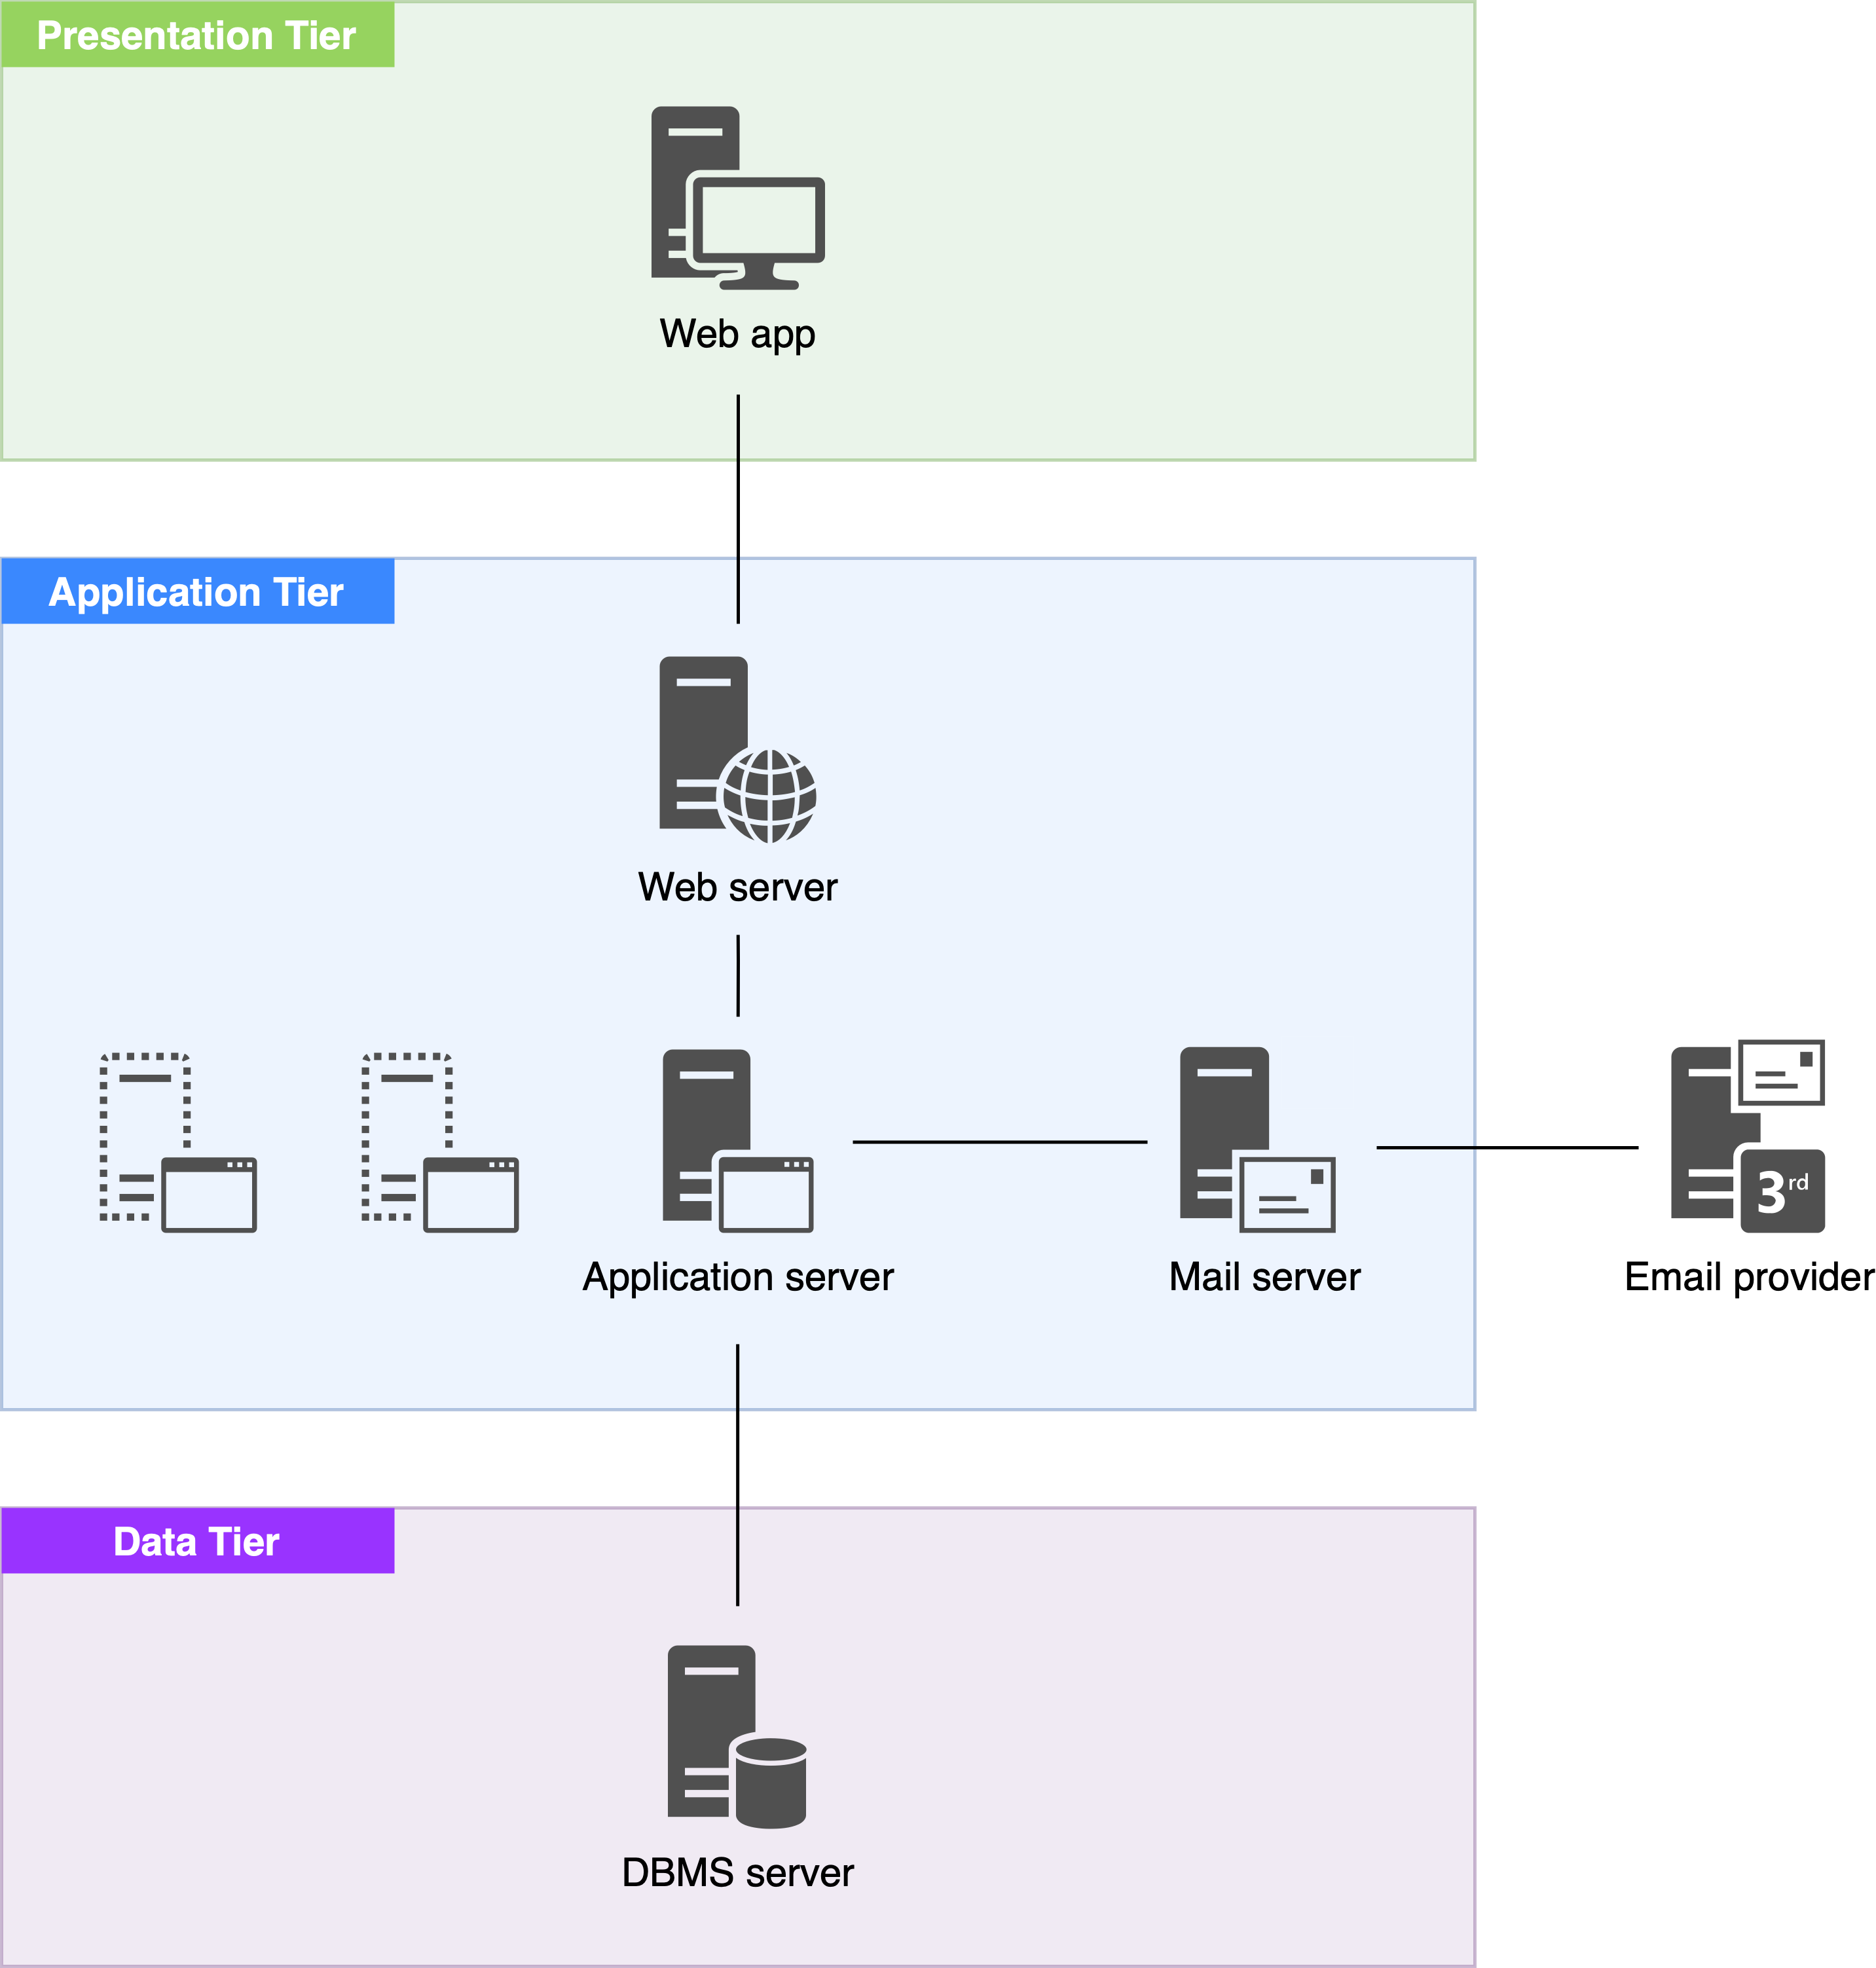
\includegraphics[width=14cm]{images/architecture.png}
    \caption{Architecture}
\end{figure}

\section{Component View}
This section illustrates the logical organization of Students\&Companies by breaking down the system into its major software modules and mapping their relationships.
Using a series of increasingly detailed diagrams, the component view first presents a high-level view showing the system elements and their interactions.
It then dives into individual components, examining their low-level structures, responsibilities and interfaces, with particular attention to how they collaborate to implement the platform's functionality.

\subsection{High-Level View}
The high-level diagram below shows the components of Students\&Companies and their interactions.
The application server exposes six interfaces to the web app, each corresponding to a domain of functionality that will be further discussed in the next section.

\begin{figure}[h]
    \centering
    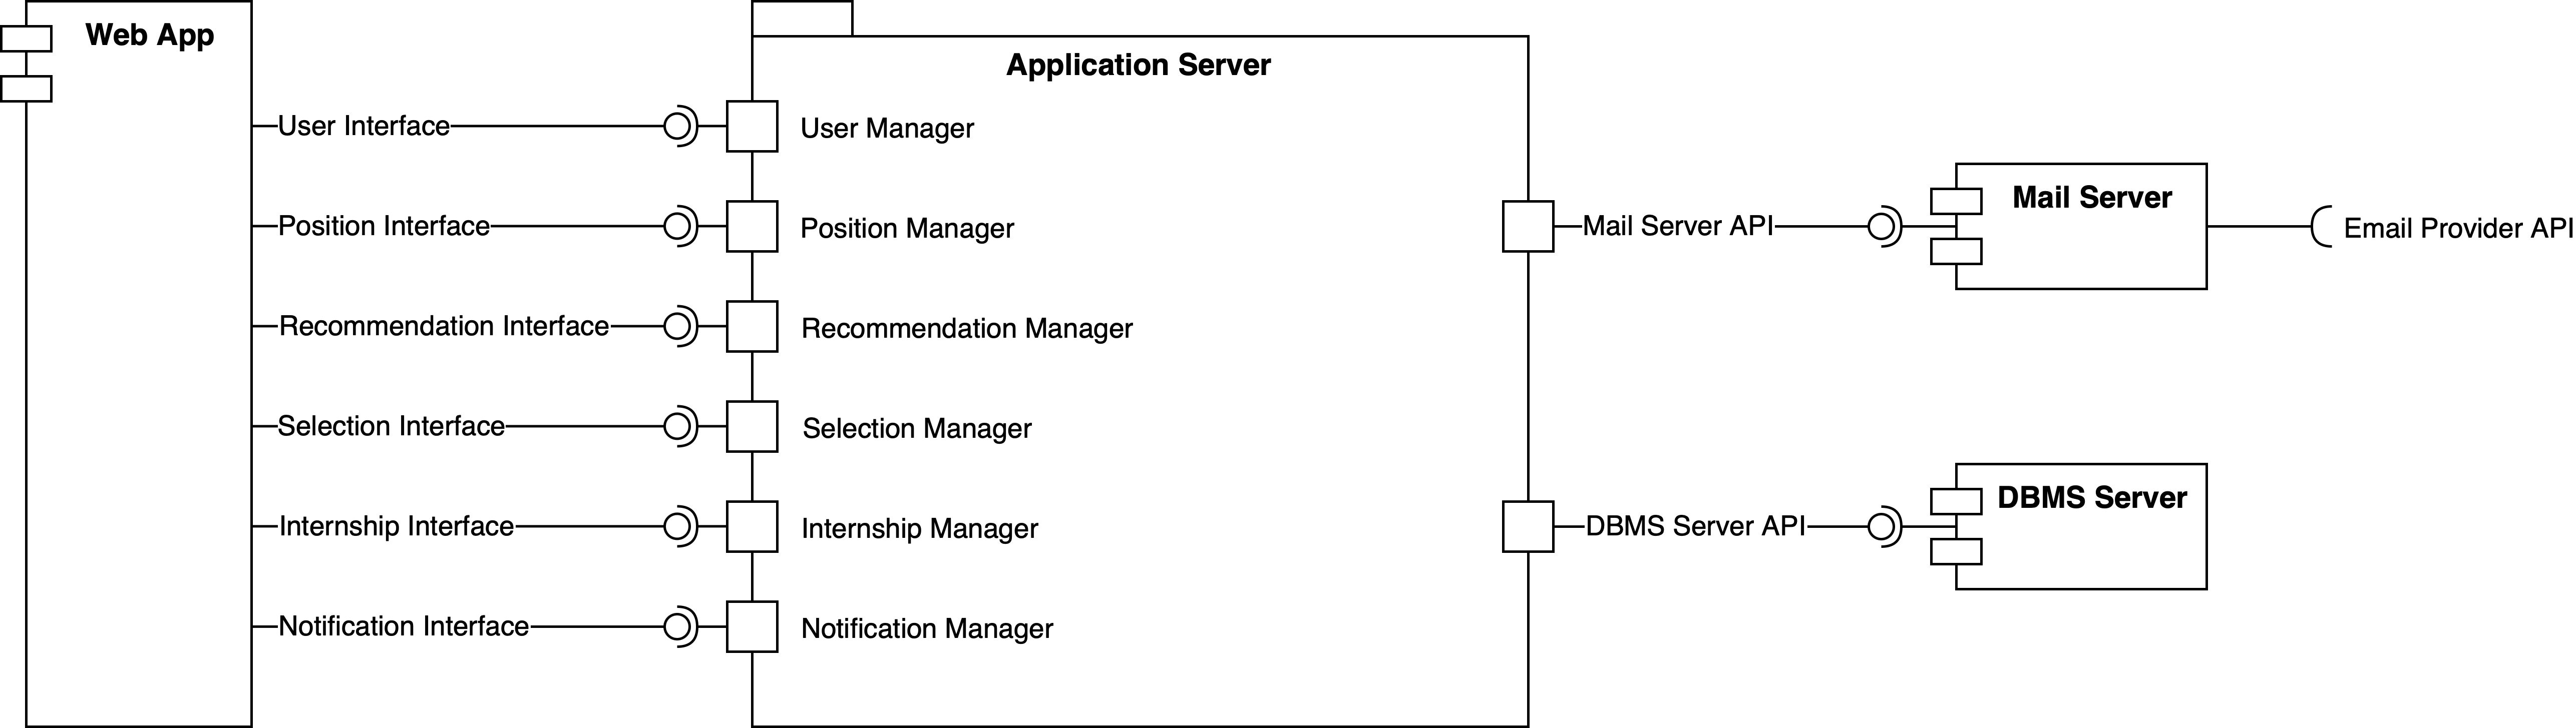
\includegraphics[width=16cm]{images/component-view/high-level.png}
    \caption{High-level component view}
\end{figure}

\subsection{Low-Level View}
The low-level view below builds upon the high-level diagram above by providing a detailed representation of the internal architecture of the application server.
The codebase is structured according to the model-view-controller pattern.
In this architecture, the model acts as the core data structure of the system, representing and managing the content of the database.
In turn, managers act as controllers, bridging the model and the external interfaces, which serve as the entry points for users, ensuring a clean separation of concerns that makes the system modular, scalable and maintainable.

\begin{figure}[ht]
    \centering
    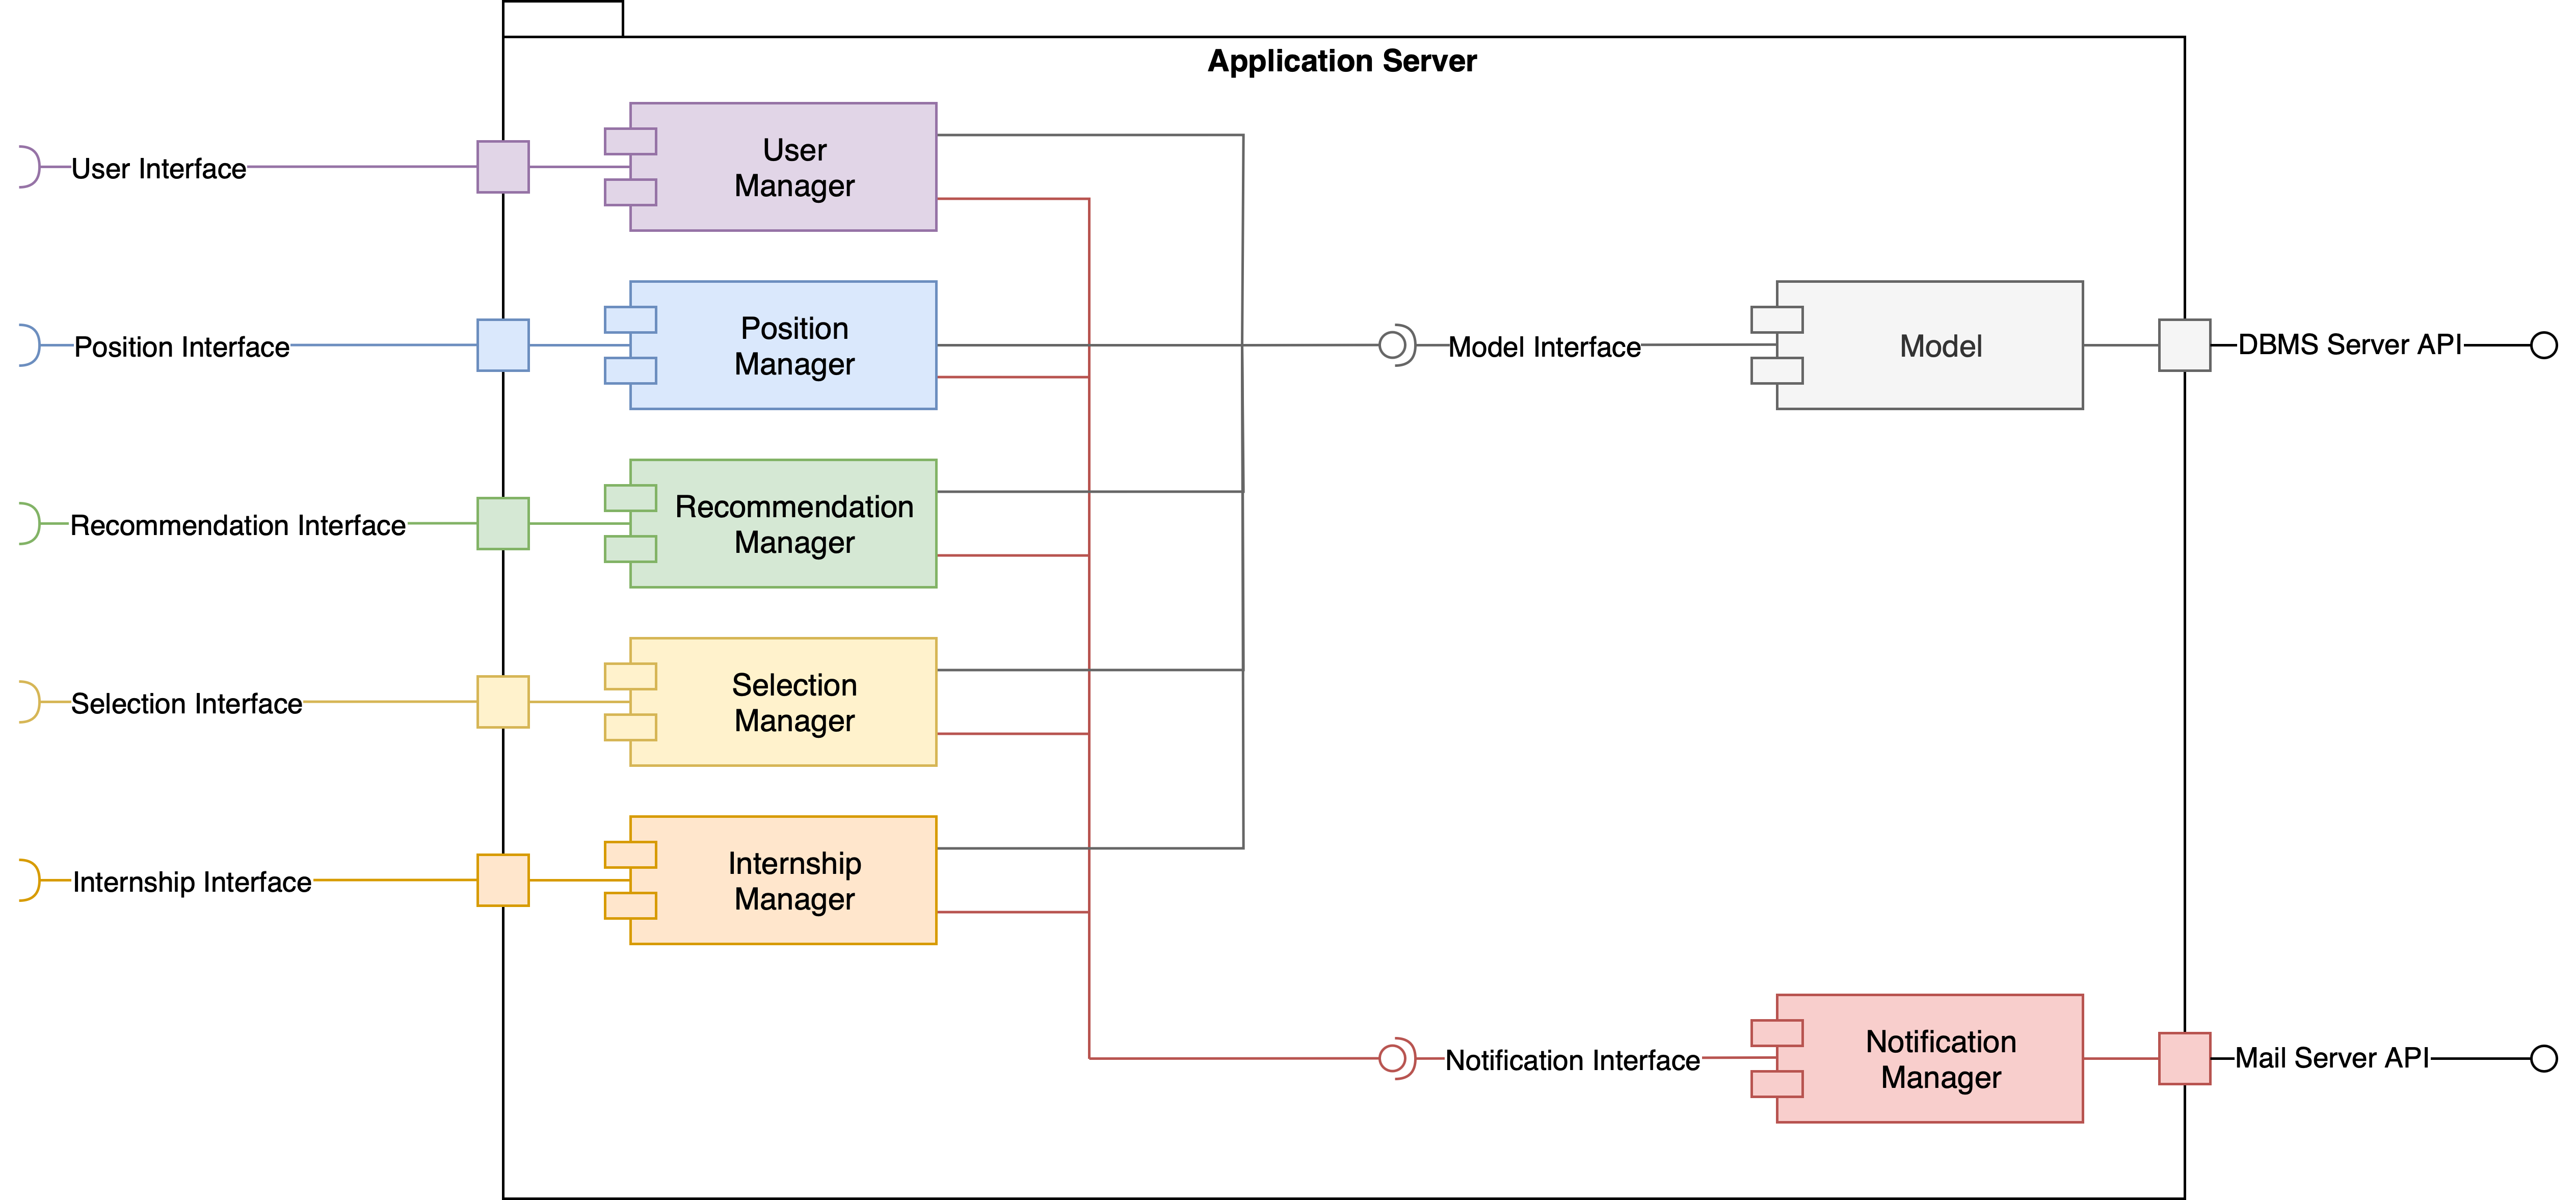
\includegraphics[width=16cm]{images/component-view/low-level.png}
    \caption{Low-level component view}
\end{figure}

Each manager is organized into multiple submanagers, which encapsulate specific functionalities within its domain.
These submanagers allow the managers to remain focused on their broader responsibilities while delegating finer tasks.
The following subsections delve into each manager, describing its role and breaking down its submanagers.

\subsubsection{User Manager}
The user interface serves as the bridge between users and the user manager, channeling requests related to account creation, authentication and management.

\begin{figure}[ht]
    \centering
    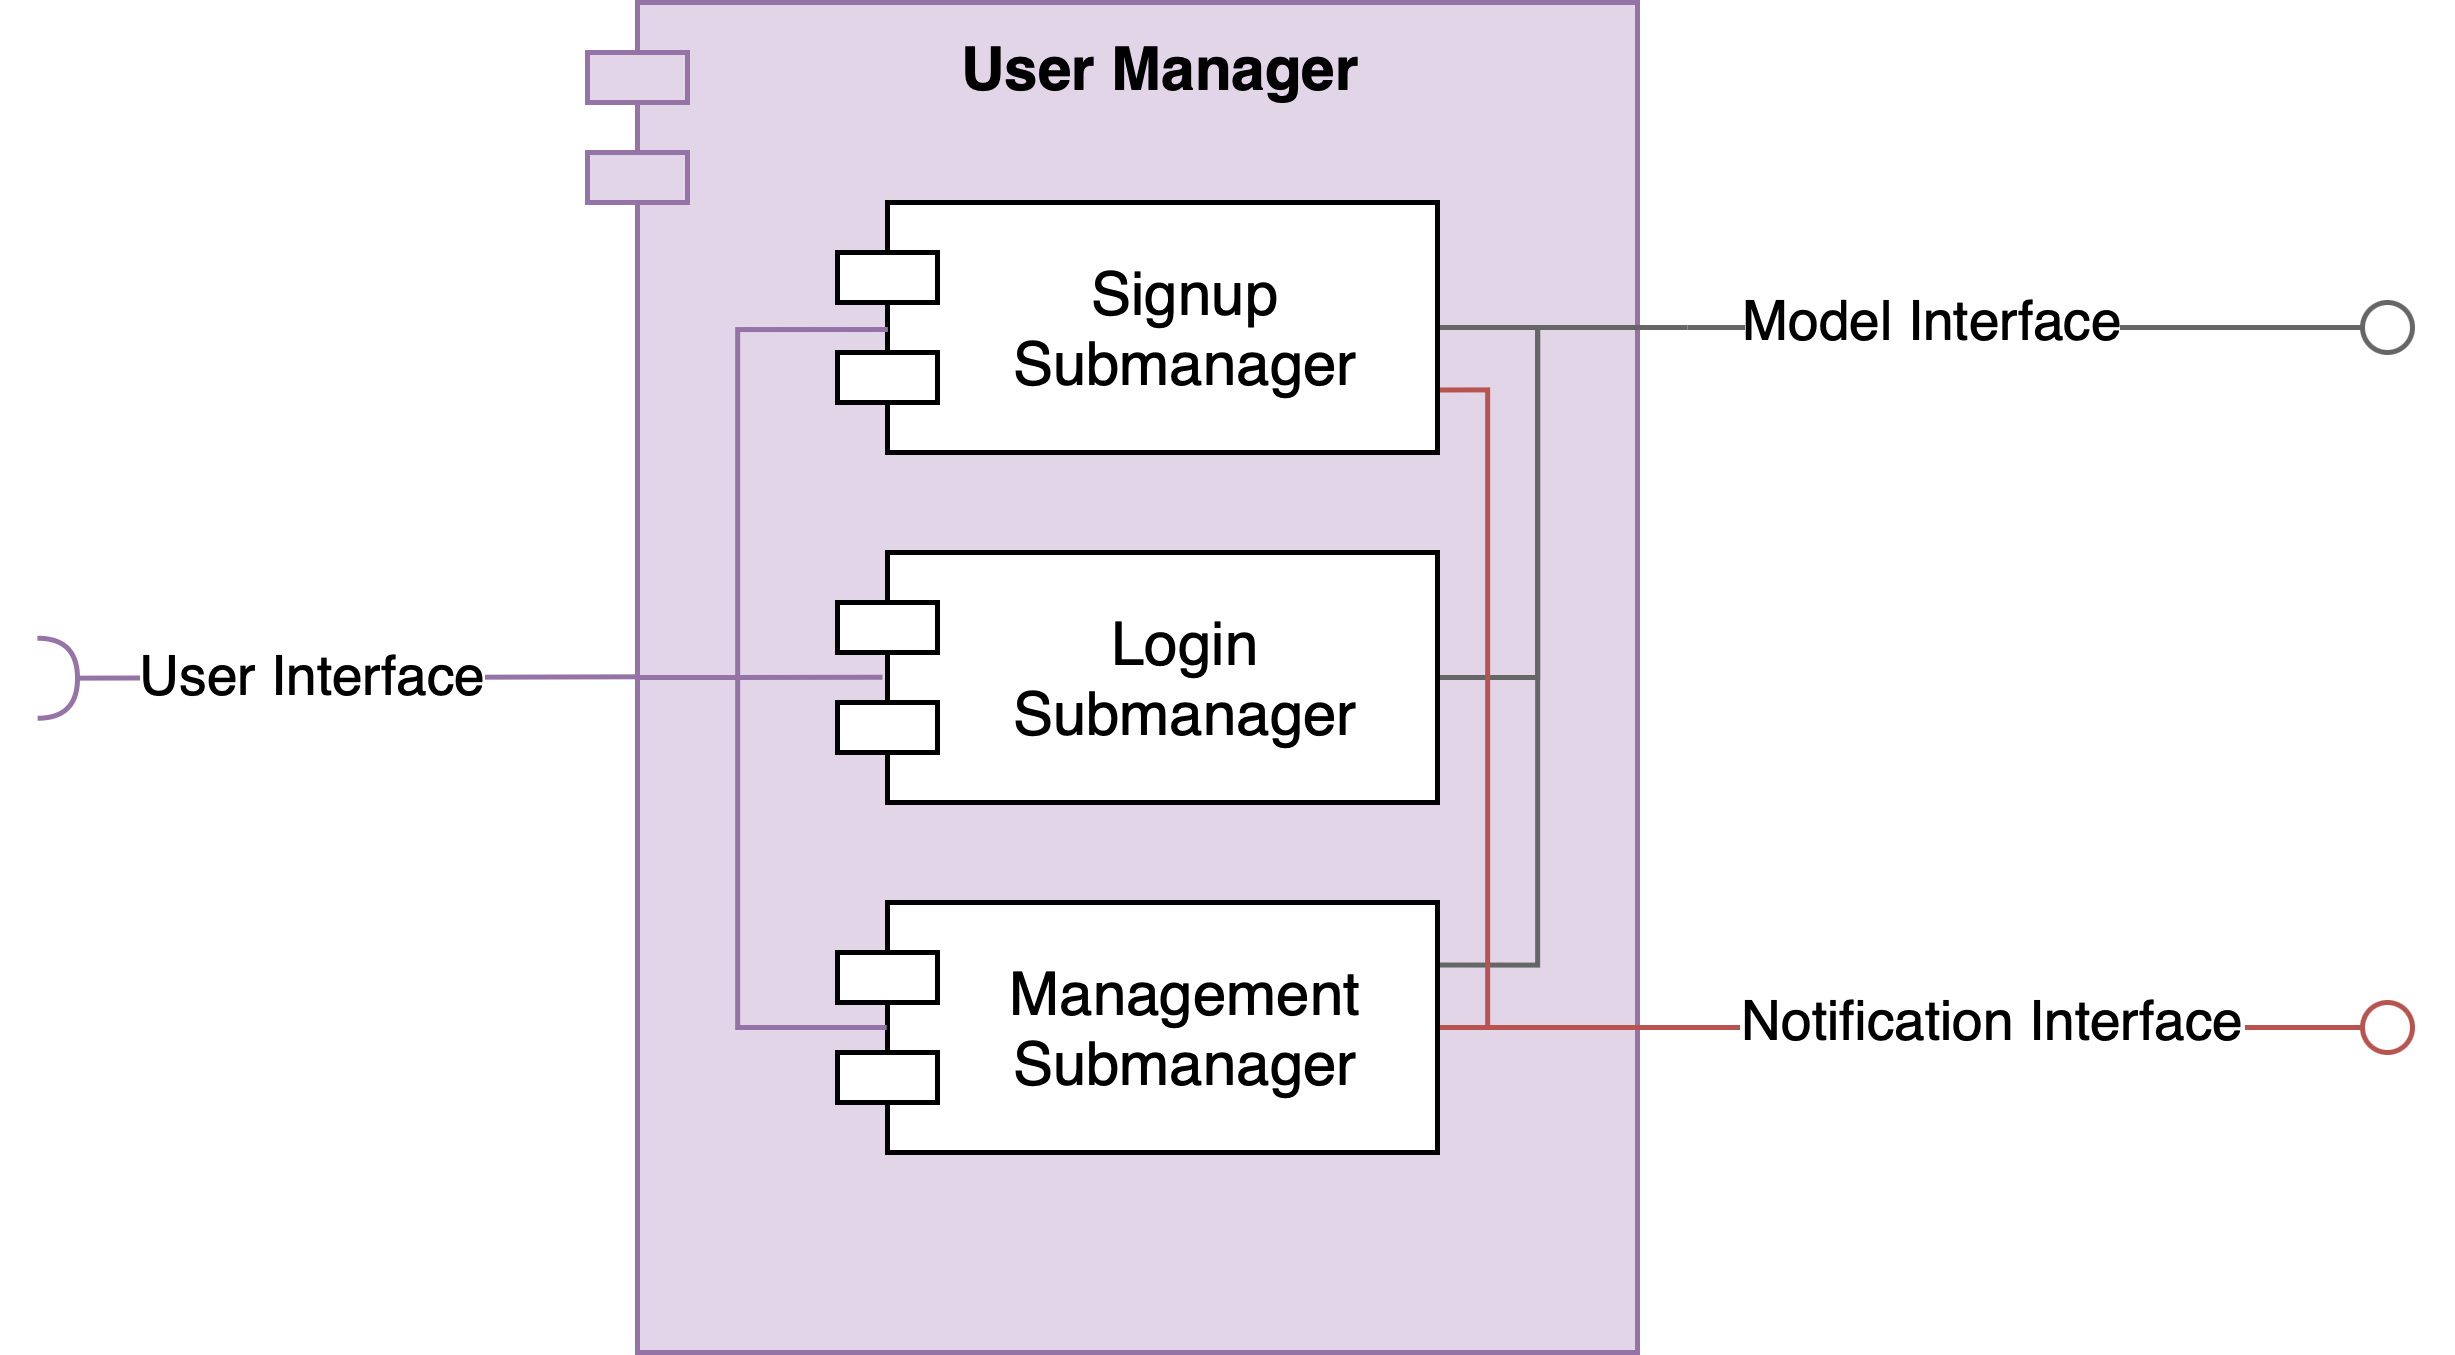
\includegraphics[width=11cm]{images/managers/user.png}
    \caption{User manager}
\end{figure}

The user signup submanager handles user onboarding by validating fields and enforcing rules like password length.
It securely integrates new users into the system while delegating confirmation emails to the notification manager.

The user login submanager supports user logins, validating credentials and issuing tokens for secure session management.
It also ensures that expired tokens are revoked.

The user management submanager supports users in updating their profiles, including editing preferences and uploading CVs, validating and storing changes.
Additionally, it provides an option for account deletion.

\subsubsection{Position Manager}
The position interface acts as the portal for managing internship postings, funneling requests from both companies and students to the position manager.
This manager ensures that opportunities are validated, maintained and accessible to all relevant users.

\begin{figure}[h]
    \centering
    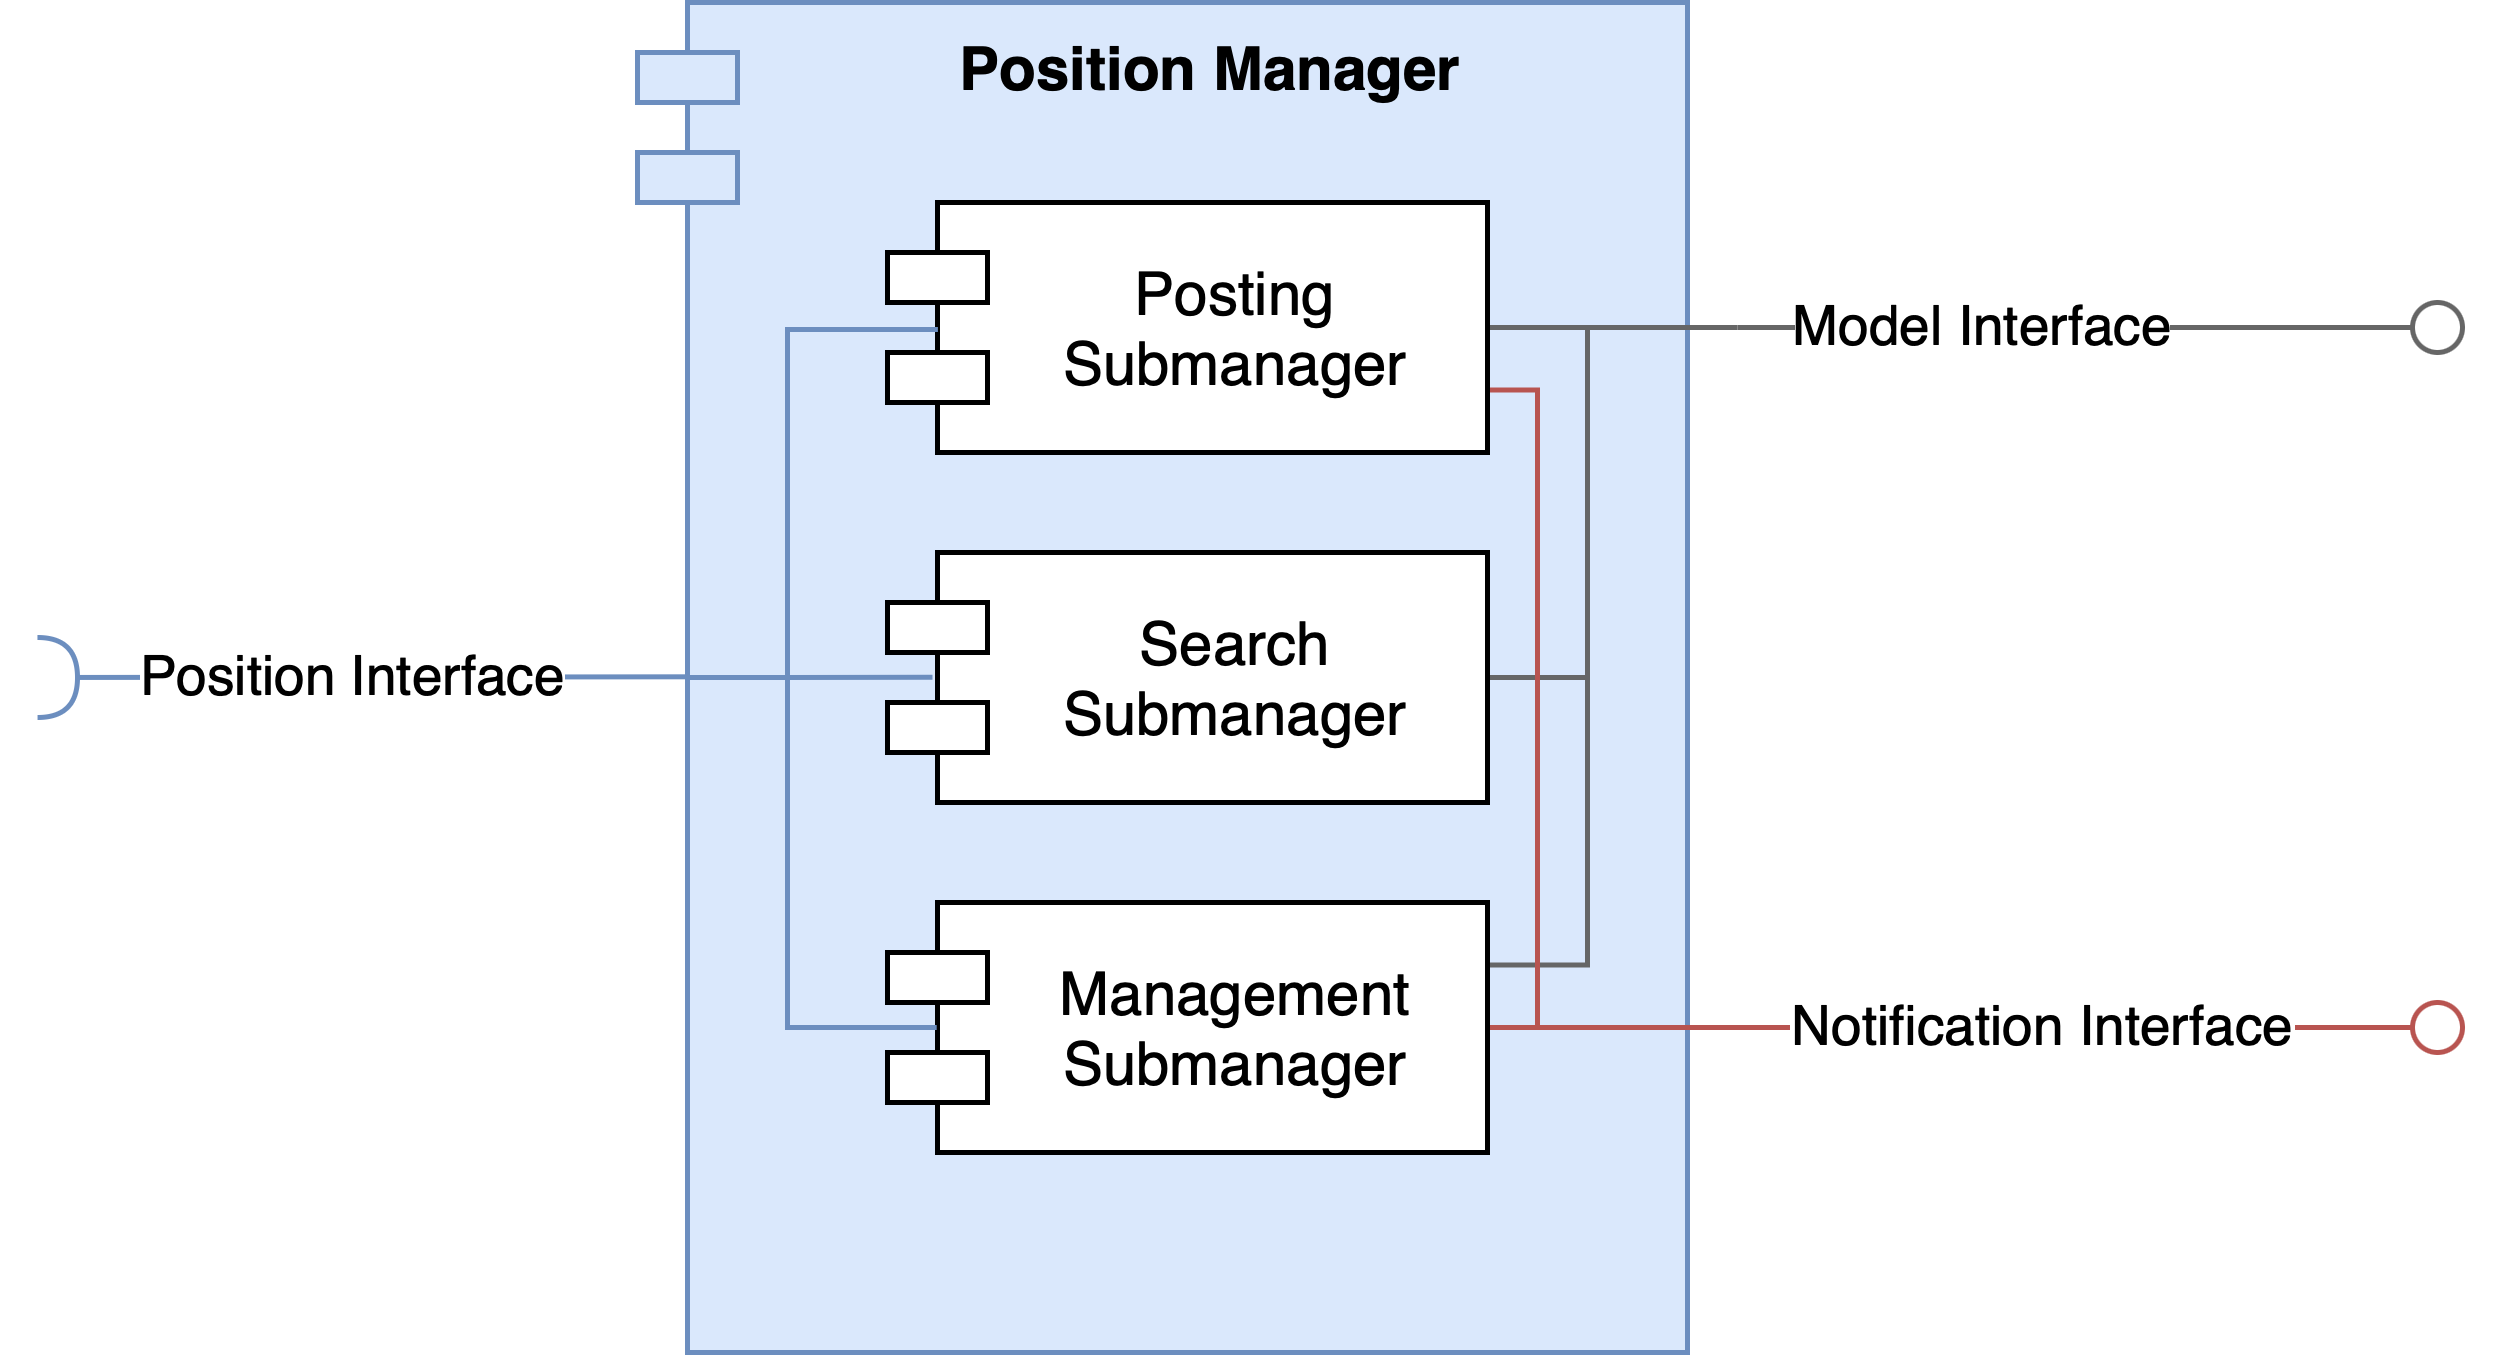
\includegraphics[width=11cm]{images/managers/position.png}
    \caption{Position manager}
\end{figure}

The position posting submanager allows companies to post new positions, validating details such as required skills and terms.

The position search submanager empowers students to search for opportunities through keywords.
It ranks and prioritizes results, highlighting the most relevant options.

The position management submanager supports companies in modifying existing position postings, ensuring all changes are logged, including updates in their status.

\subsubsection{Recommendation Manager}
The recommendation interface fuels the platform’s personalized experience by connecting users with tailored matches.
The recommendation manager transforms system data into actionable suggestions, enhancing engagement.

\begin{figure}[ht]
    \centering
    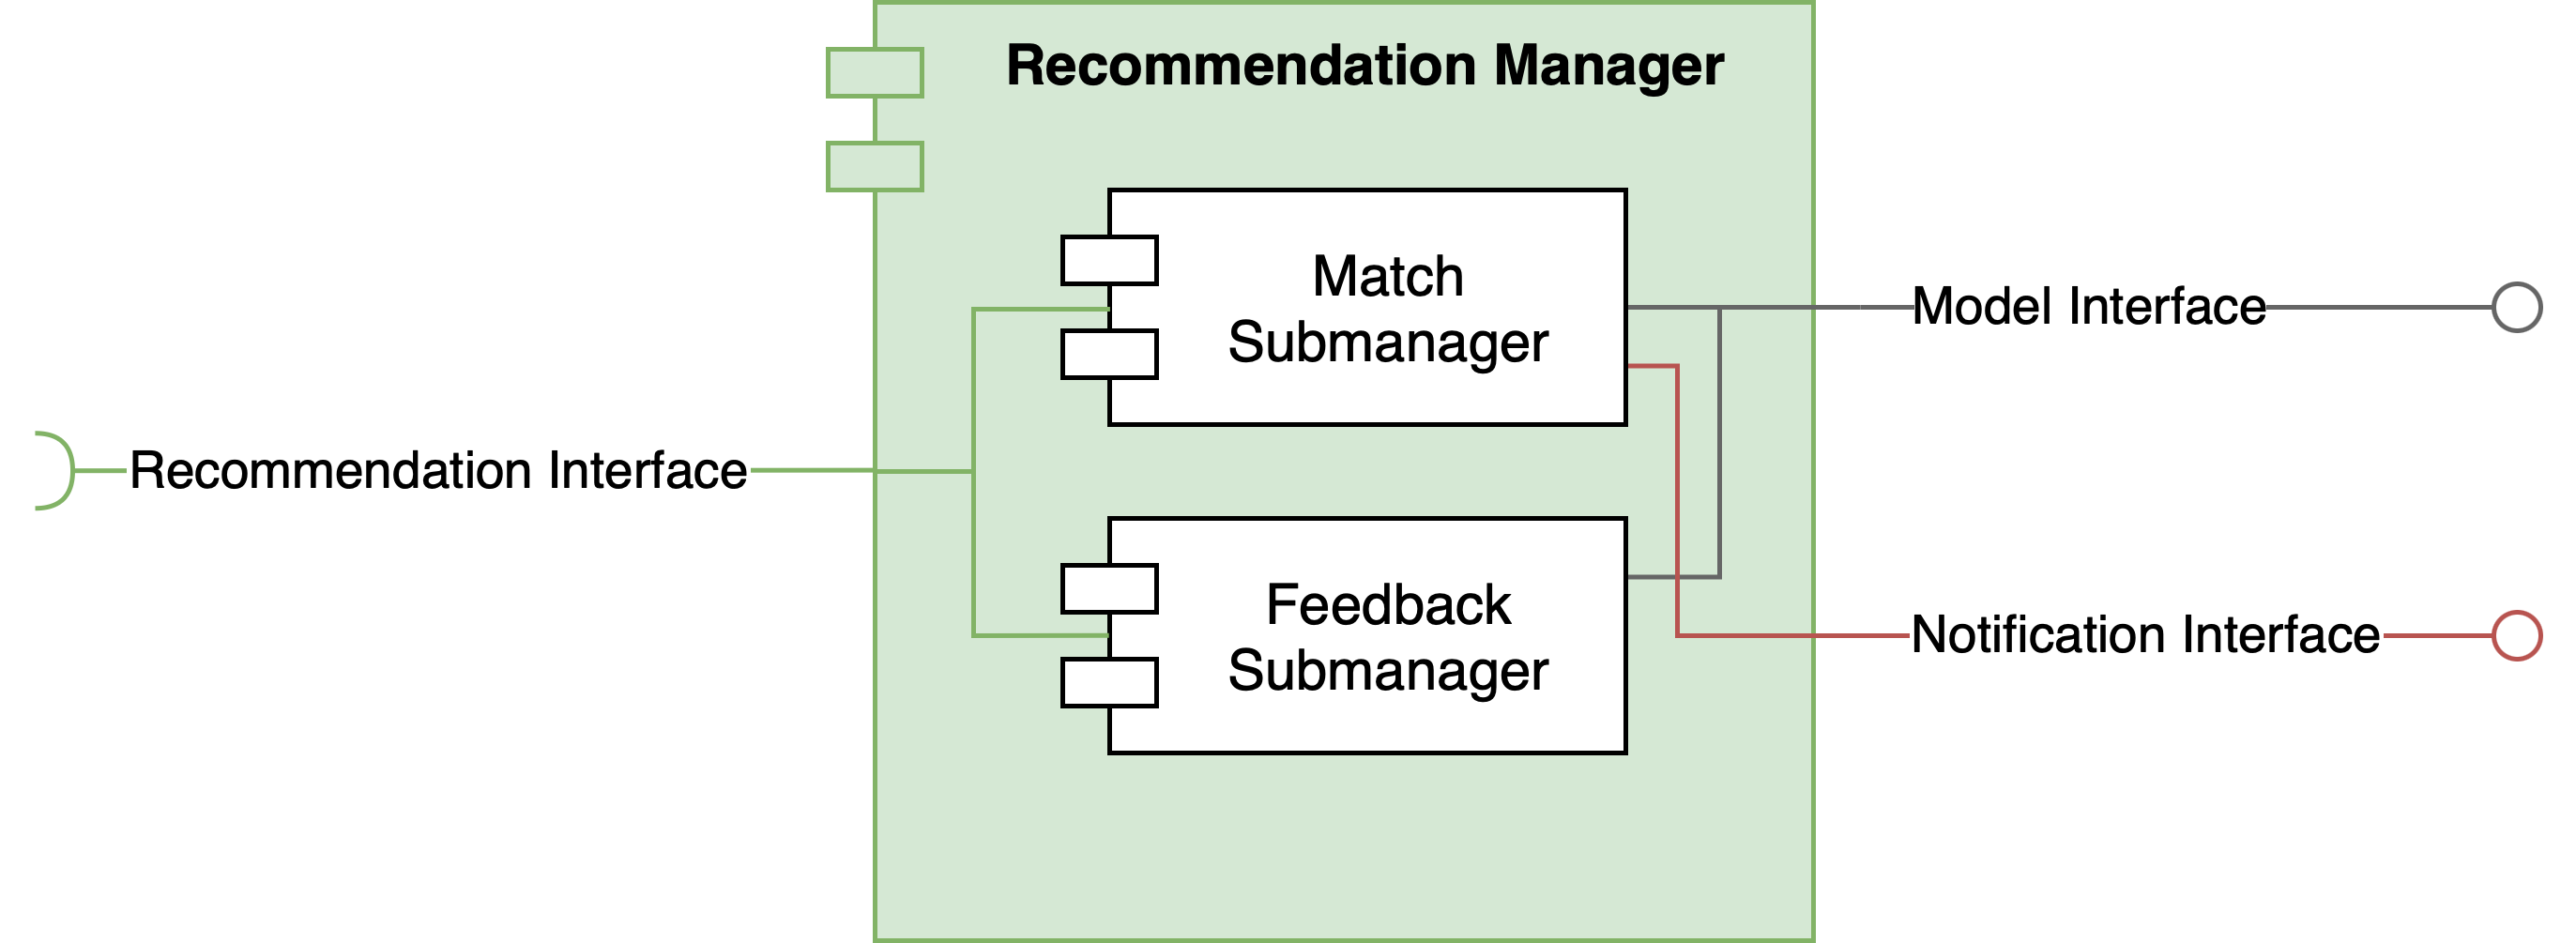
\includegraphics[width=12cm]{images/managers/recommendation.png}
    \caption{Recommendation manager}
\end{figure}

The recommendation match submanager applies statistical analysis to generate recommendations by comparing user profiles and position descriptions.
It also ensures users are informed about new recommendations by working with the notification manager.

The recommendation feedback submanager tracks feedback forms to refine future suggestions, improving relevance over time.

\subsubsection{Selection Manager}
The selection interface connects university students and companies through the selection process, channeling application and interview workflows to the selection manager.

\begin{figure}[h]
    \centering
    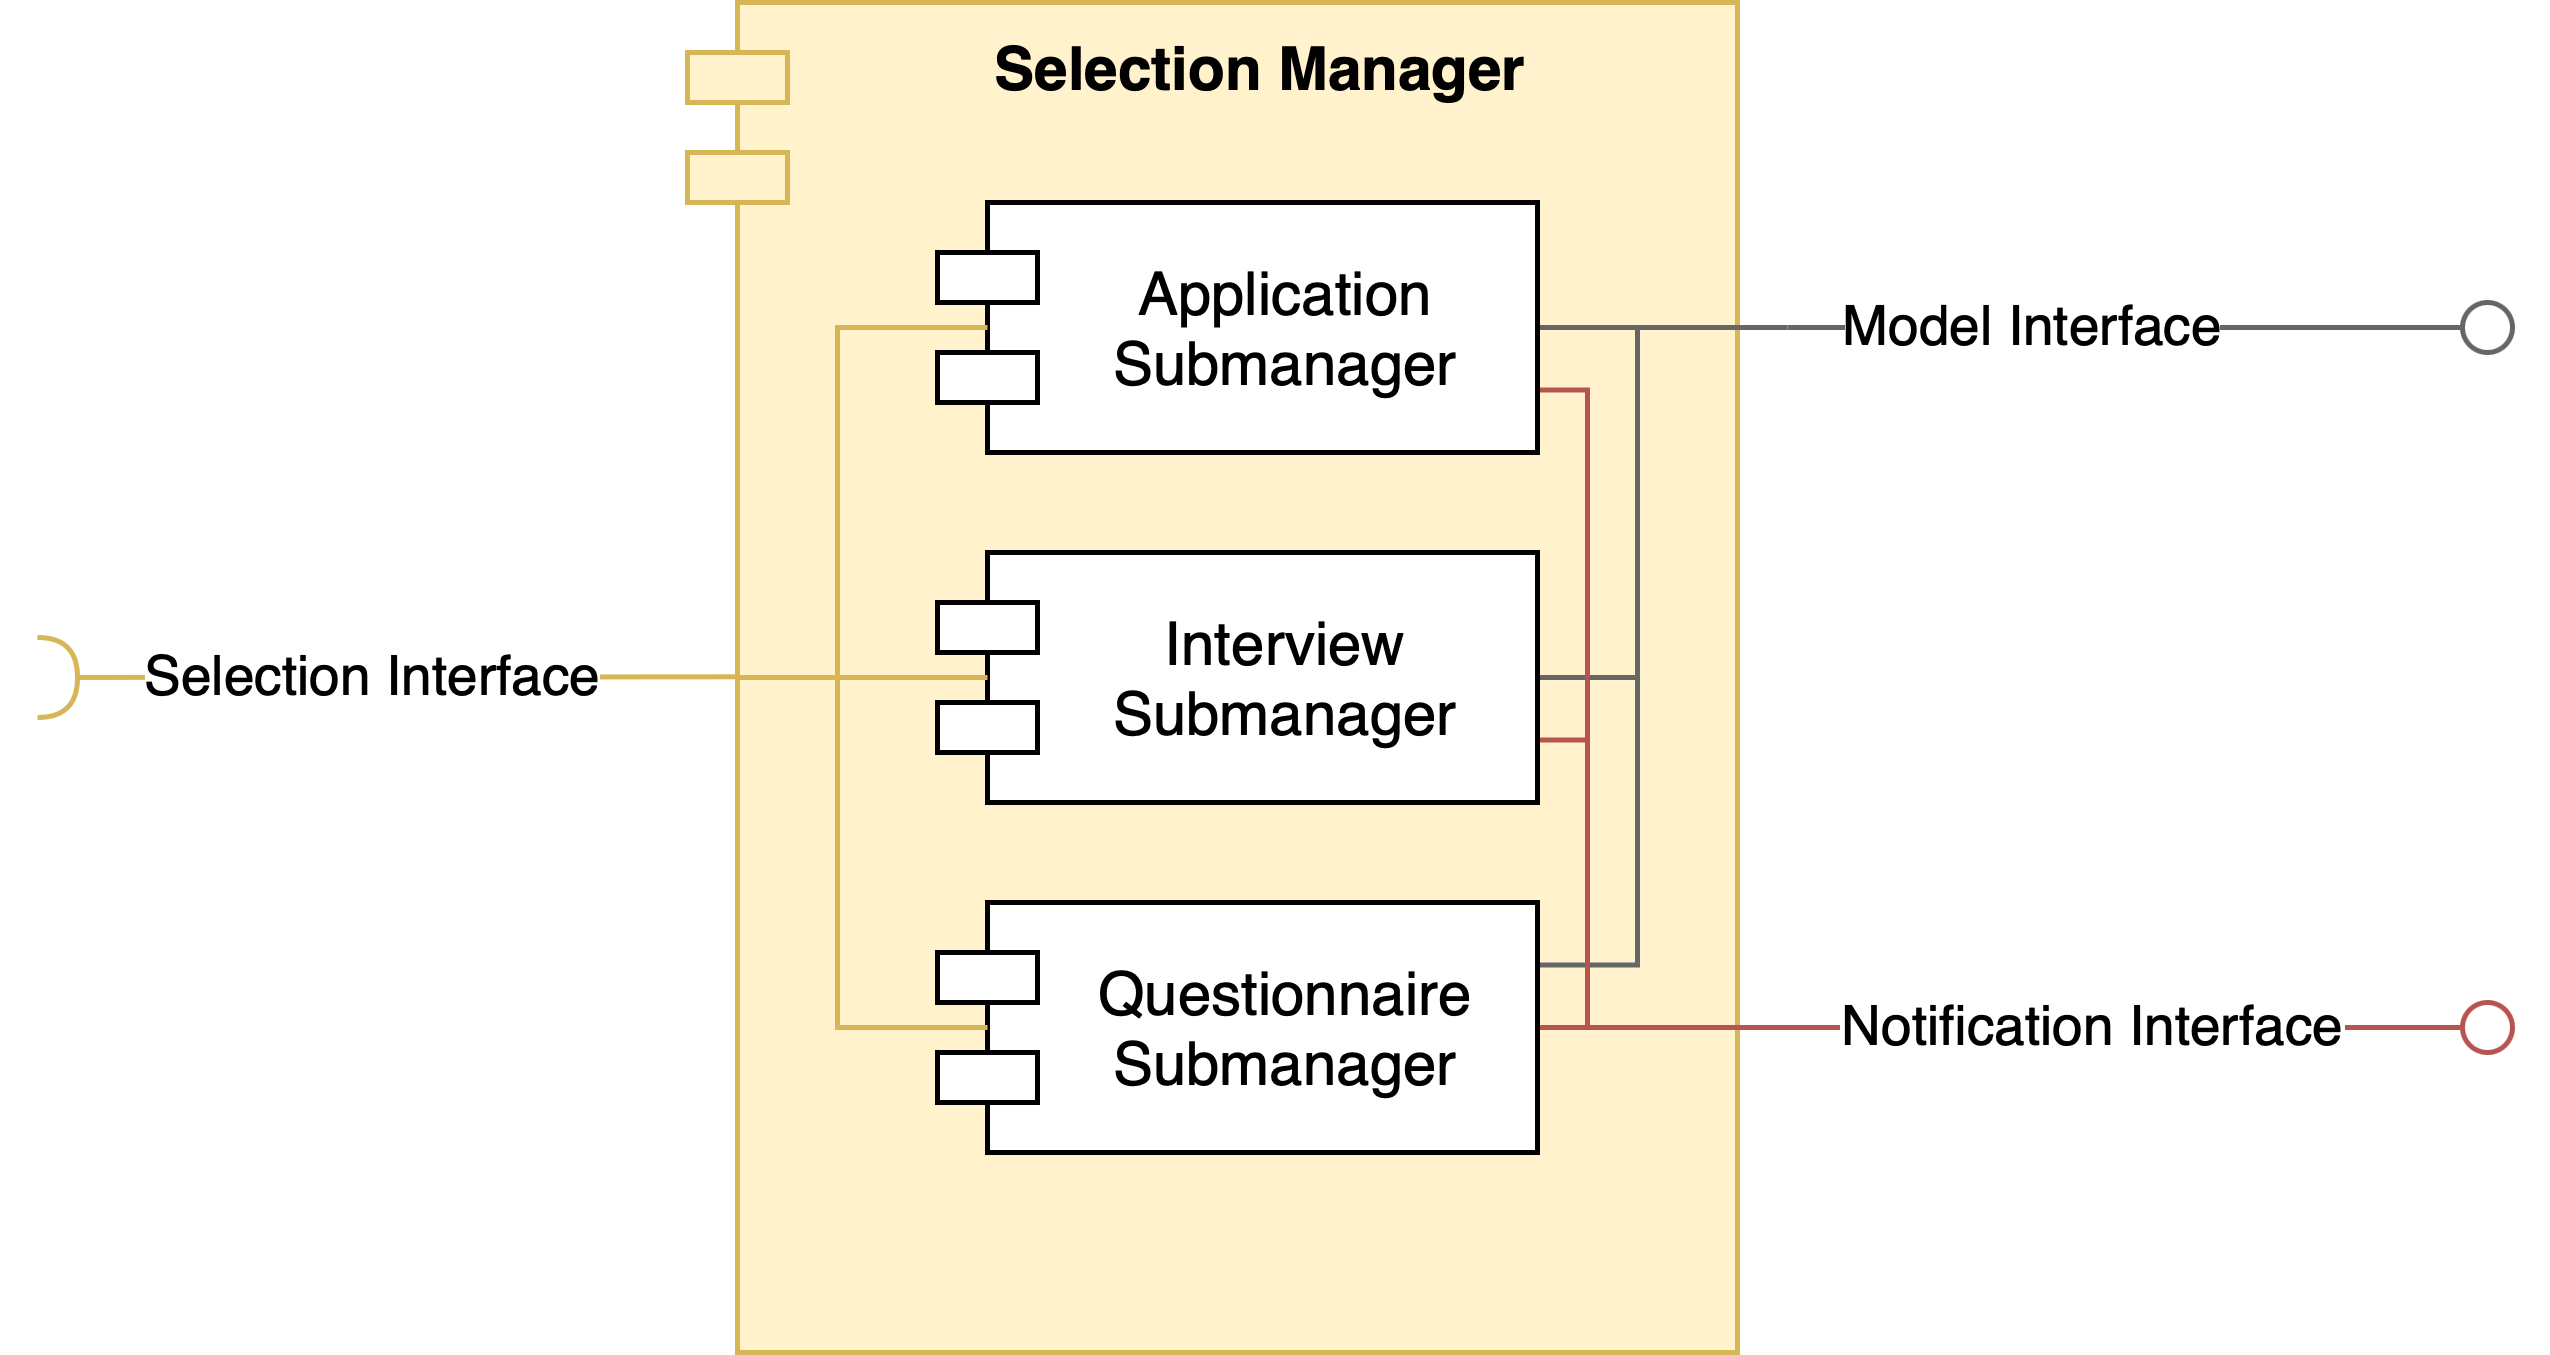
\includegraphics[width=11cm]{images/managers/selection.png}
    \caption{Selection manager}
\end{figure}

The selection application submanager oversees the lifecycle of applications, from initial submission to final outcome.
It makes sure that both students and companies are informed throughout the workflow by integrating with the notification manager.

The selection interview submanager coordinates interviews by validating availability and resolving conflicts, ensuring schedules are efficiently managed.

The selection questionnaire submanager supports companies in evaluating candidates by managing the distribution and storage of questionnaires.

\subsubsection{Internship Manager}
The internship interface facilitates collaboration among students, companies and universities, channeling related workflows to the internship manager.
This manager monitors ongoing internships, ensuring transparency.

\begin{figure}[h]
    \centering
    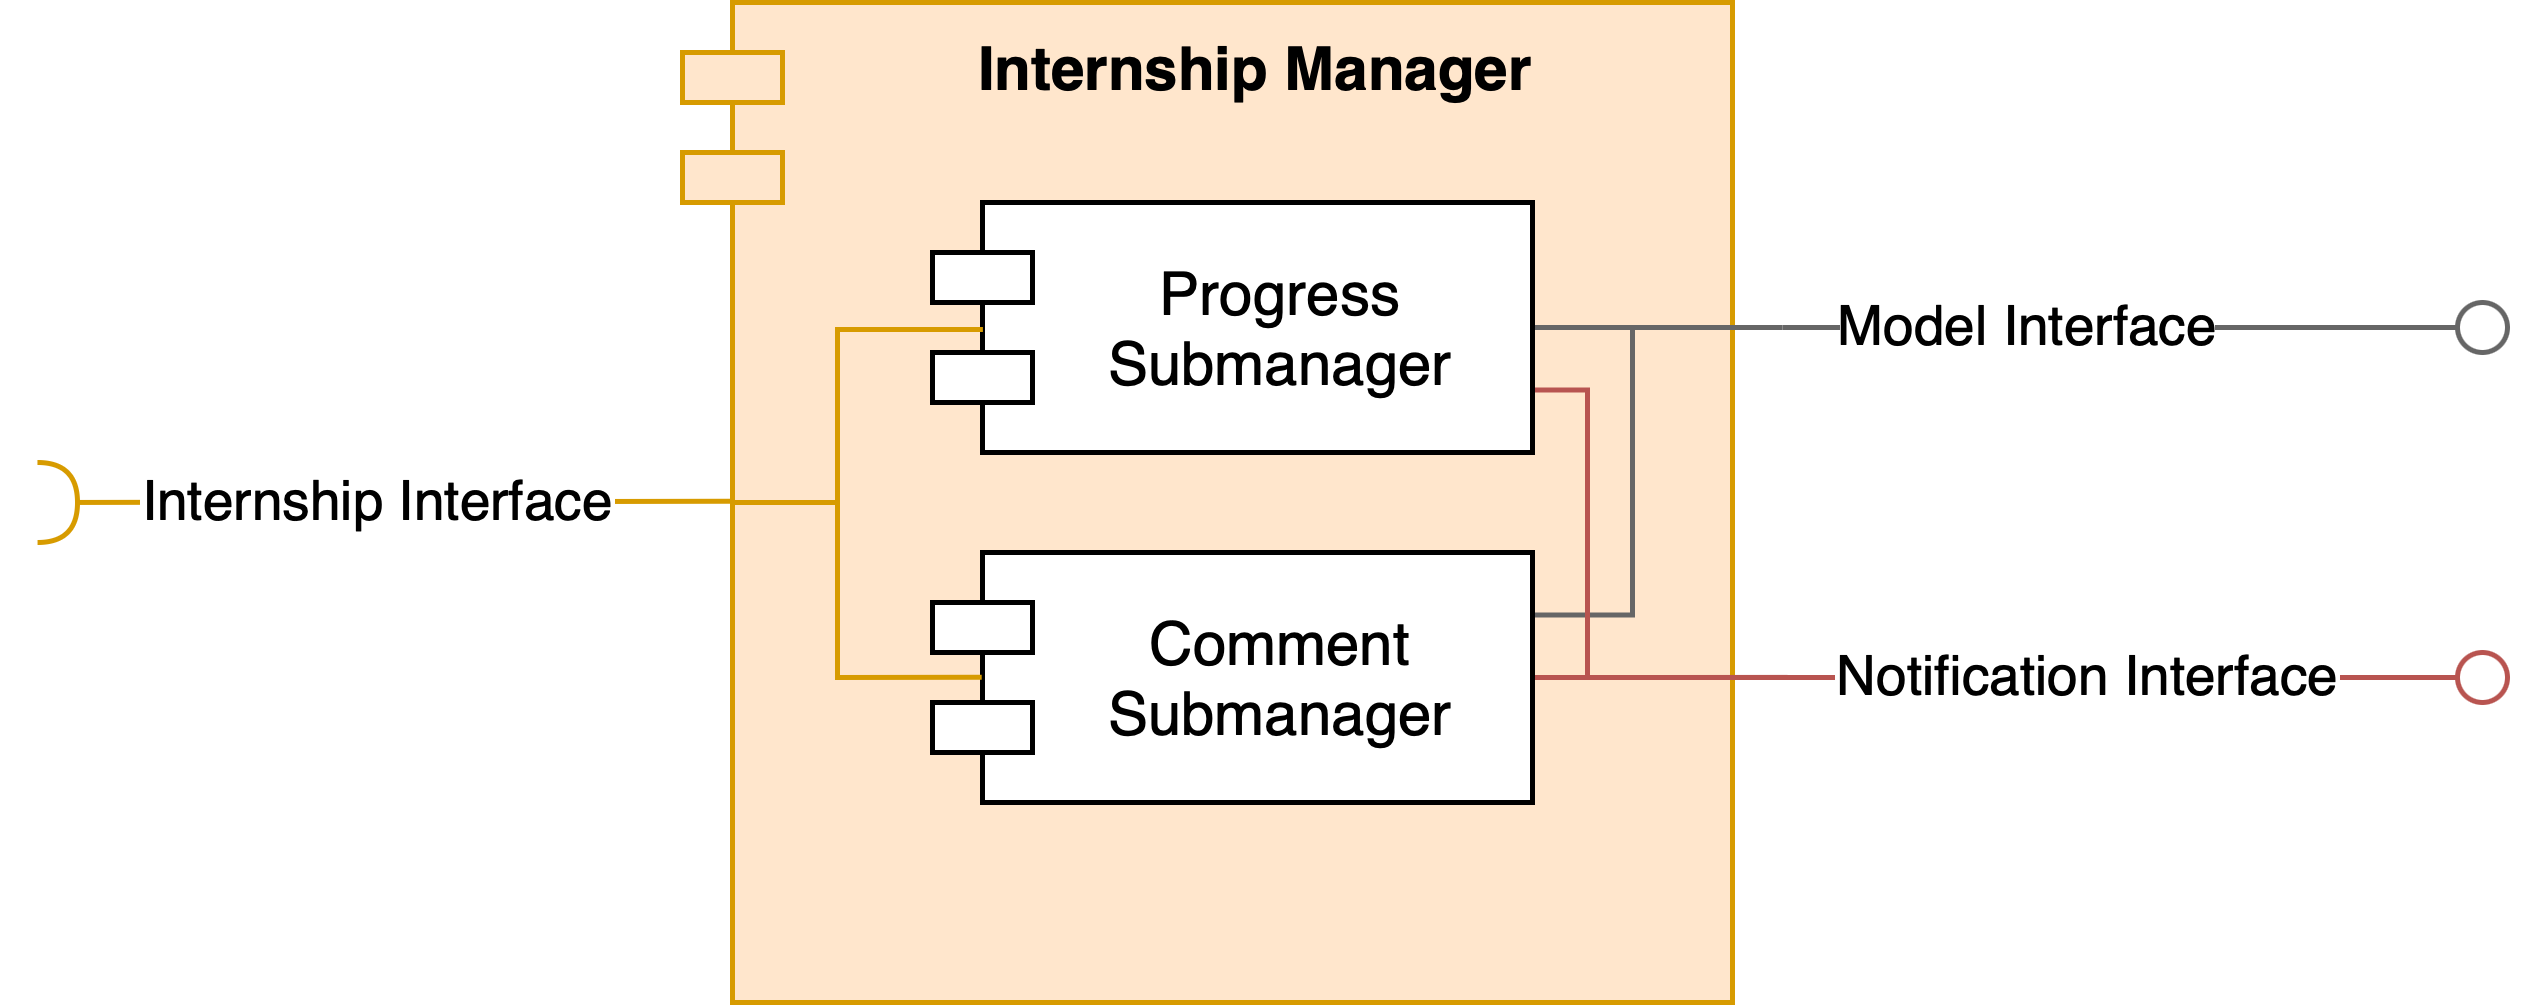
\includegraphics[width=11cm]{images/managers/internship.png}
    \caption{Internship manager}
\end{figure}

The internship progress submanager records status updates, providing all stakeholders with insights into internship progress.
Additionally, it collaborates with the notification manager to send update emails.

The internship comment submanager coordinates the posting of comments when progress is reported or a concern is raised.

\subsubsection{Notification Manager}
The notification interface connects other managers to the notification manager, which acts as the centralized hub for preparing and sending all emails.
By consolidating communication, it ensures consistency and reliability across the system.

\begin{figure}[h]
    \centering
    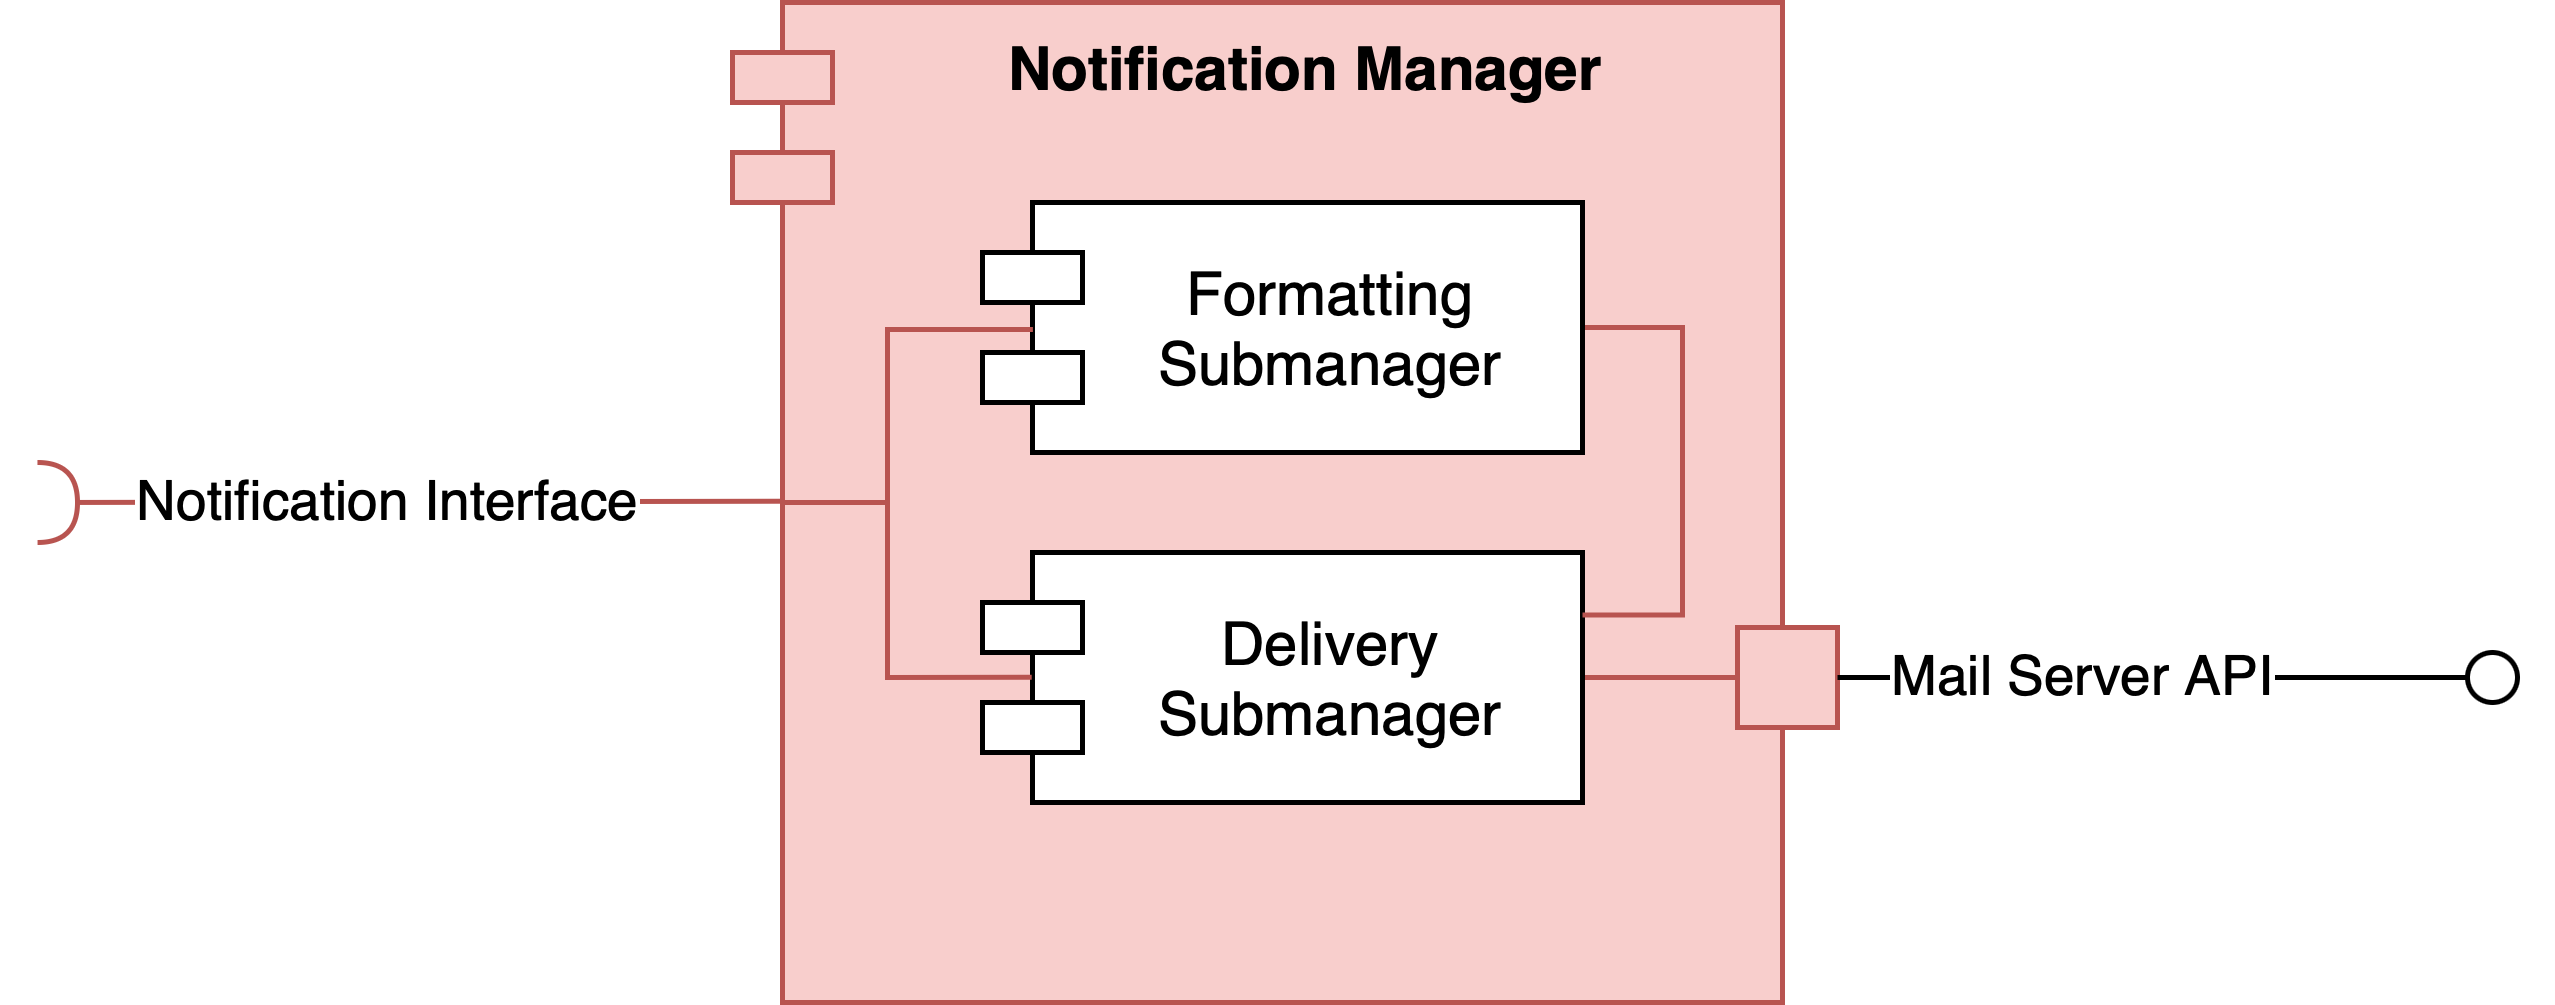
\includegraphics[width=11cm]{images/managers/notification.png}
    \caption{Notification manager}
\end{figure}

The notification formatting submanager prepares emails by structuring data provided by other managers, ensuring clarity for the recipient.

The notification delivery submanager communicates with the mail server API to send notifications, tracking delivery and retrying failed attempts to maintain reliability.

\section{Deployment View}
This section provides a detailed representation of how the software components are physically deployed on hardware nodes, together with their interactions.
It outlines the infrastructure, focusing on the communication protocols, security measures and data management strategies employed in the system.
The deployment view below is designed to align with the three-tier architecture defined in the overview.

\begin{figure}[ht]
    \centering
    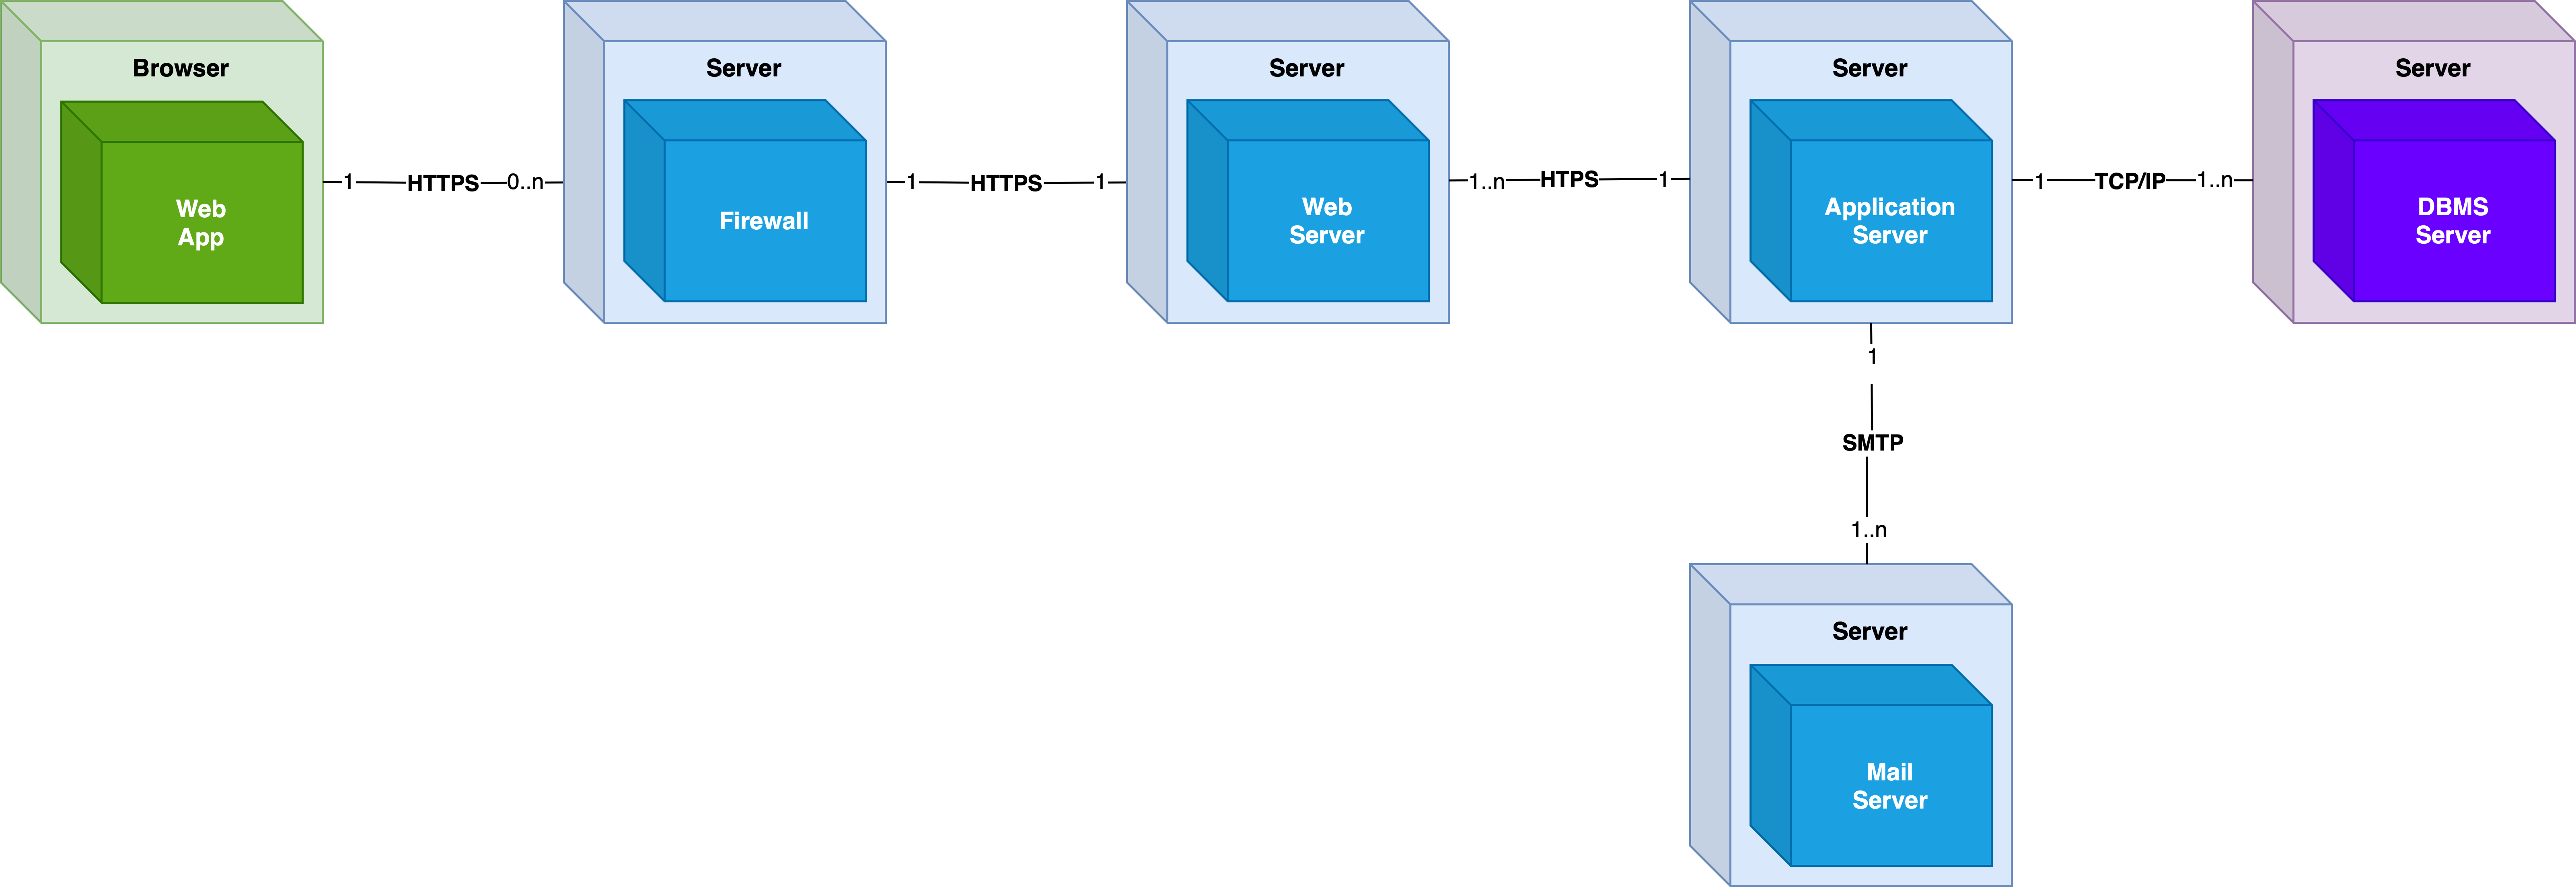
\includegraphics[width=16cm]{images/deployment-view.png}
    \caption{Deployment view}
\end{figure}

A firewall is deployed between the browser and the web server to protect the internal infrastructure.
It acts as the first line of defense by filtering incoming traffic and allowing only HTTPS requests on designated ports.
This ensures that exclusively legitimate traffic reaches the web server, mitigating risks of unauthorized access or malicious attacks.

The connection between the firewall and the web server, and subsequently between the web server and the application server, uses HTTPS.
This protocol encrypts all transmitted data, ensuring confidentiality and integrity for securing sensitive operations such as user authentication.
The application server then communicates with the DBMS server using the TCP/IP protocol, providing reliable and ordered data exchange.
This is suitable for database queries and responses, ensuring accurate transactions between the application and the database.
Lastly, the application server interacts with the mail server to send emails using SMTP.
This ensures efficient email delivery while separating email-related tasks from core ones.

A relational database management system like PostgreSQL is used for structured data storage, providing ACID compliance on a well-defined schema.
As they represent unstructured data, files such as uploaded CVs are stored locally on the DBMS server’s file system.
Rather than storing the binary data in the database itself, the file paths are saved as references in it instead.
This approach thus separates structured from unstructured data, optimizing database performance and simplifying file management.

\section{Runtime View}
The runtime view captures the dynamic behavior of the system by detailing how its components interact to perform specific operations.
Using sequence diagrams, this section illustrates the communication pathways and timing relationships among components, offering insights into the system's execution flow.
These runtime perspectives not only guide implementation but also serve as a reference for testing and troubleshooting.

\clearpage
\subsection{User}
\subsubsection{User Logs Out}
The user is logged in and on the home page.

\begin{figure}[h]
    \centering
    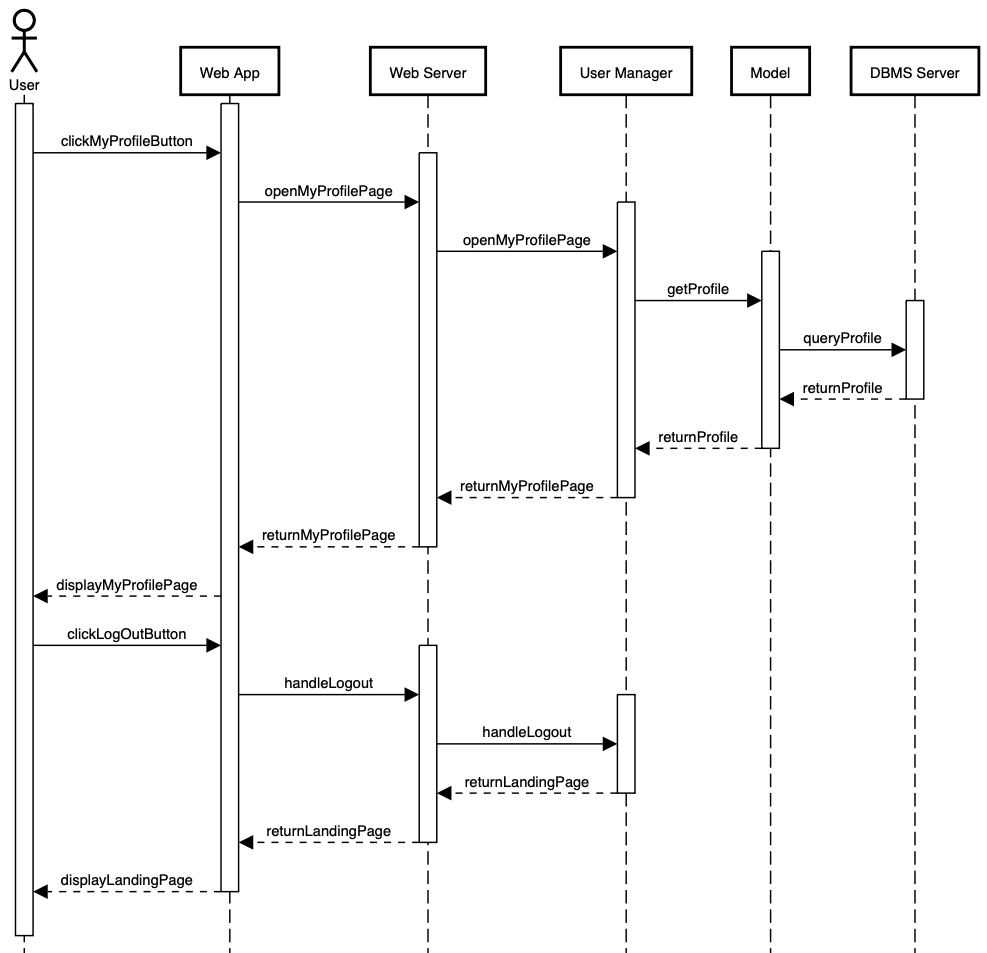
\includegraphics[width=16cm]{images/sequence-diagrams/user-logs-out.png}
    \caption{User logs out sequence diagram}
\end{figure}

\clearpage
\subsection{Student}
\subsubsection{Student Signs Up}
The student is not signed up.

\begin{figure}[h!]
    \centering
    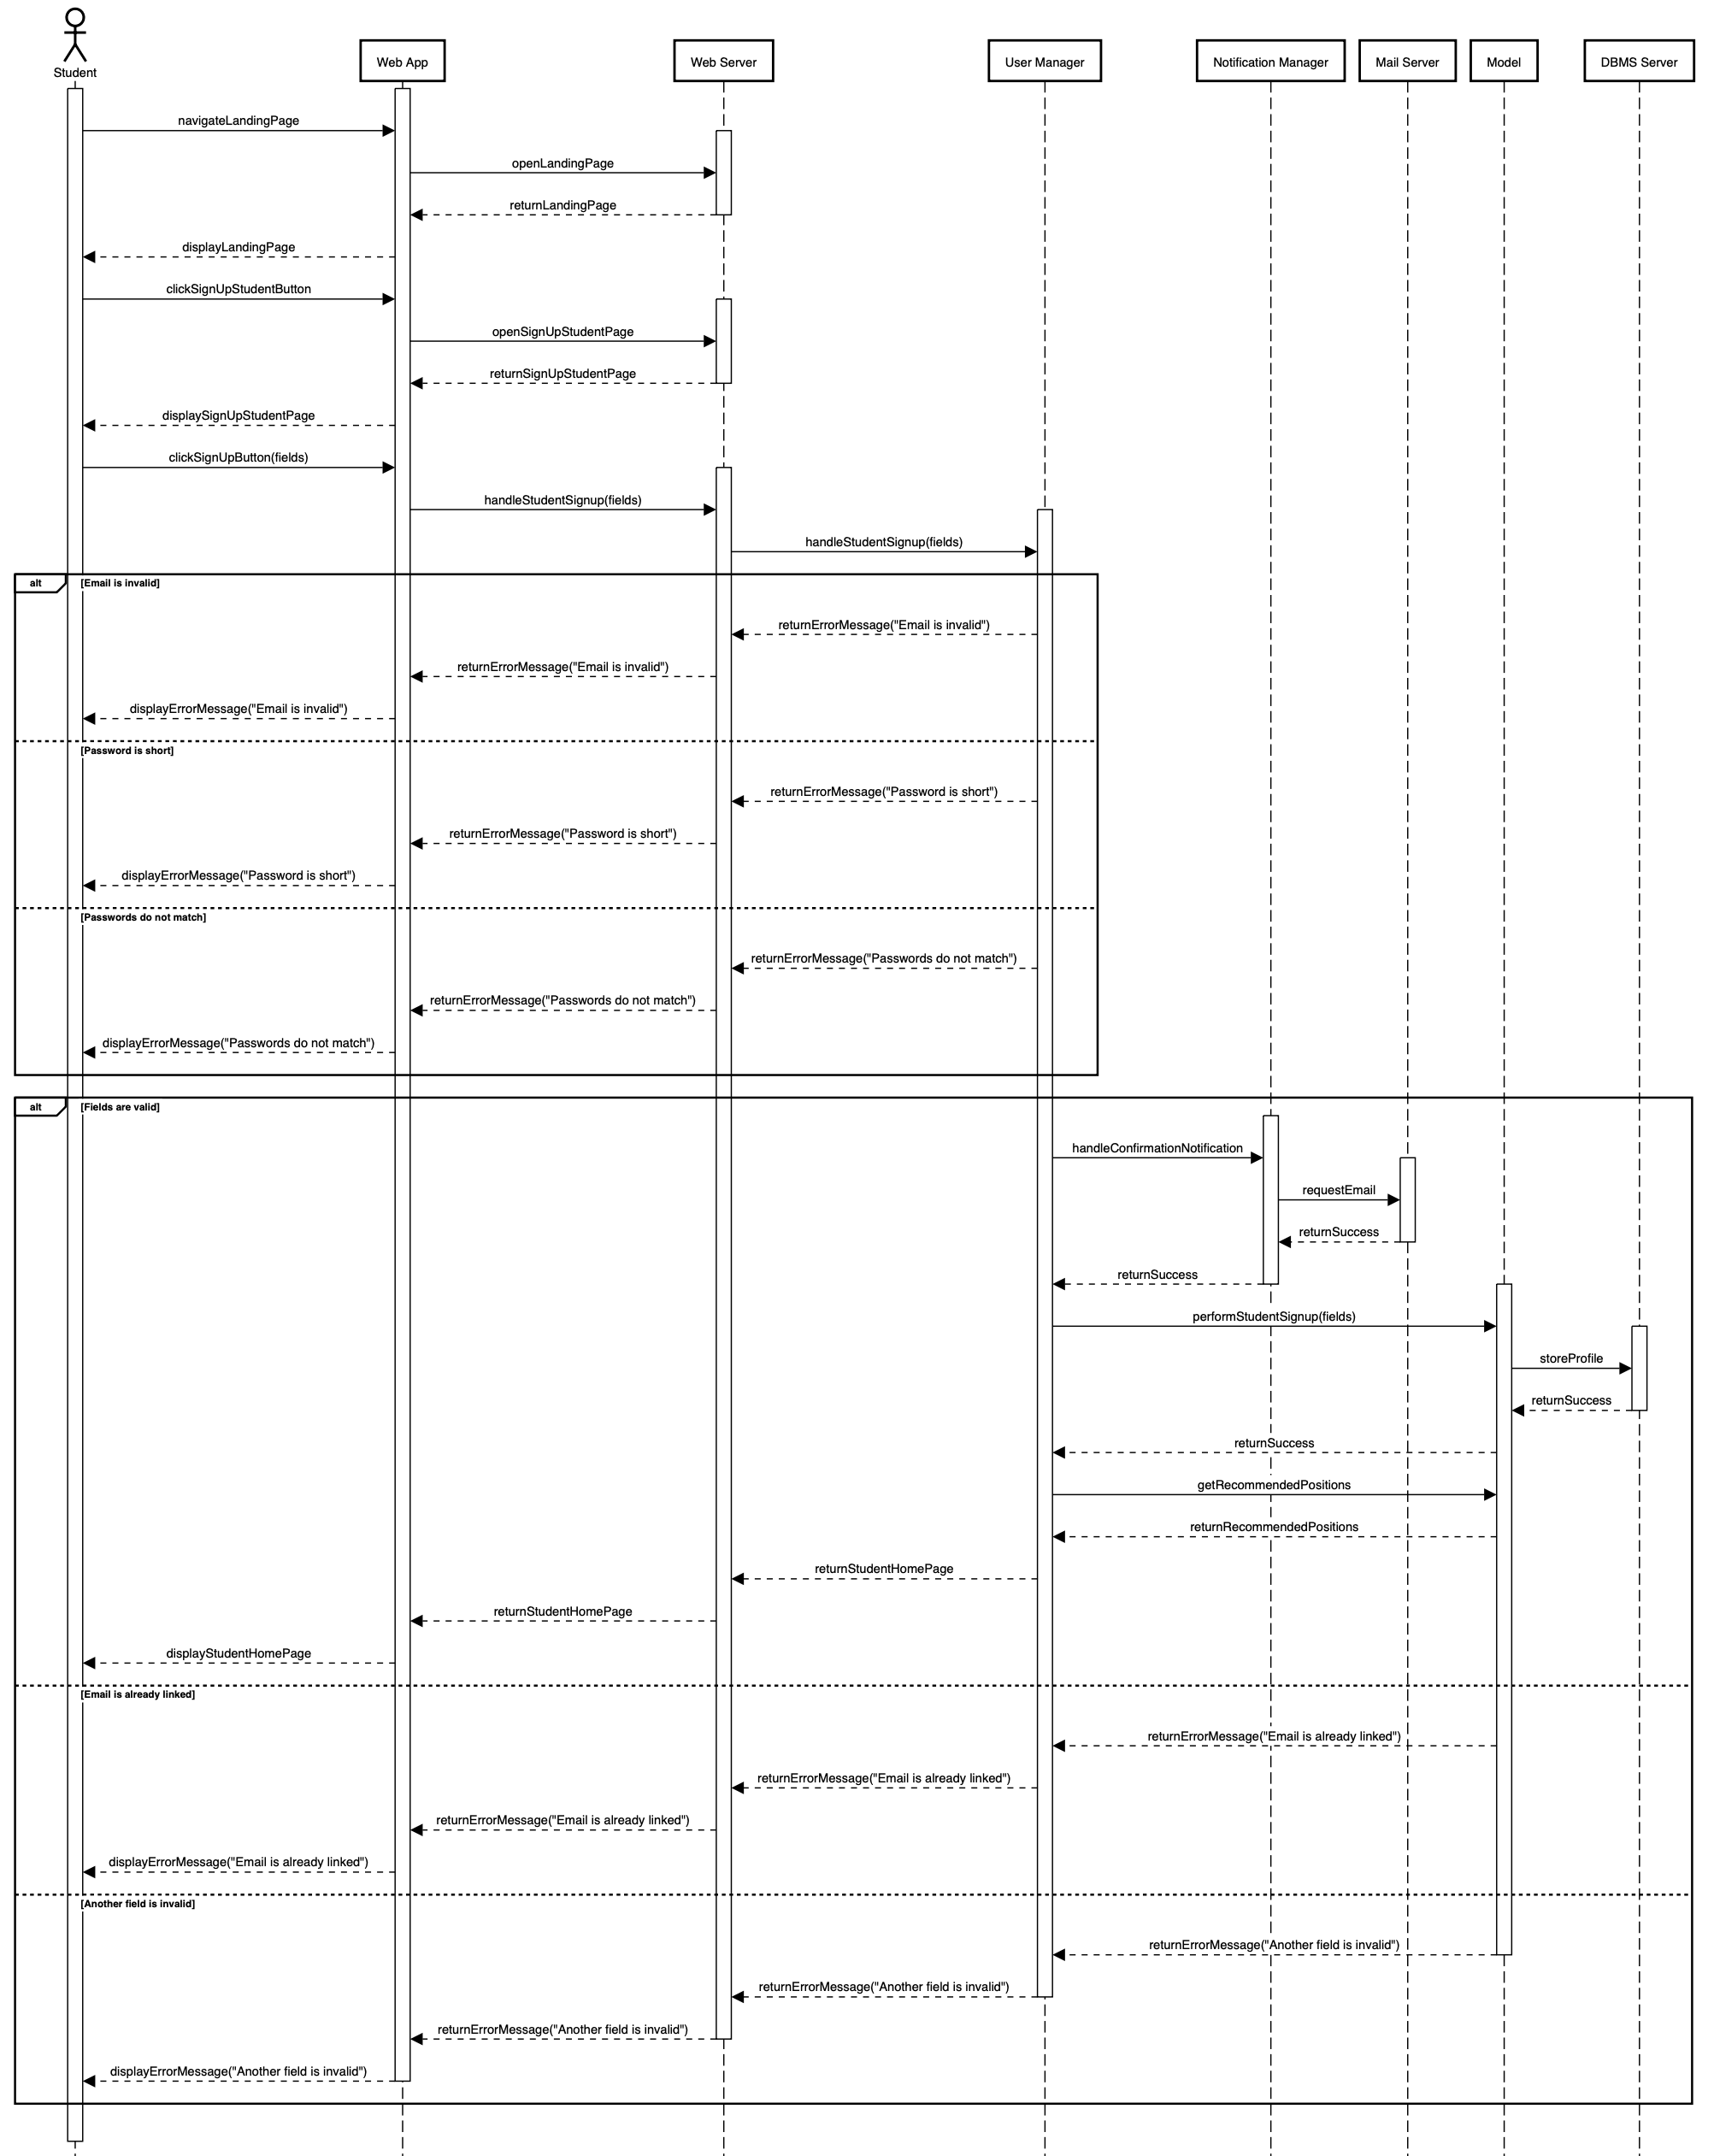
\includegraphics[width=14cm]{images/sequence-diagrams/student-signs-up.png}
    \caption{Student signs up sequence diagram}
\end{figure}

\clearpage
\subsubsection{Student Logs In}
The student is signed up.

\begin{figure}[h]
    \centering
    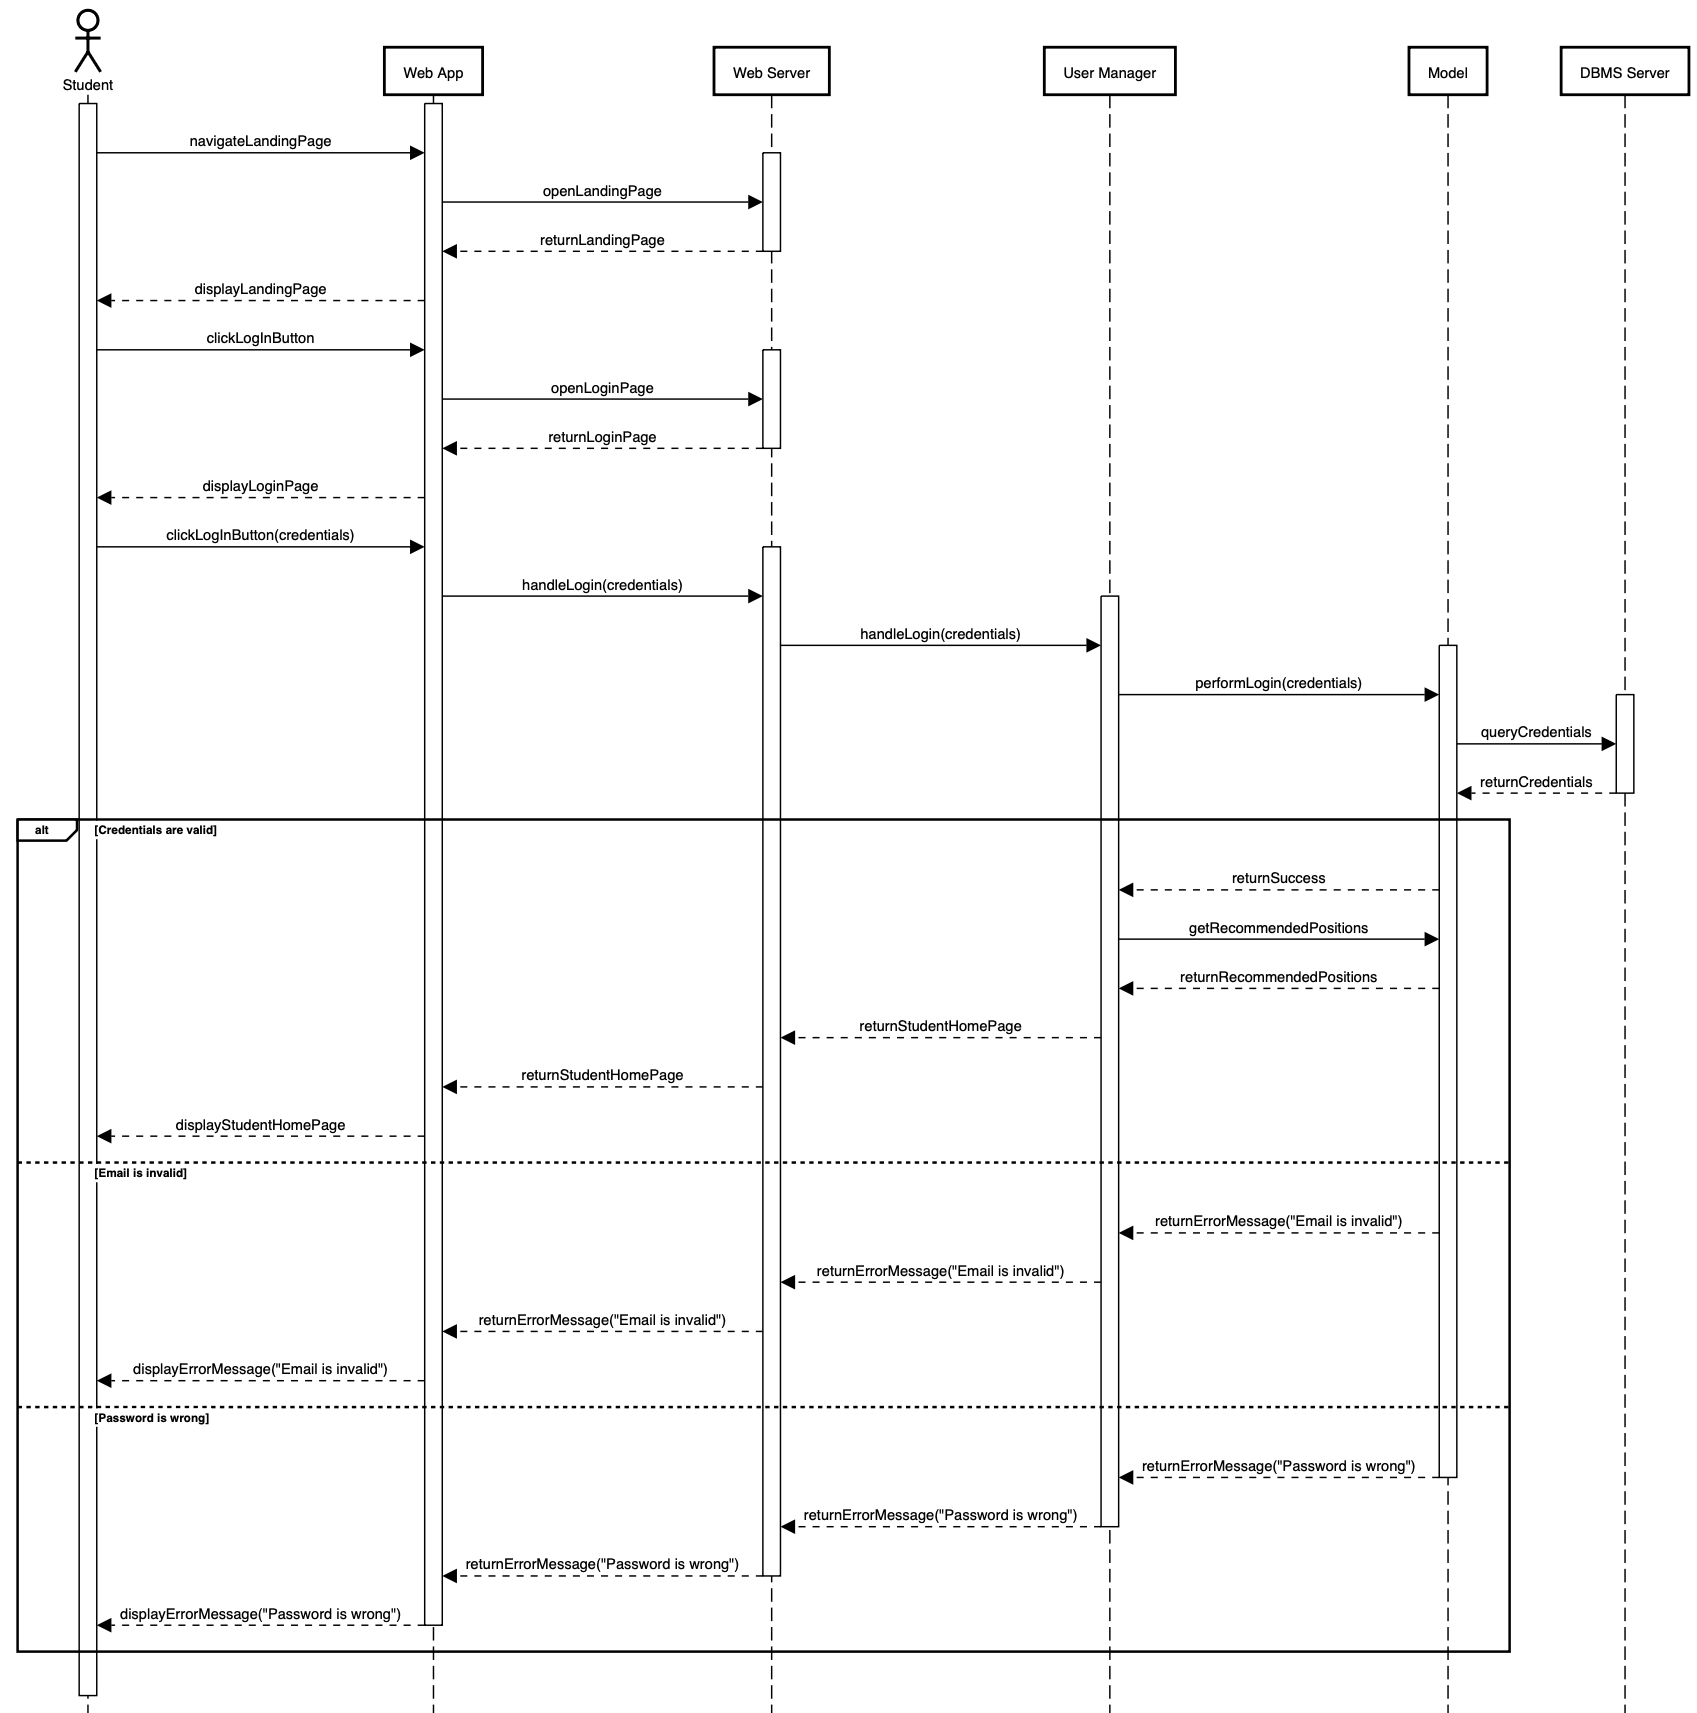
\includegraphics[width=16cm]{images/sequence-diagrams/student-logs-in.png}
    \caption{Student logs in sequence diagram}
\end{figure}

\clearpage
\subsubsection{Student Accepts Recommendation}
The student is logged in, has uploaded a CV, entered preferences and ticked the "Keep Me Updated" field.

\begin{figure}[h]
    \centering
    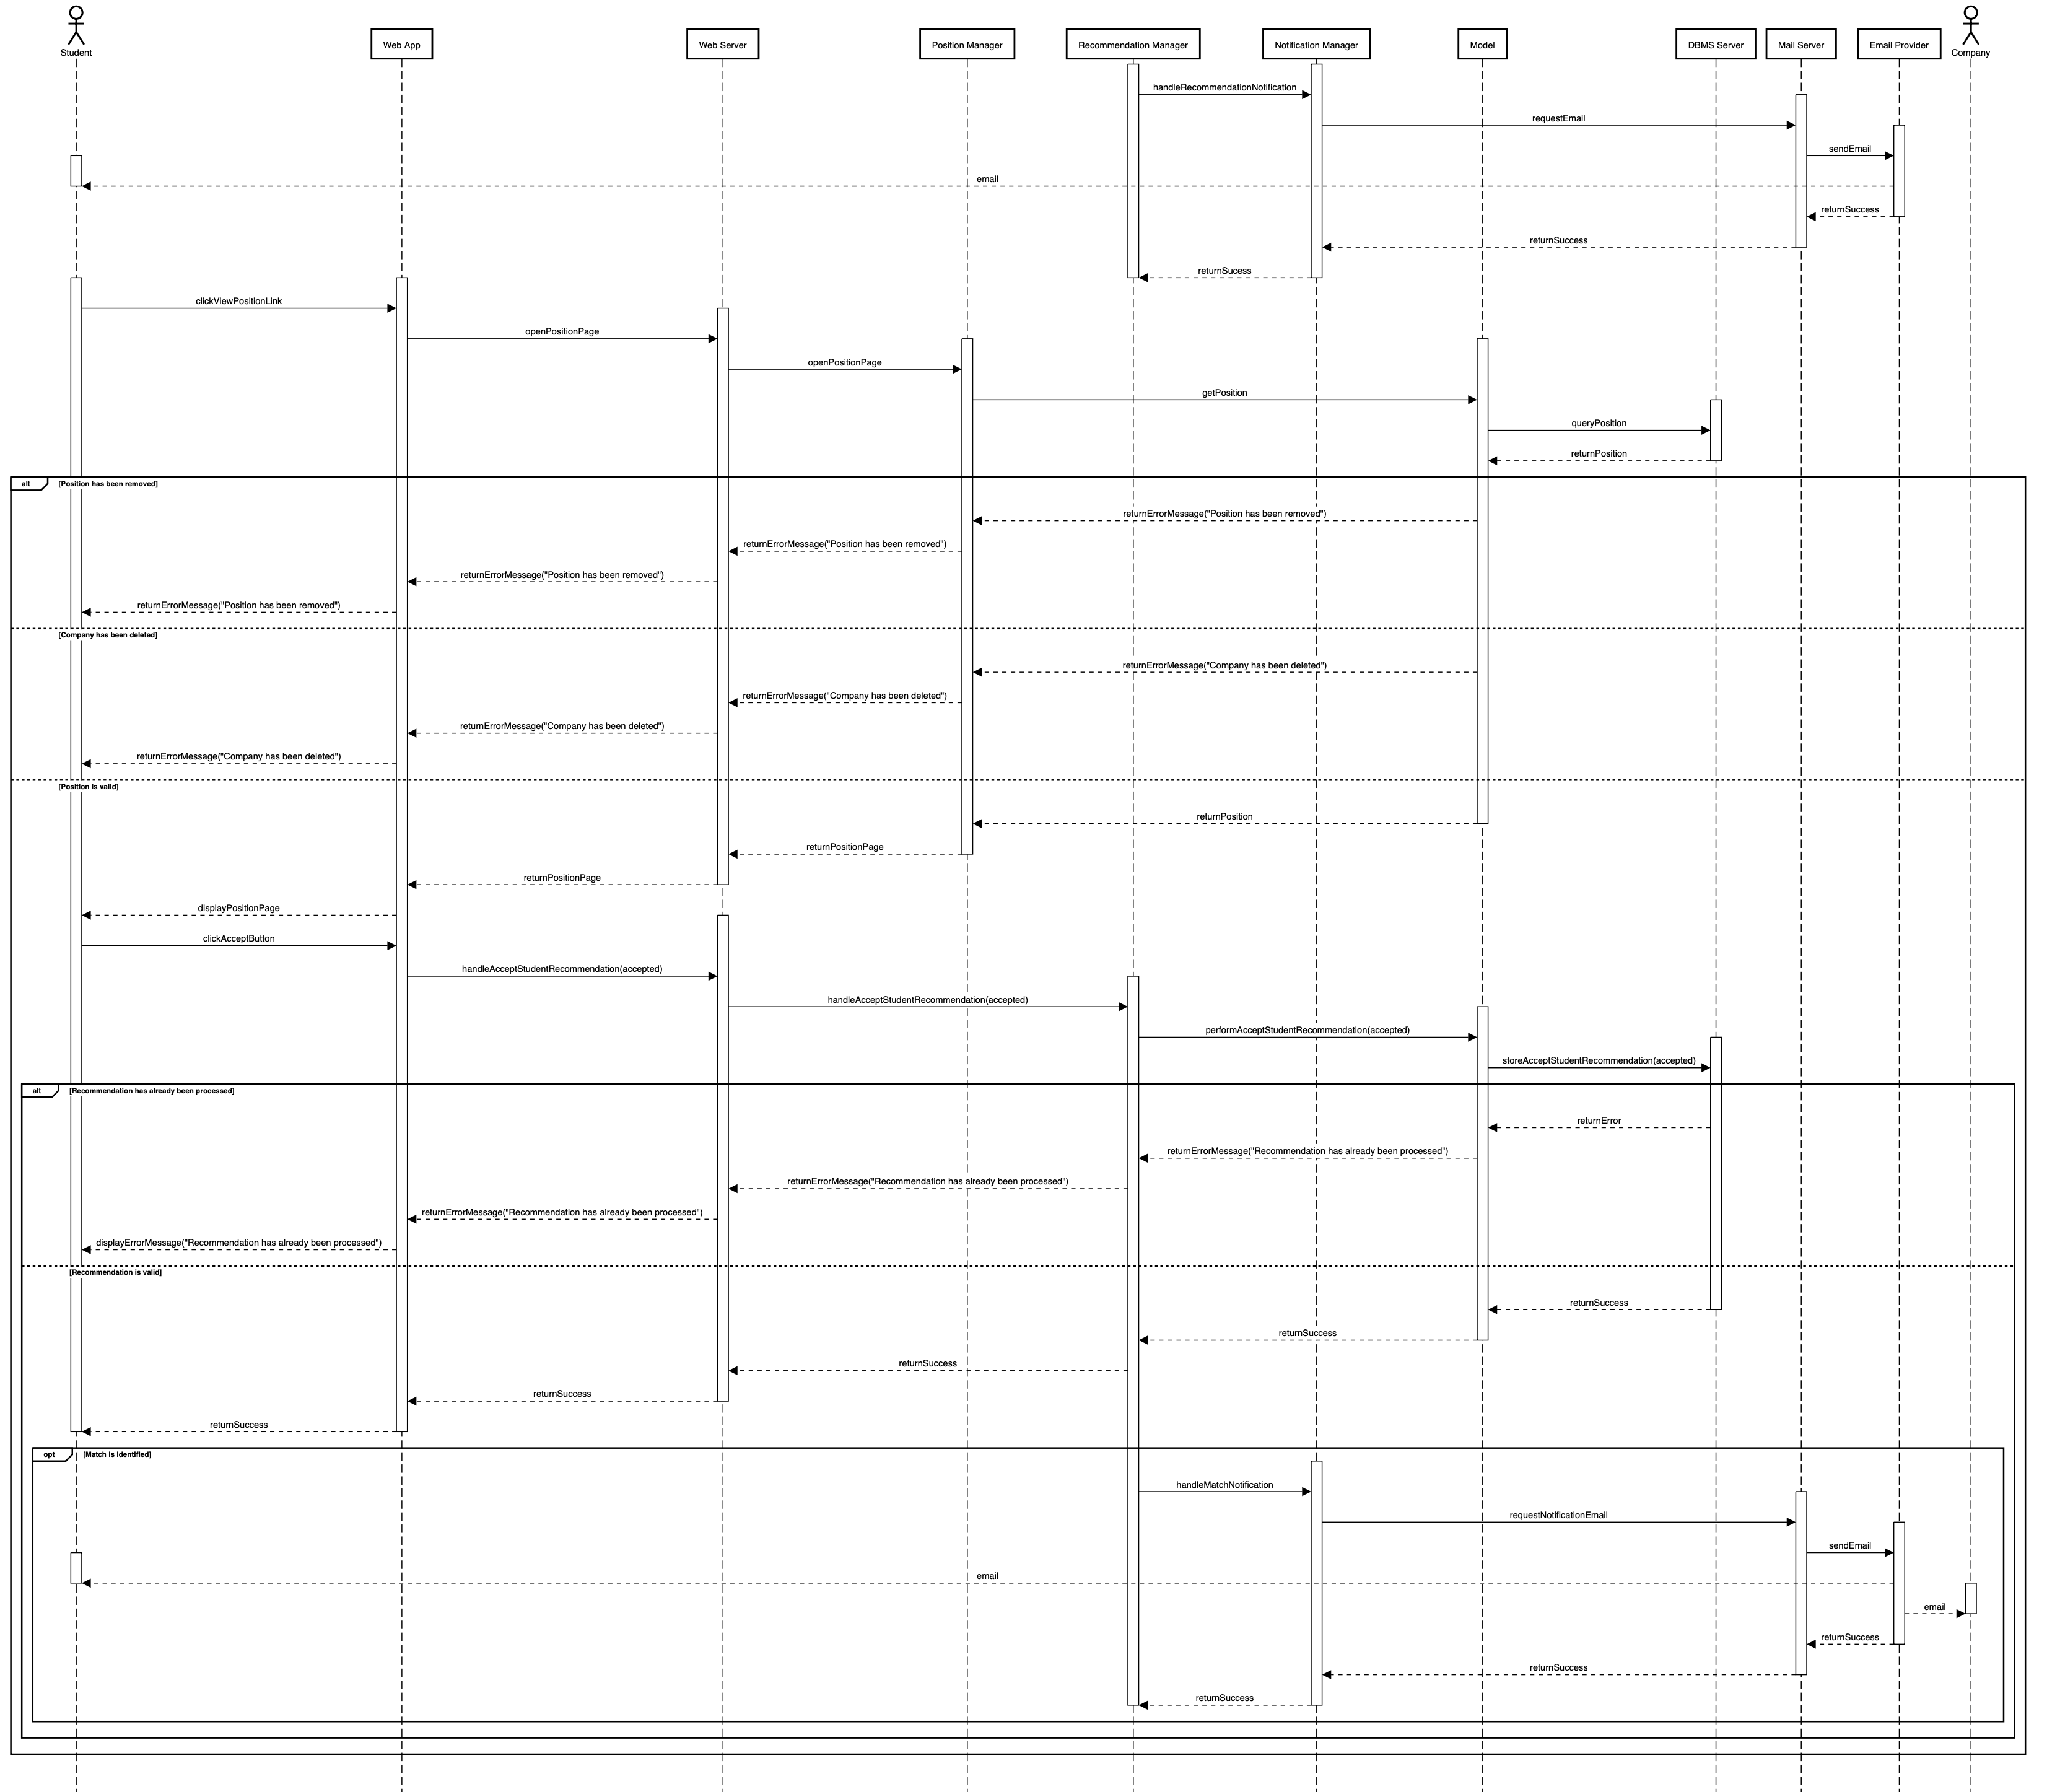
\includegraphics[width=16cm]{images/sequence-diagrams/student-accepts-recommendation.png}
    \caption{Student accepts recommendation sequence diagram}
\end{figure}

\clearpage
\subsubsection{Student Accepts Interview}
The student is logged in, has received a notification on a scheduled interview and he is on the home page.

\begin{figure}[h]
    \centering
    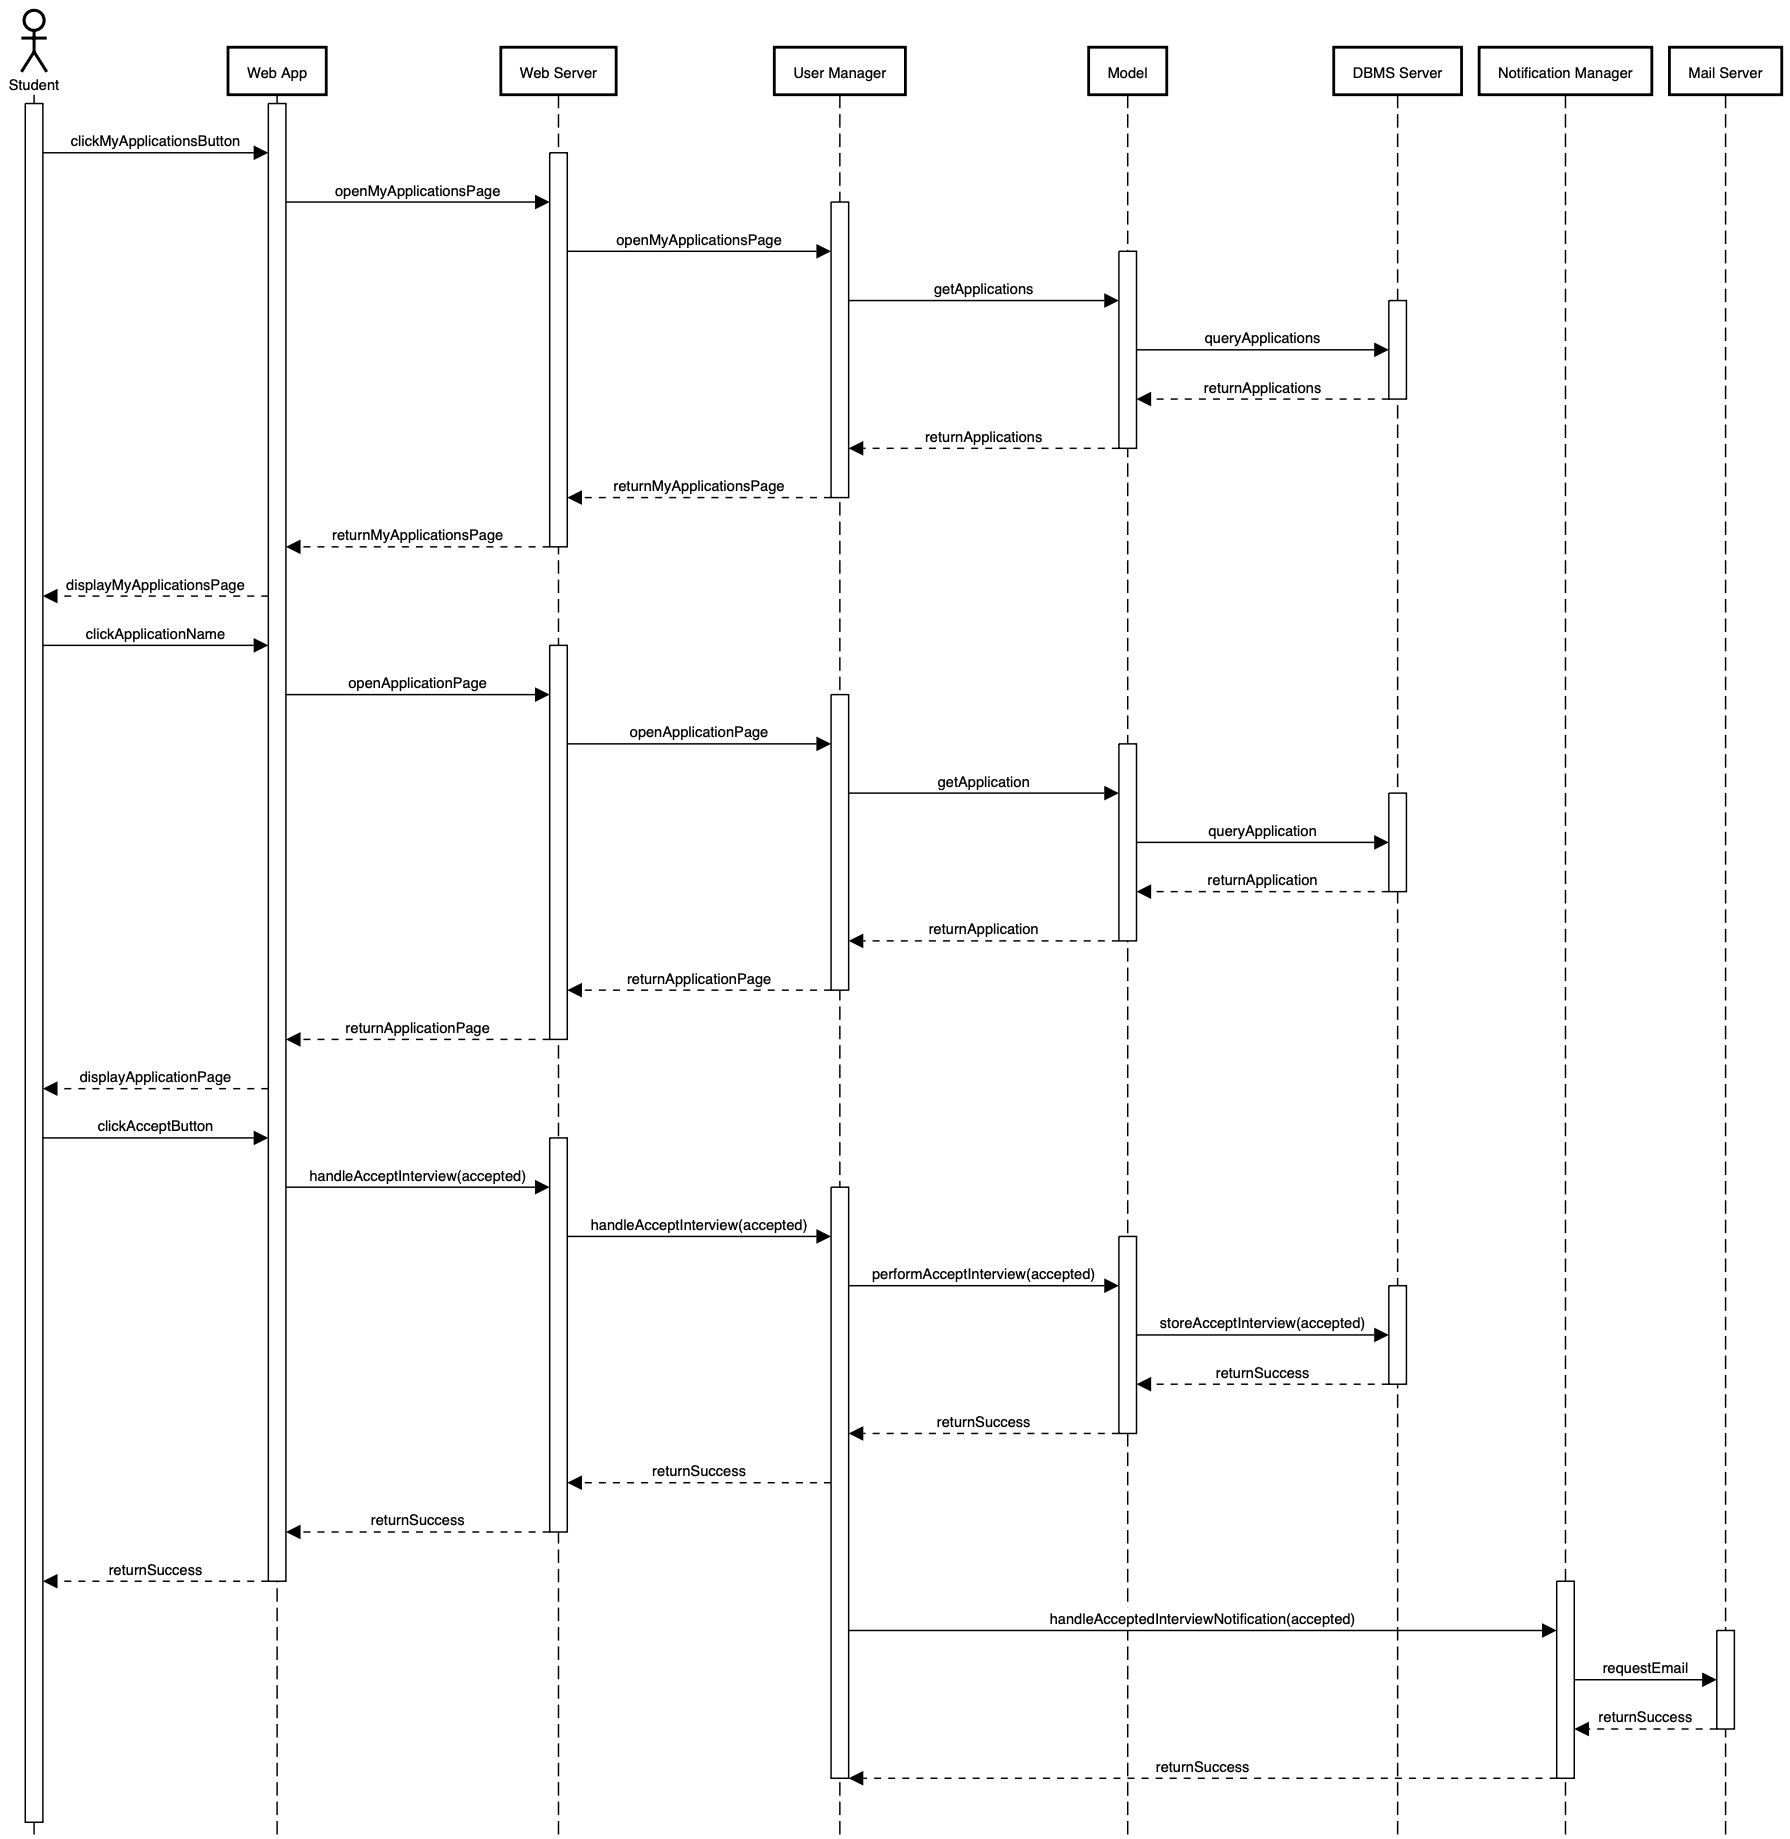
\includegraphics[width=16cm]{images/sequence-diagrams/student-accepts-interview.png}
    \caption{Student accepts interview sequence diagram}
\end{figure}

\clearpage
\subsubsection{Student Comments Internship}
The student is logged in, doing an internship and he is on the home page.

\begin{figure}[h!]
    \centering
    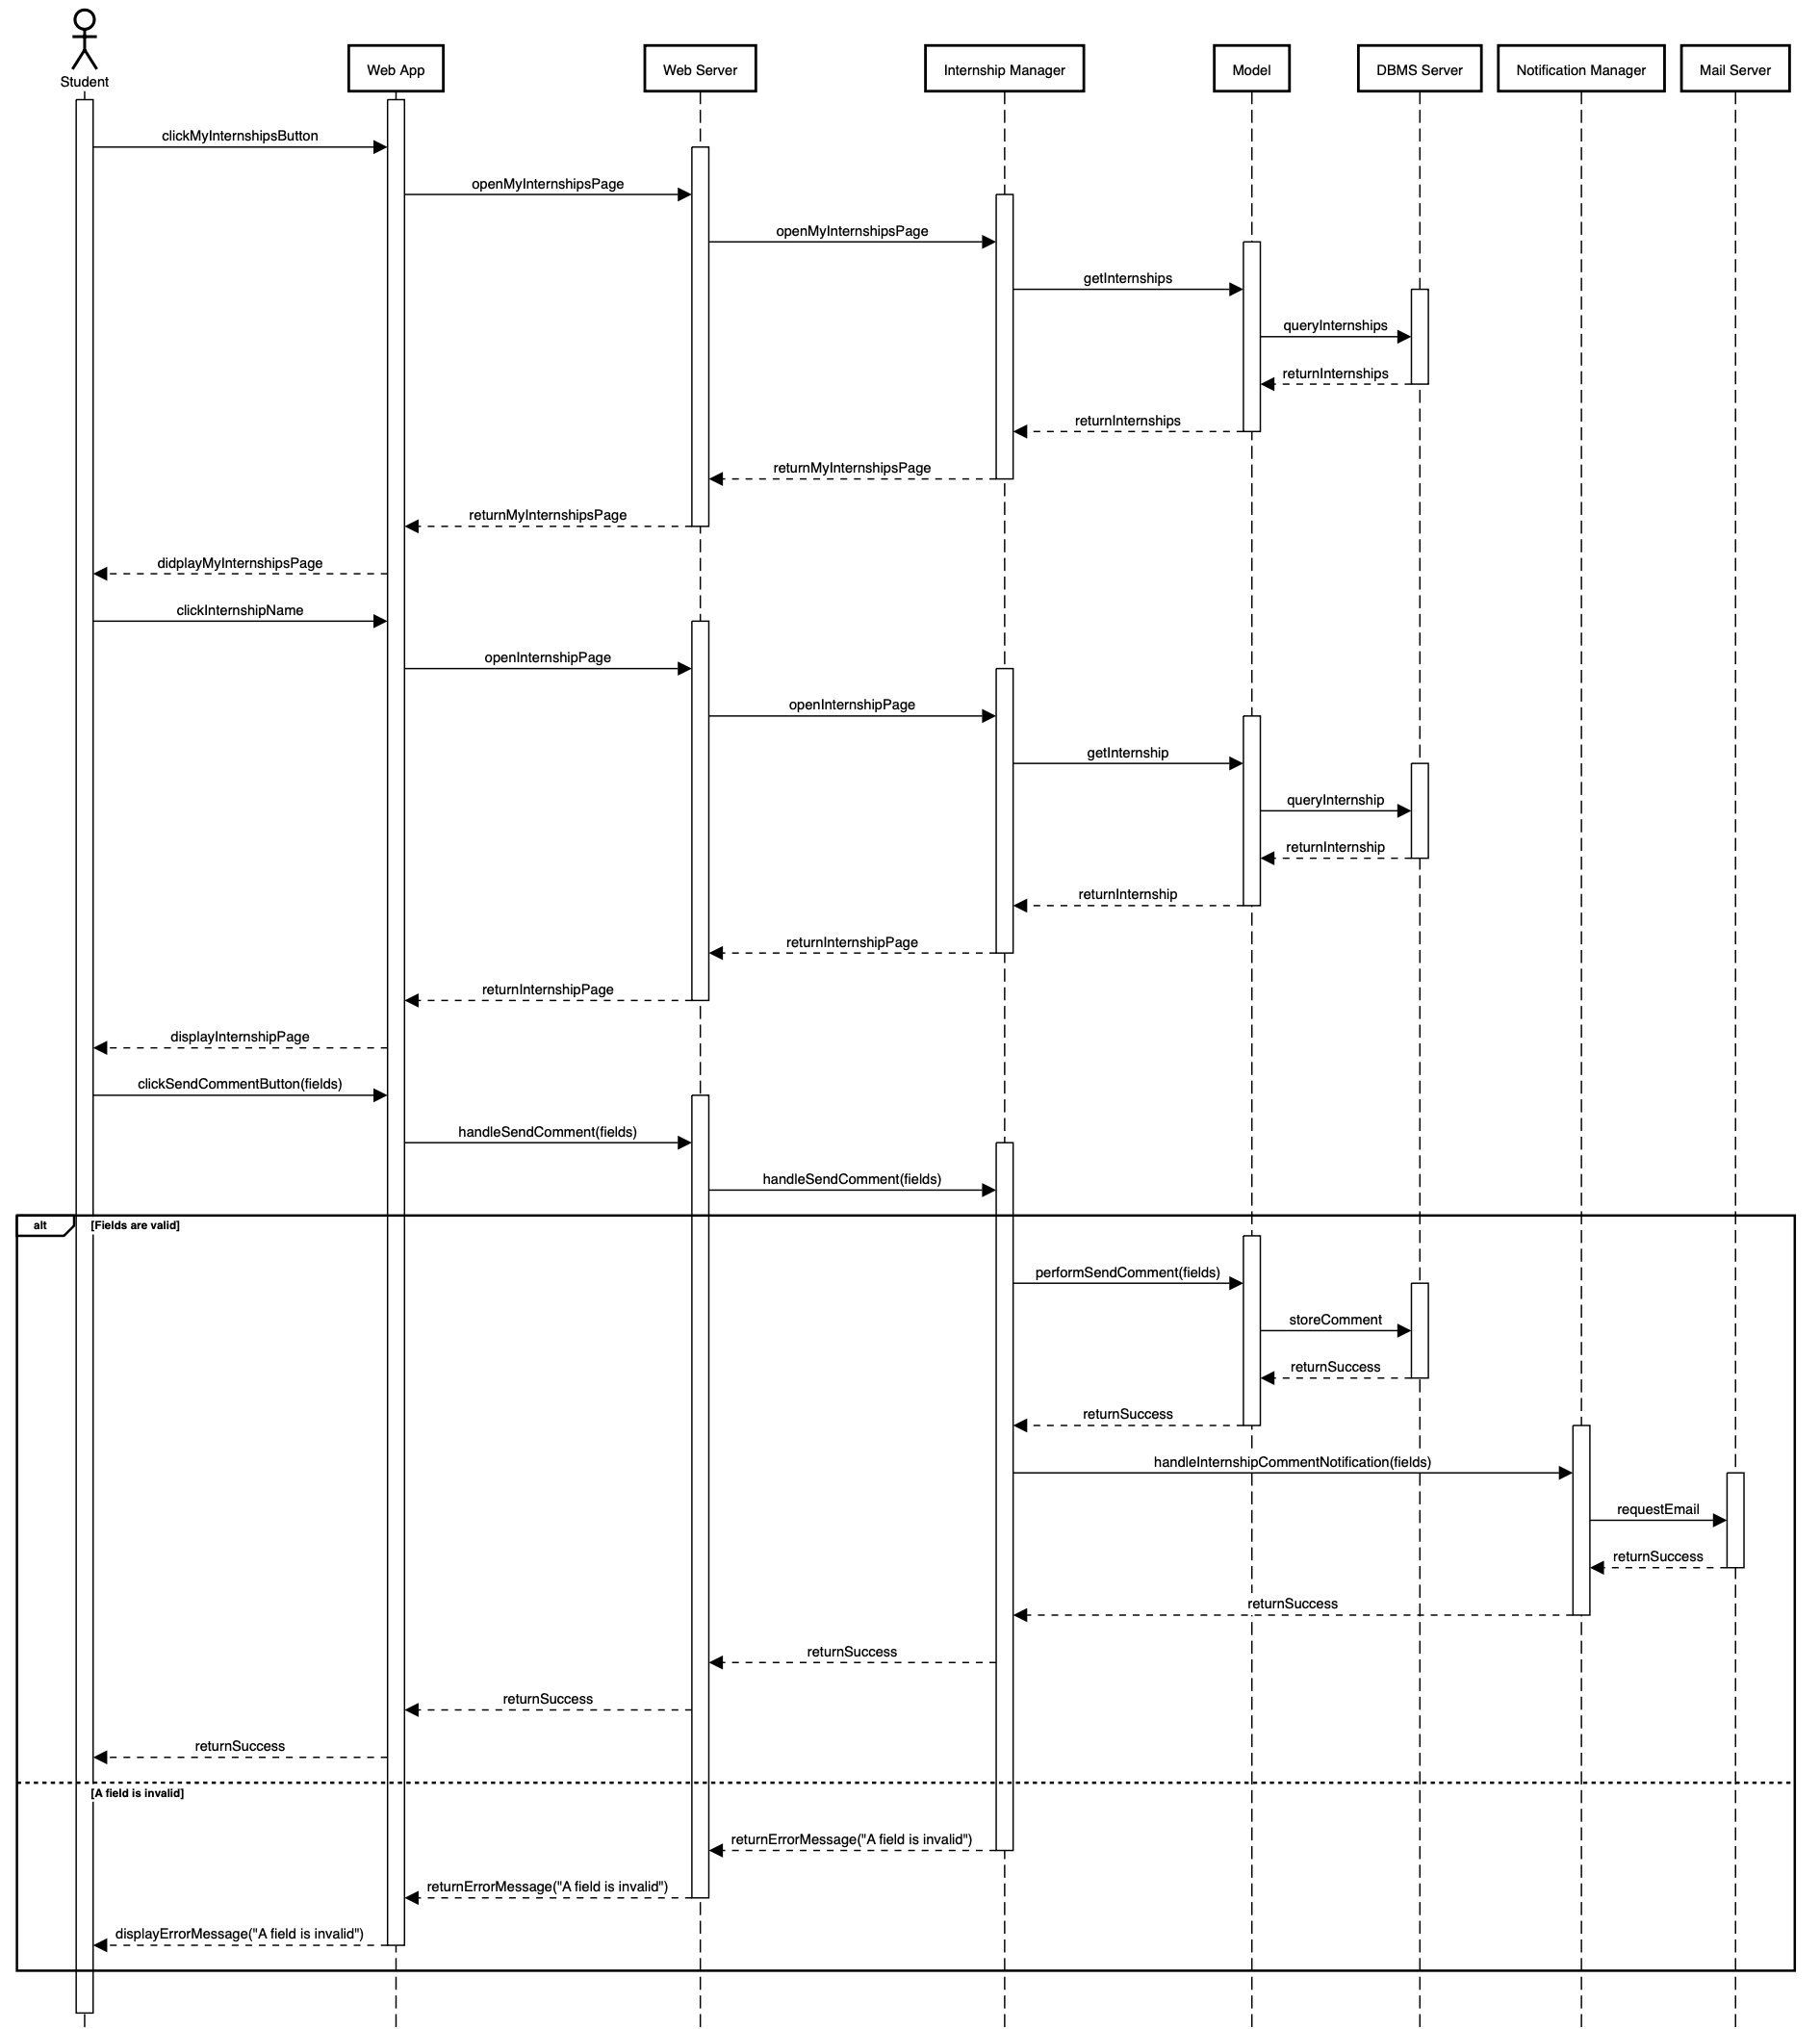
\includegraphics[width=16cm]{images/sequence-diagrams/student-comments-internship.png}
    \caption{Student comments internship sequence diagram}
\end{figure}

\clearpage
\subsection{Company}
\subsubsection{Company Signs Up}
The company is not signed up. 

\begin{figure}[h!]
    \centering
    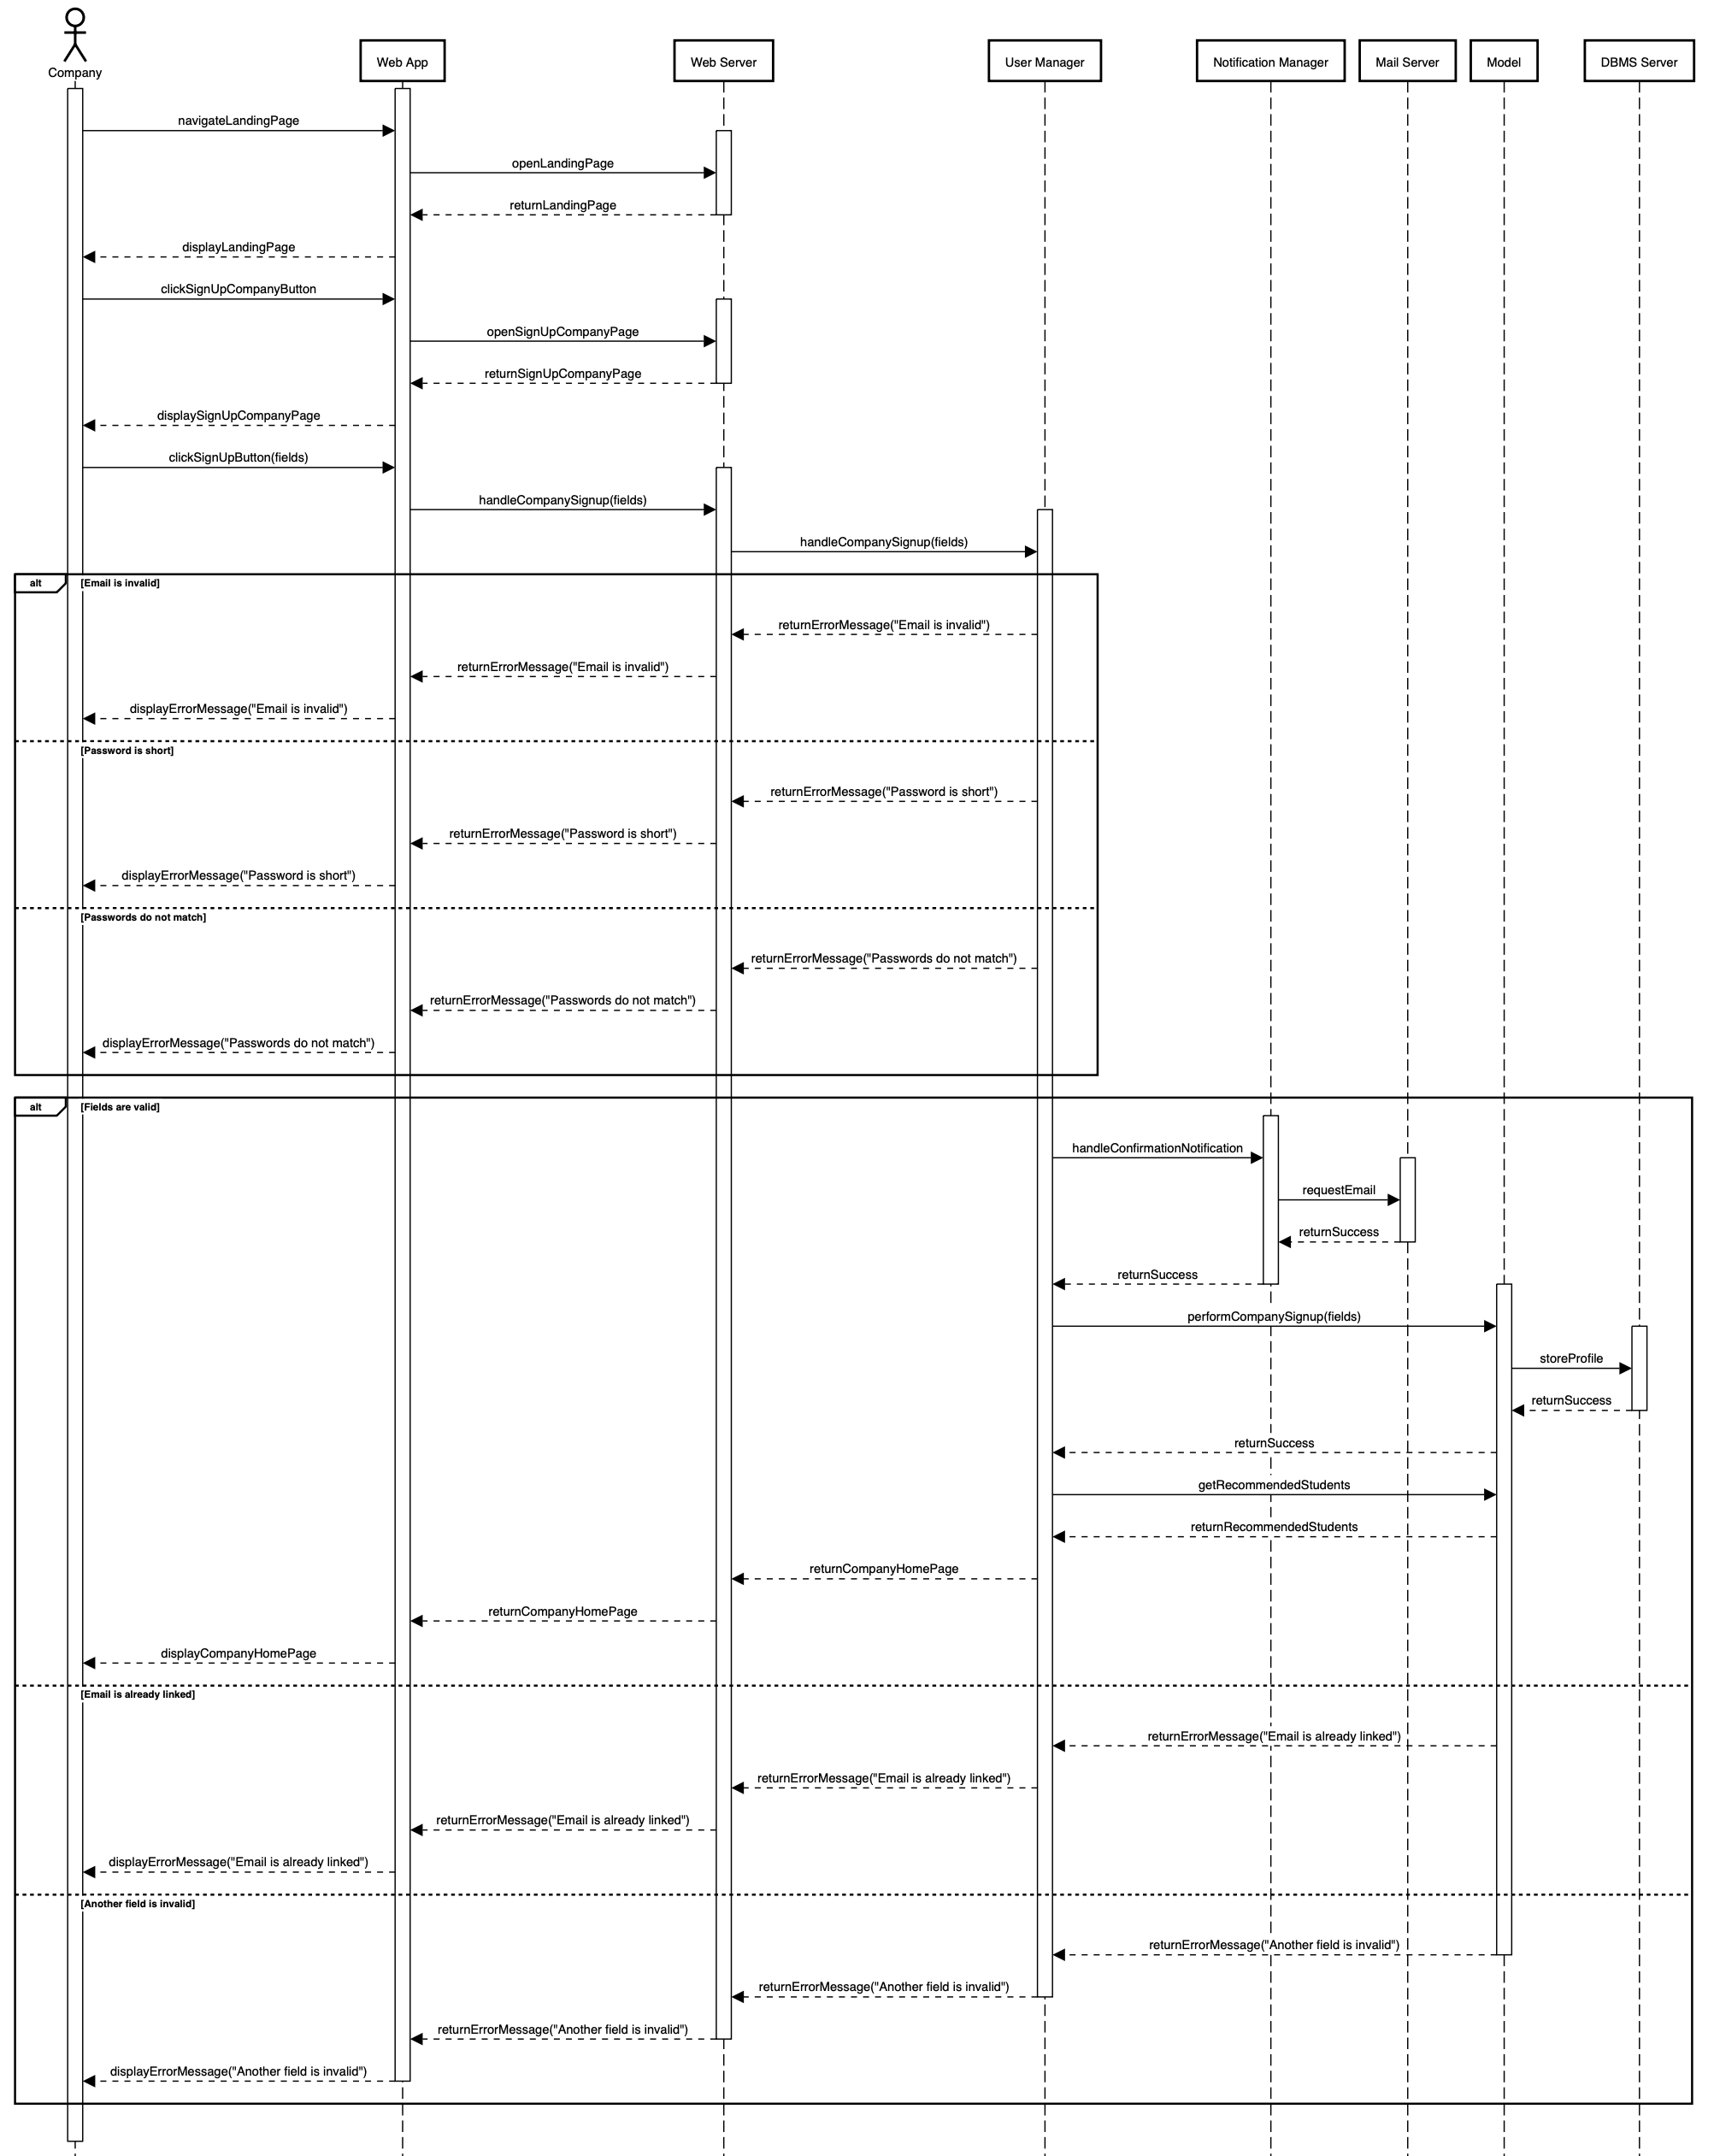
\includegraphics[width=14cm]{images/sequence-diagrams/company-signs-up.png}
    \caption{Company signs up sequence diagram}
\end{figure}

\clearpage
\subsubsection{Company Logs In}
The company is signed up.

\begin{figure}[h]
    \centering
    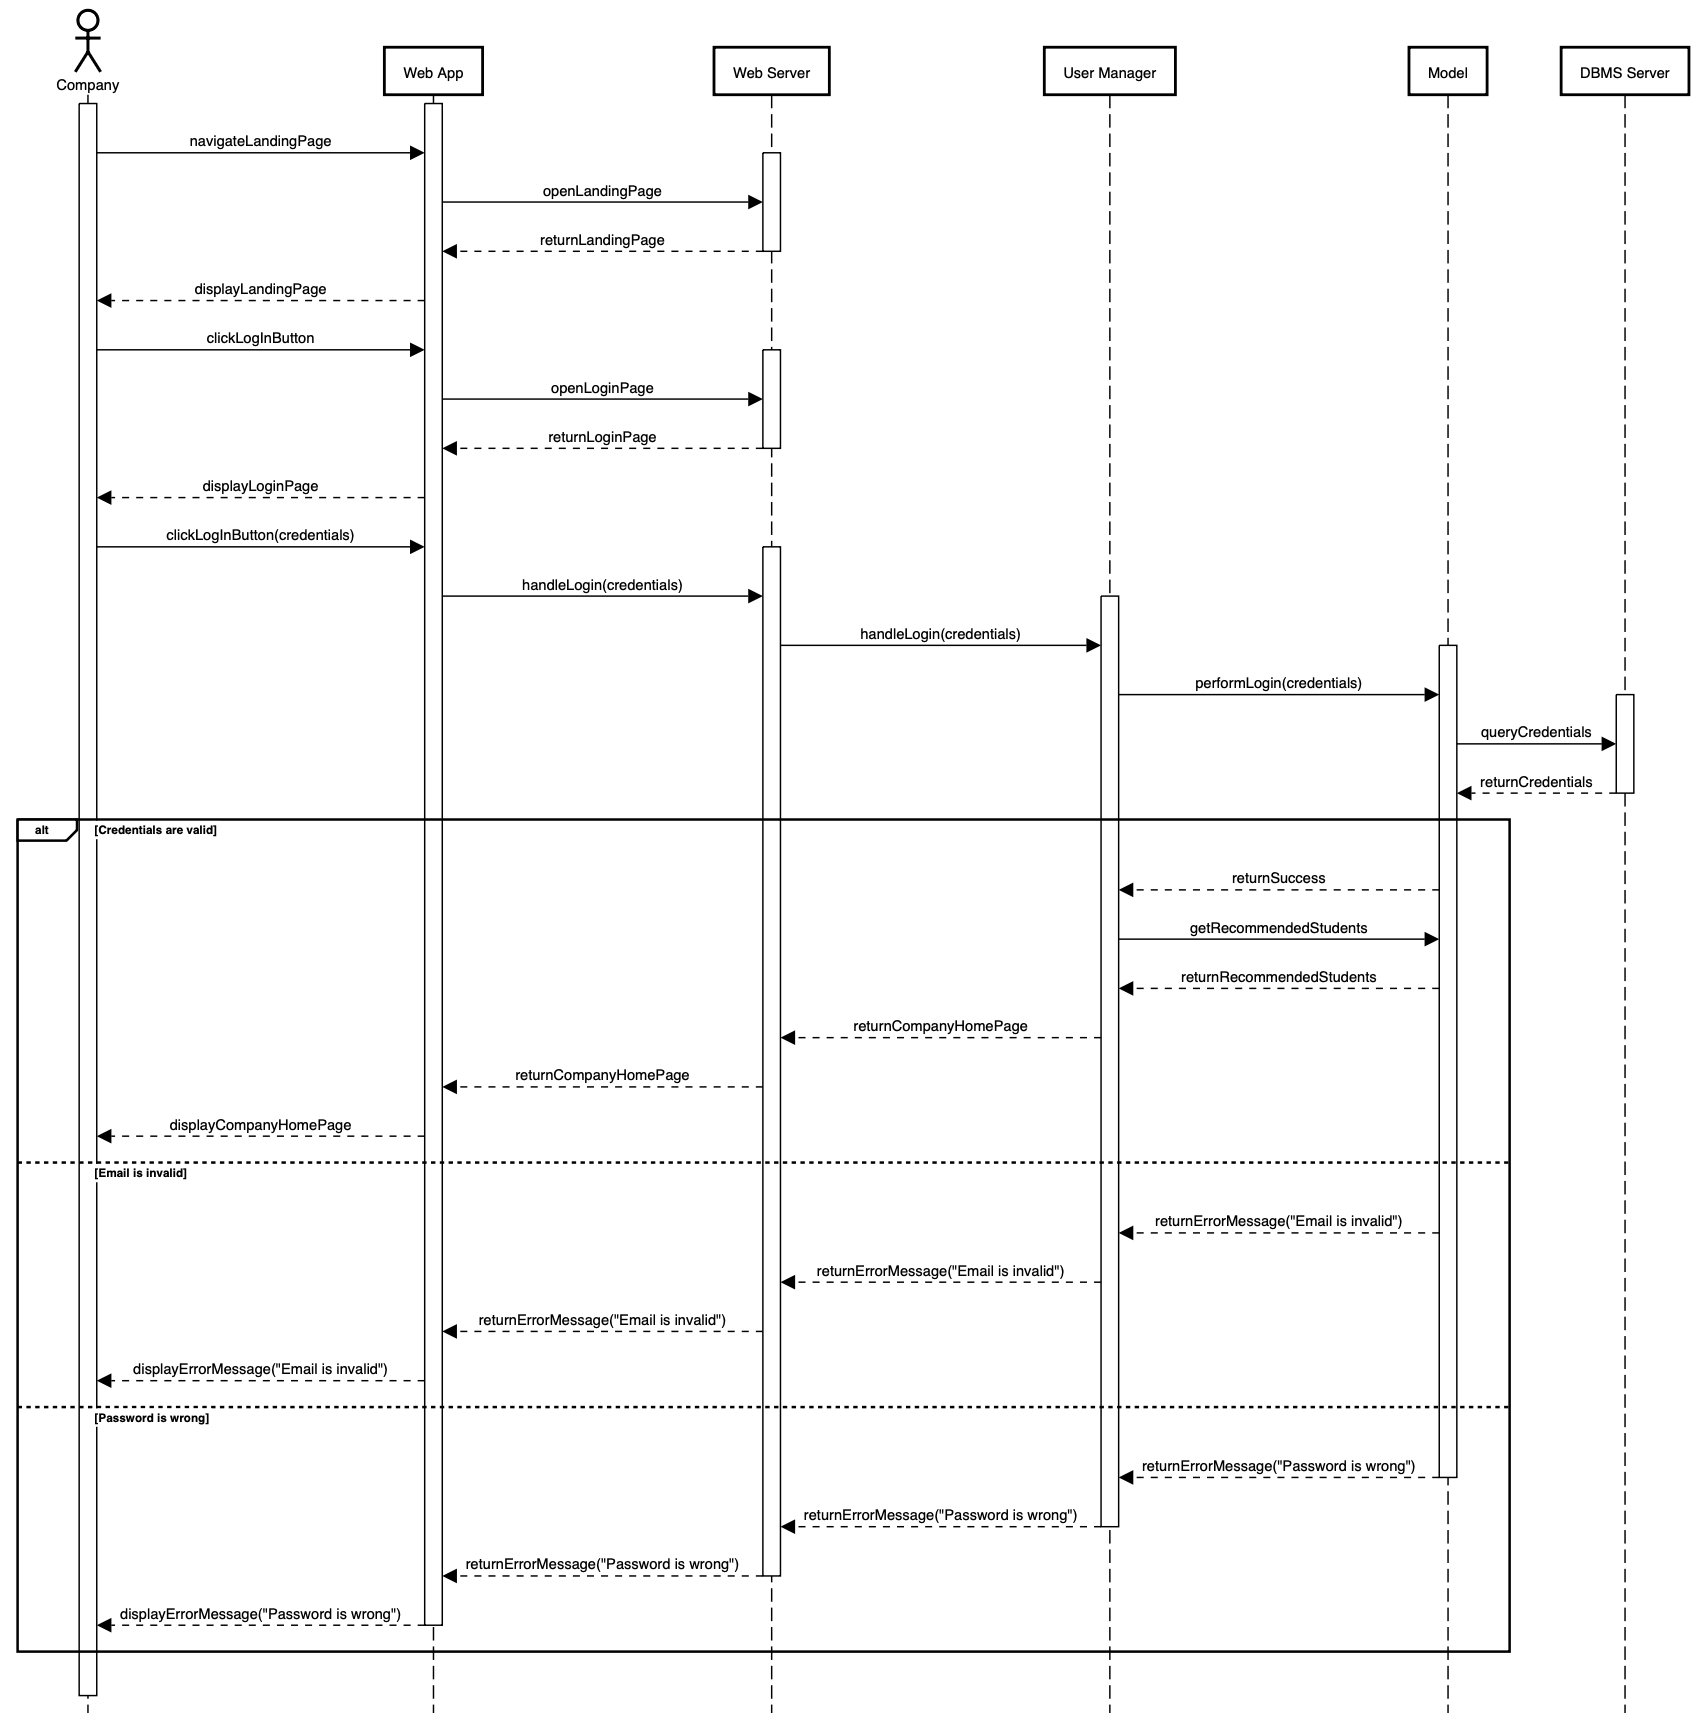
\includegraphics[width=16cm]{images/sequence-diagrams/company-logs-in.png}
    \caption{Company logs in sequence diagram}
\end{figure}

\clearpage
\subsubsection{Company Accepts Recommendation}
The company is logged in, has posted a position and has ticked the "Keep Me Updated" field.

\begin{figure}[h]
    \centering
    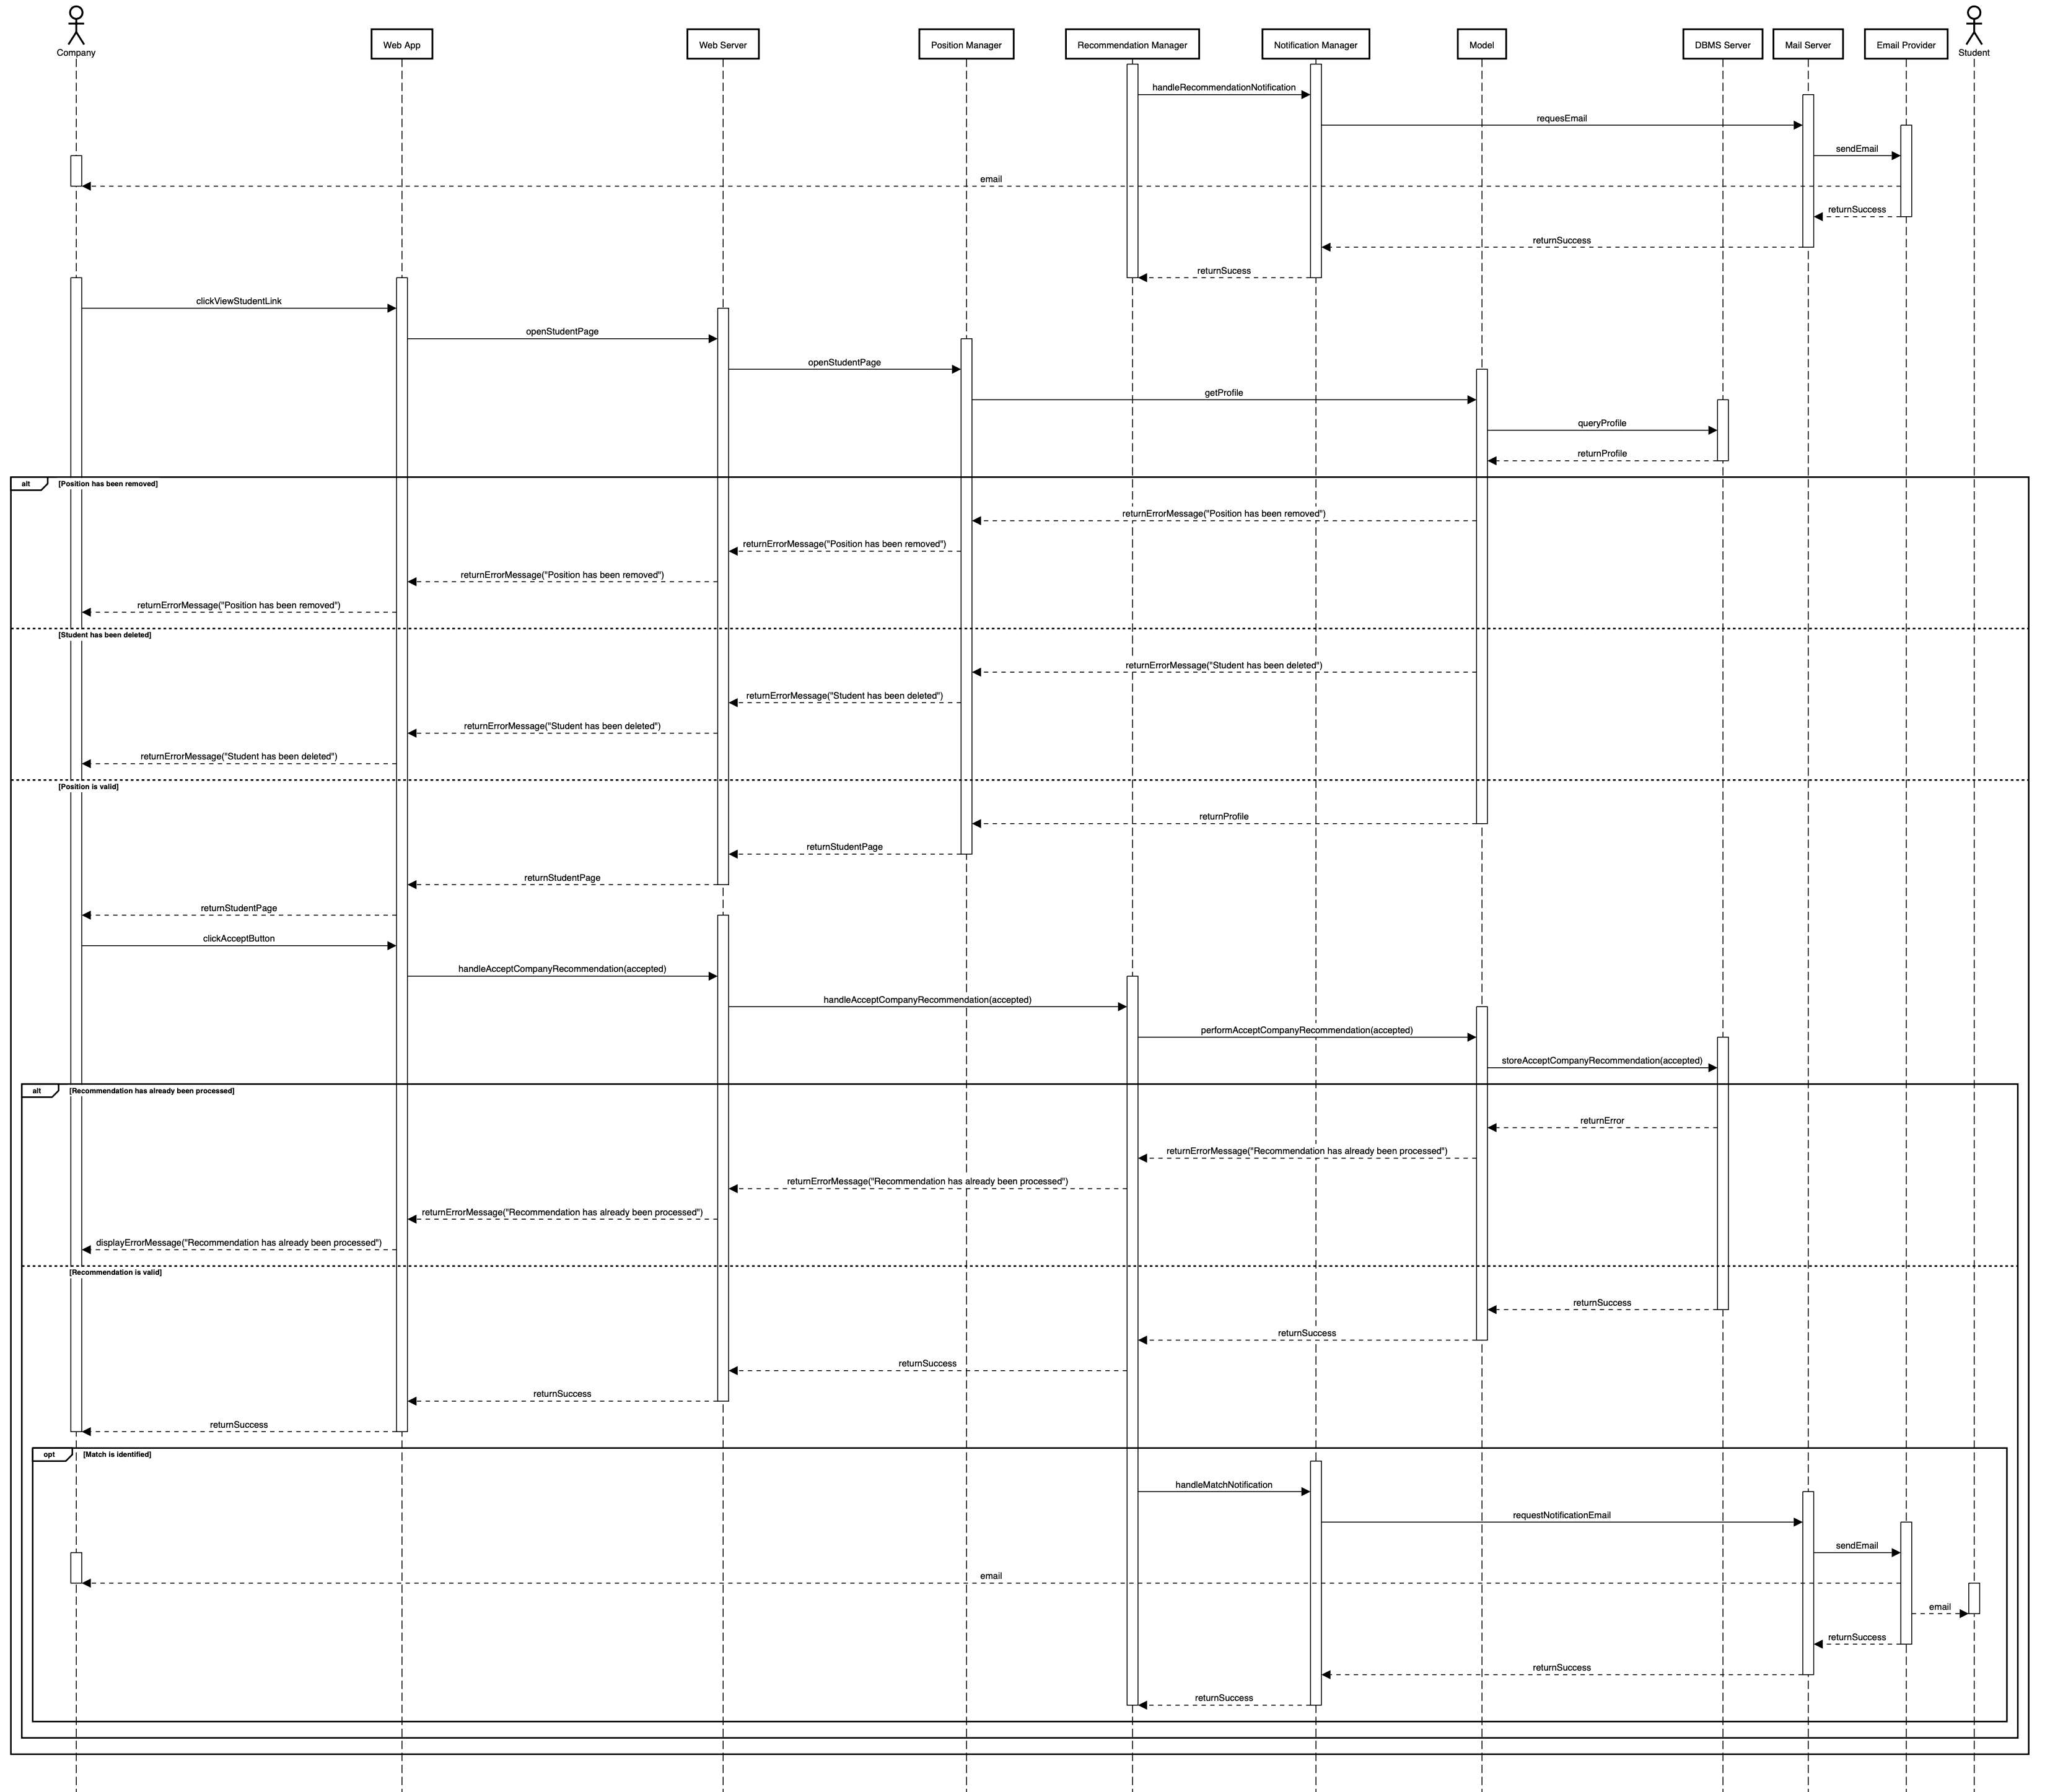
\includegraphics[width=16cm]{images/sequence-diagrams/company-accepts-recommendation.png}
    \caption{Company accepts recommendation sequence diagram}
\end{figure}

\clearpage
\subsubsection{Company Schedules Interview}
The company is logged in, has posted a position and it is on the home page.

\begin{figure}[h!]
    \centering
    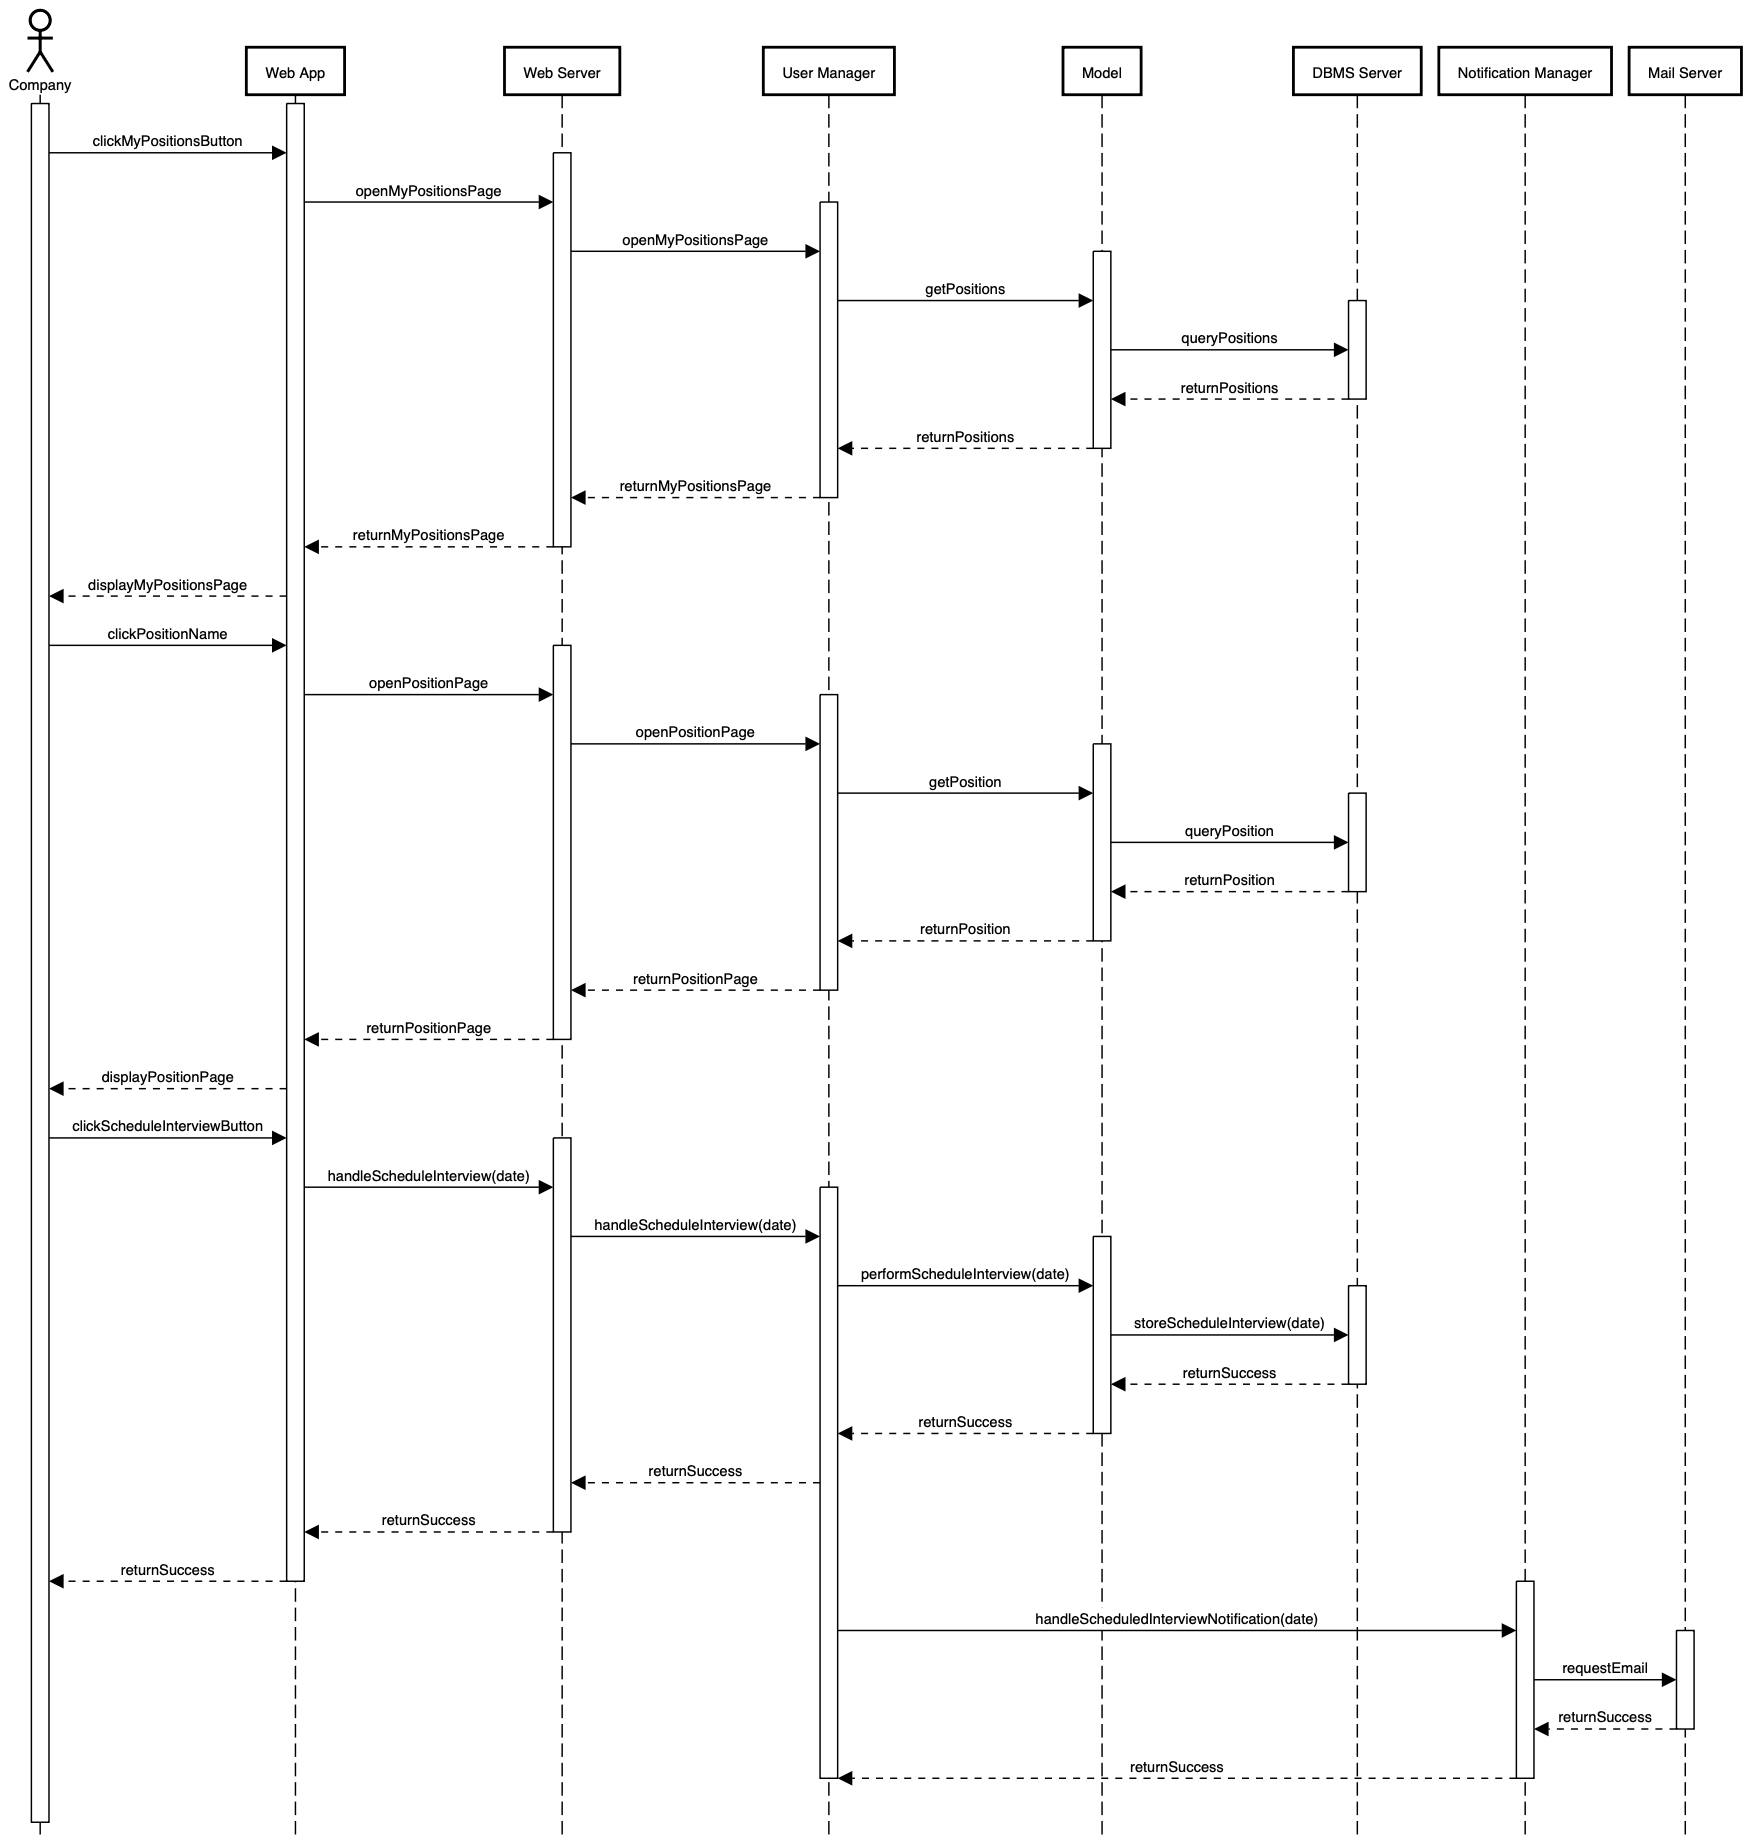
\includegraphics[width=14cm]{images/sequence-diagrams/company-schedules-interview.png}
    \caption{Company schedules interview sequence diagram}
\end{figure}

\clearpage
\subsubsection{Company Comments Internship}
The company is logged in, hosting an internship and it is on the home page.

\begin{figure}[h!] 
    \centering
    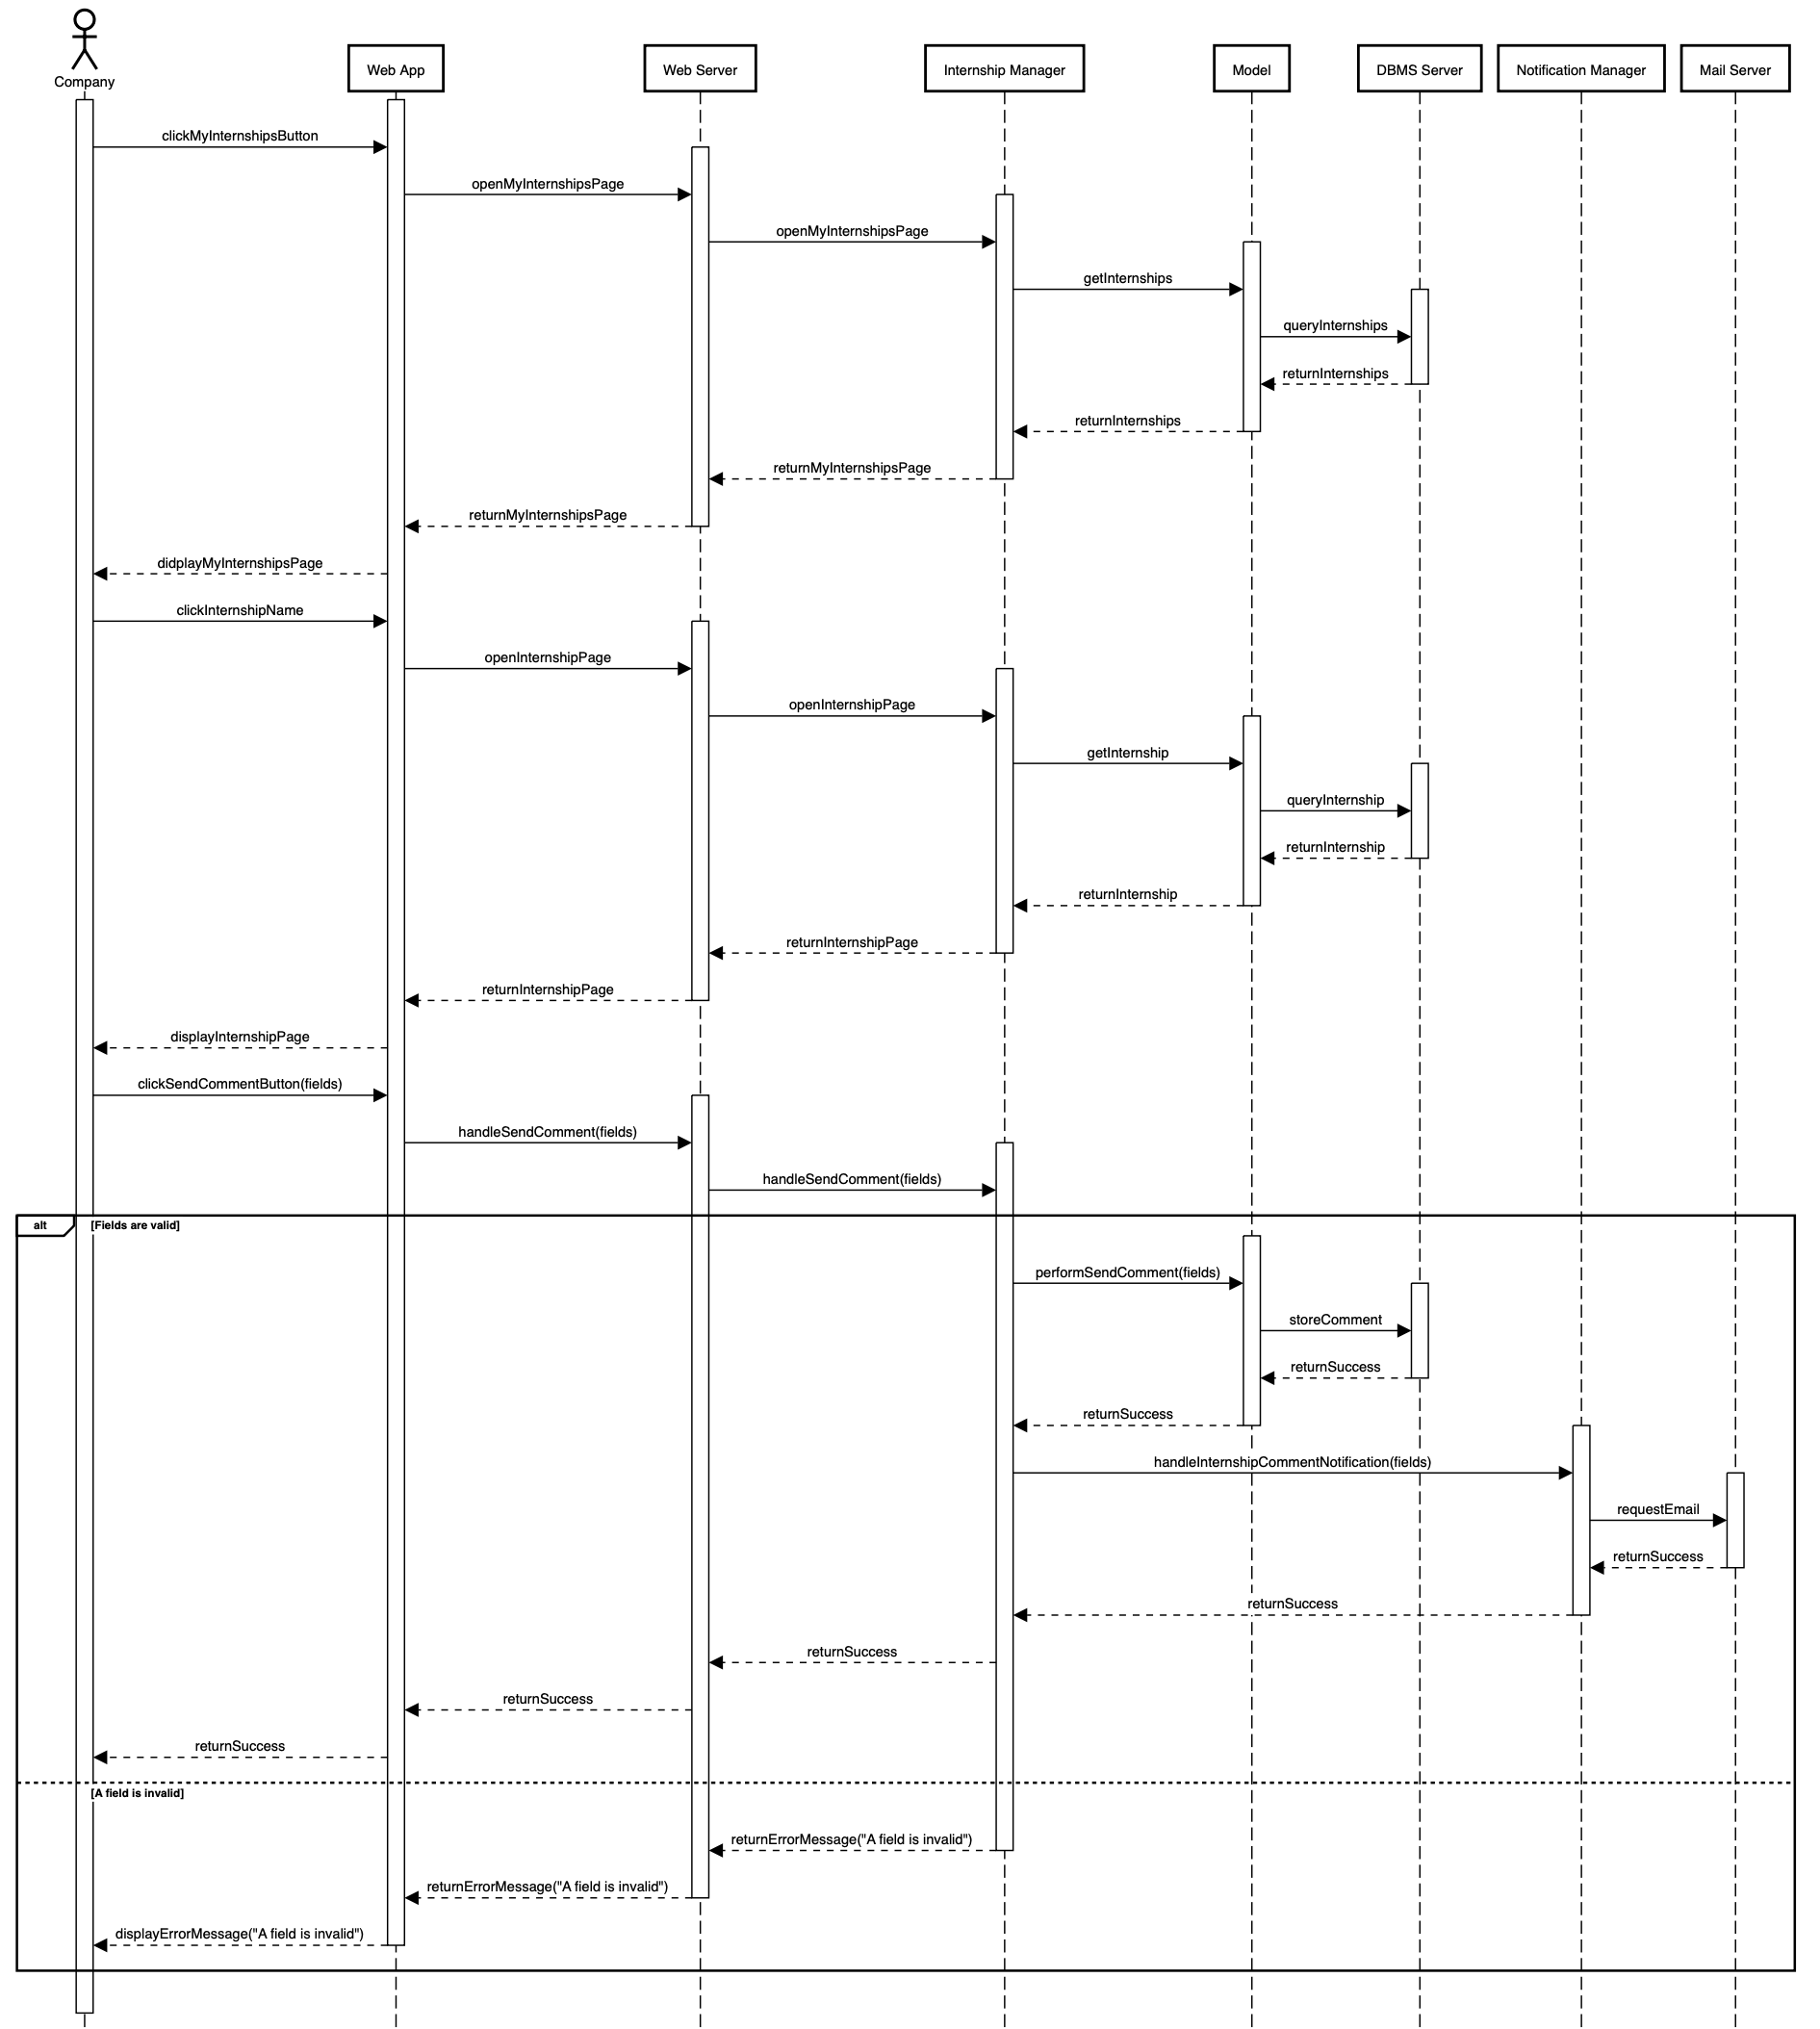
\includegraphics[width=16cm]{images/sequence-diagrams/company-comments-internship.png}
    \caption{Company comments internship sequence diagram}
\end{figure}

\clearpage
\subsection{University}
\subsubsection{University Signs Up}
The university is not signed up.

\begin{figure}[h!]
    \centering
    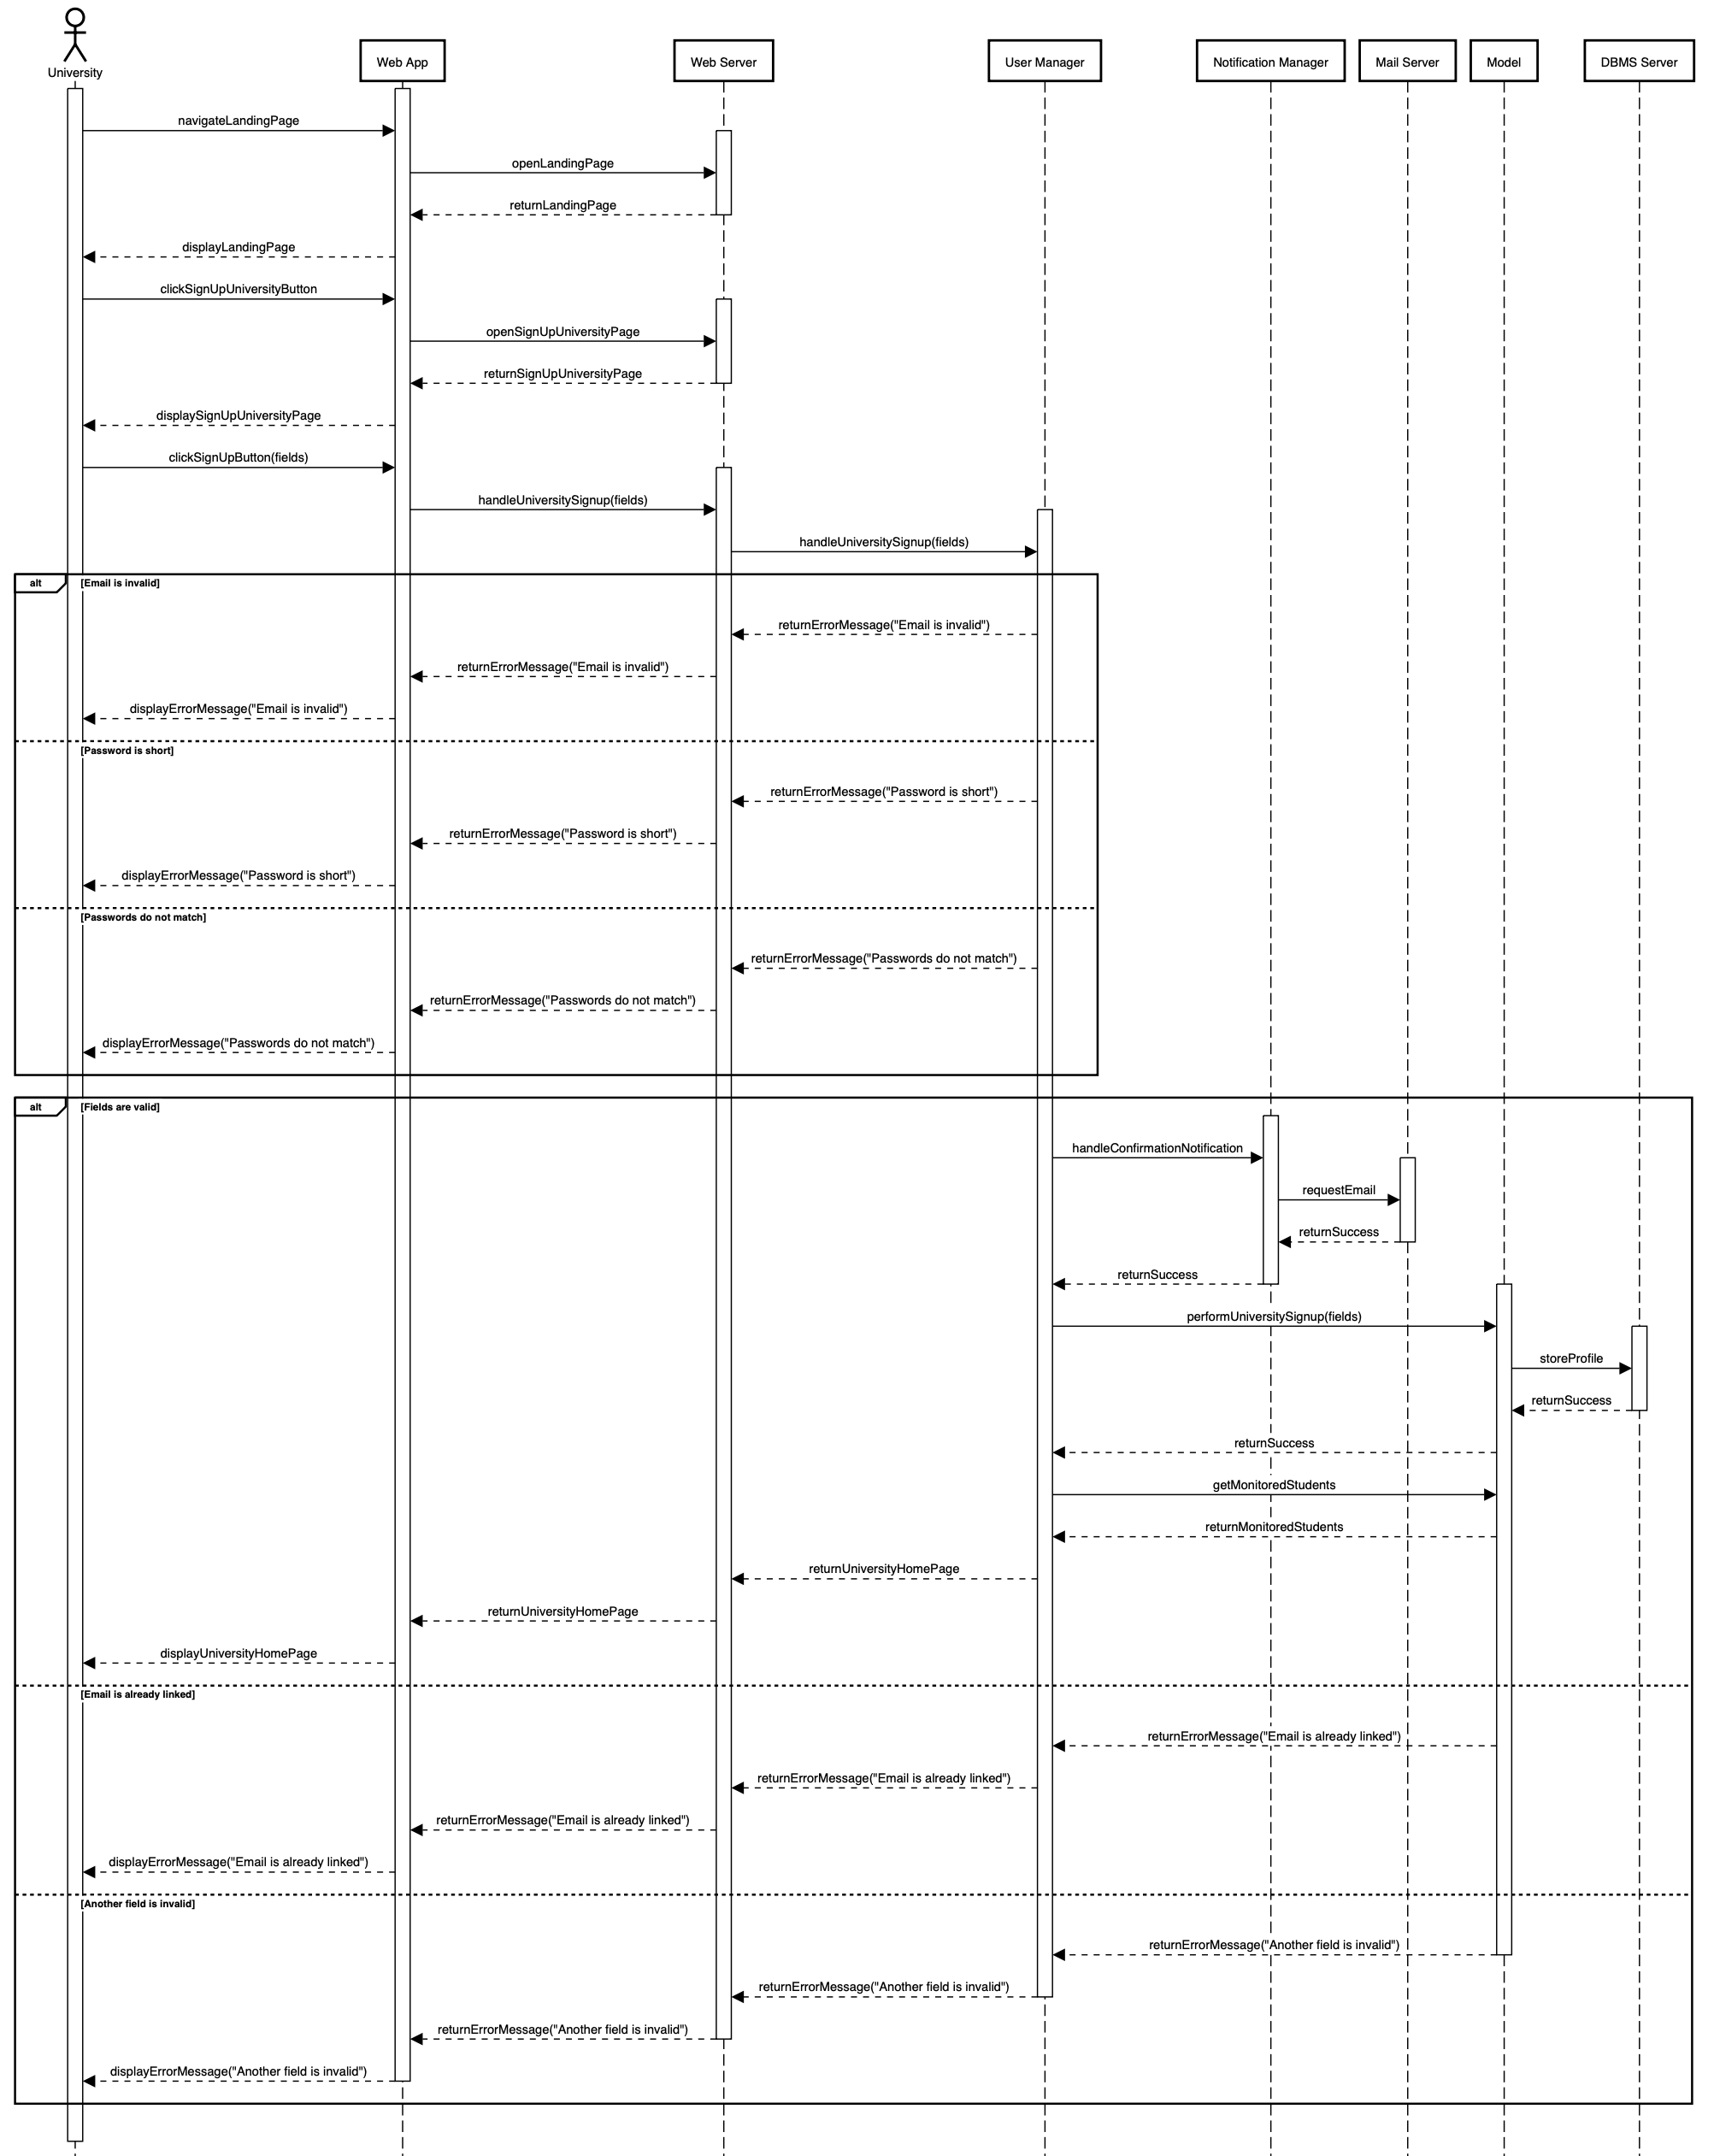
\includegraphics[width=14cm]{images/sequence-diagrams/university-signs-up.png}
    \caption{University signs up sequence diagram}
\end{figure}

\clearpage
\subsubsection{University Logs In}
The university is signed up. 

\begin{figure}[h]
    \centering
    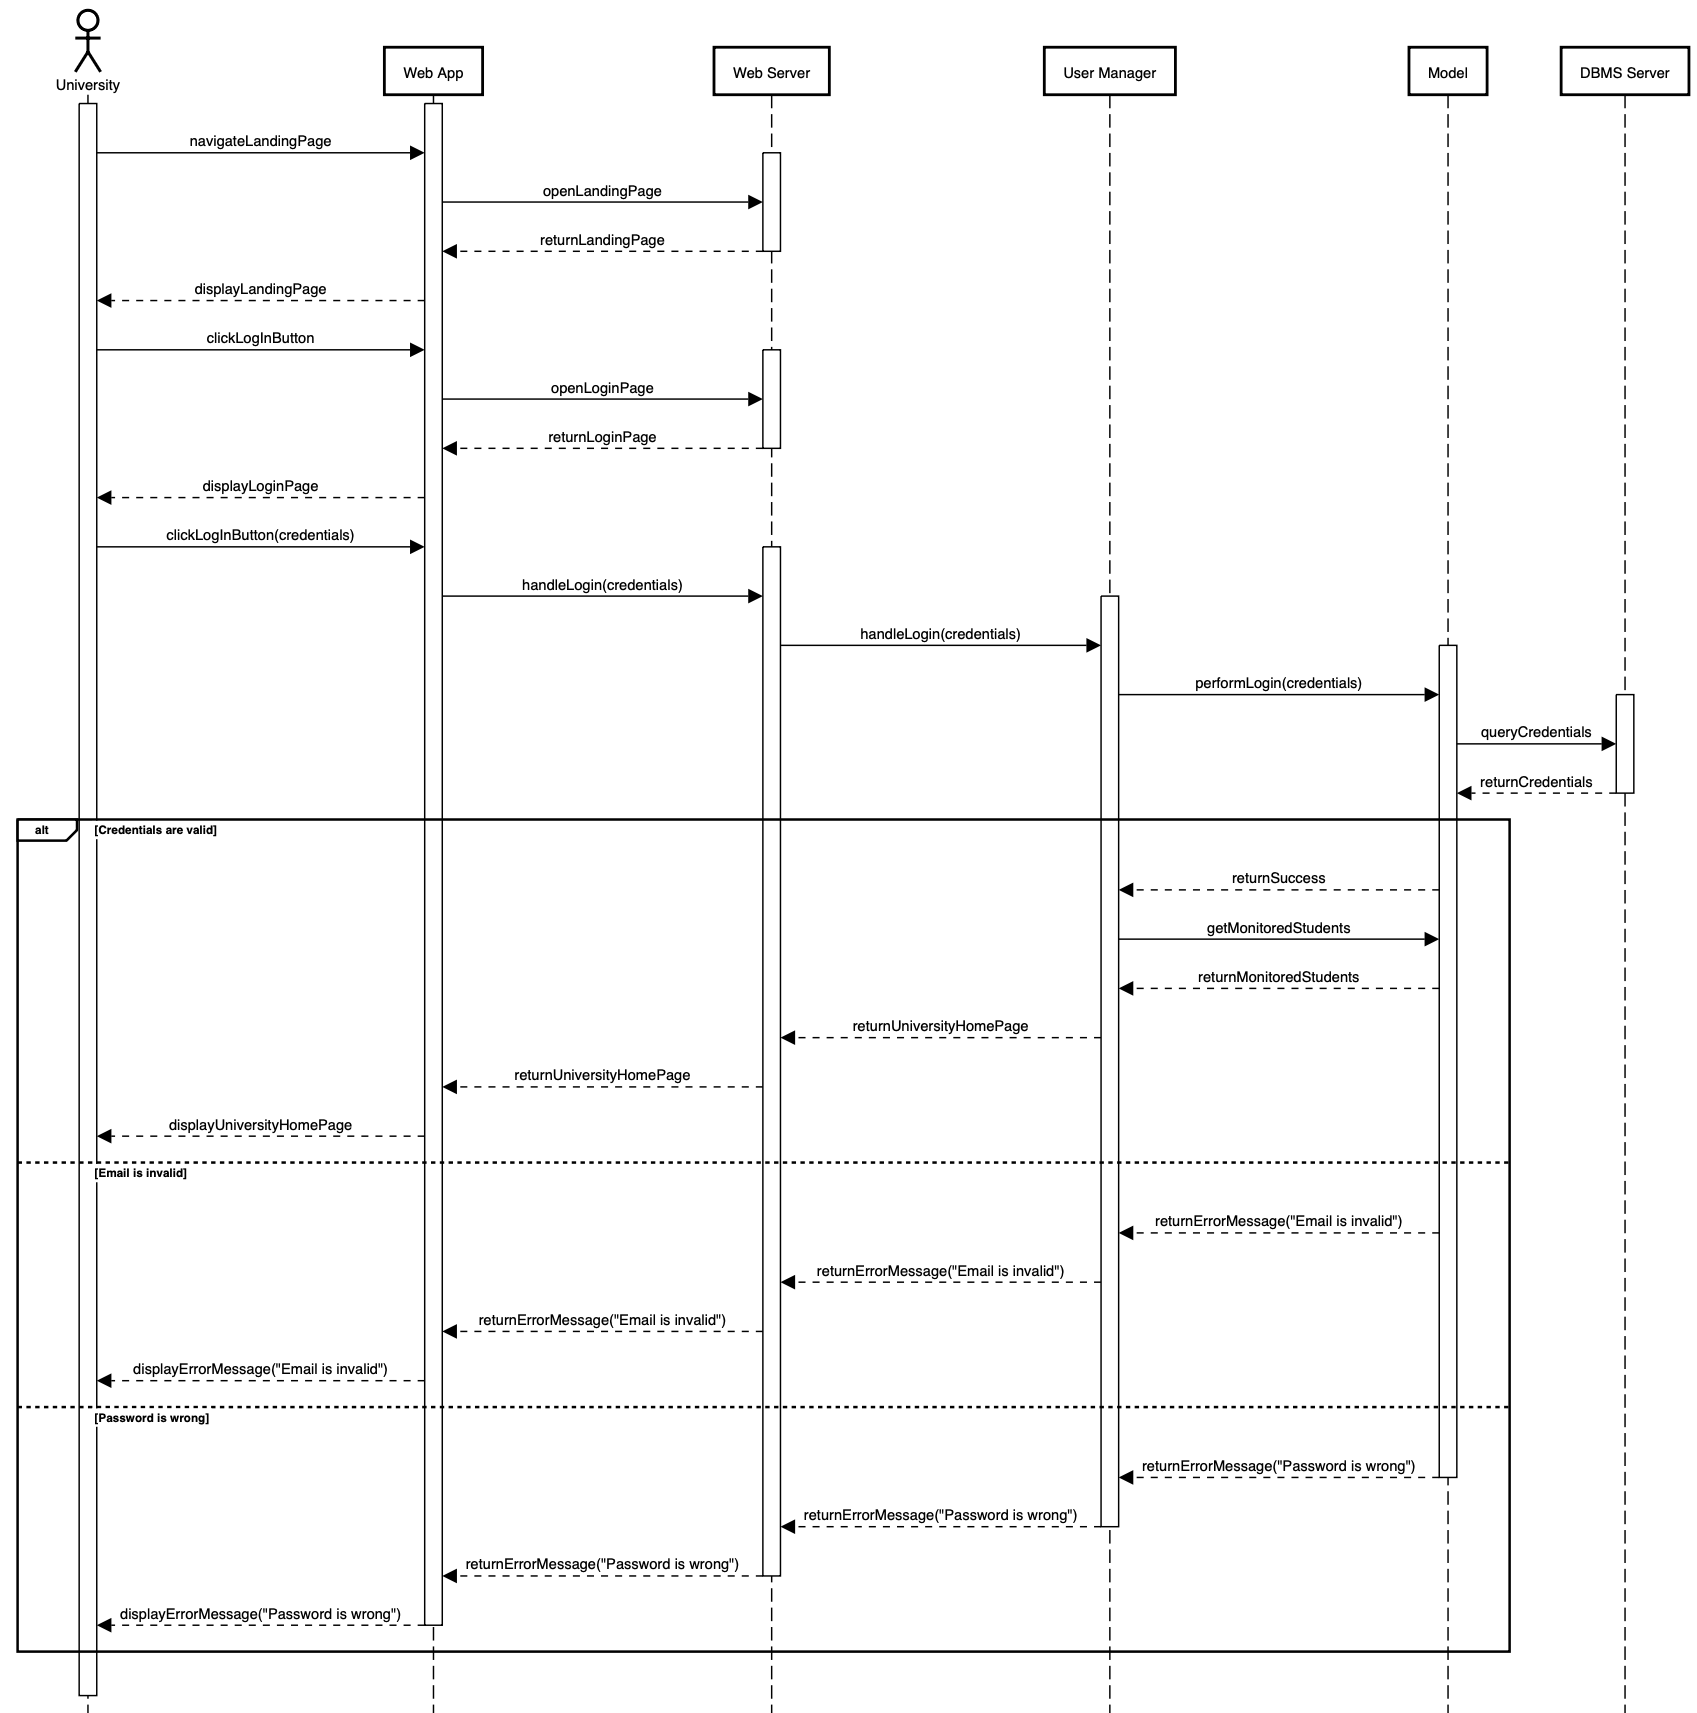
\includegraphics[width=16cm]{images/sequence-diagrams/university-logs-in.png}
    \caption{University logs in sequence diagram}
\end{figure}

\clearpage
\subsubsection{University Comments Internship}
The university is logged in and on the home page.

\begin{figure}[h!] 
    \centering
    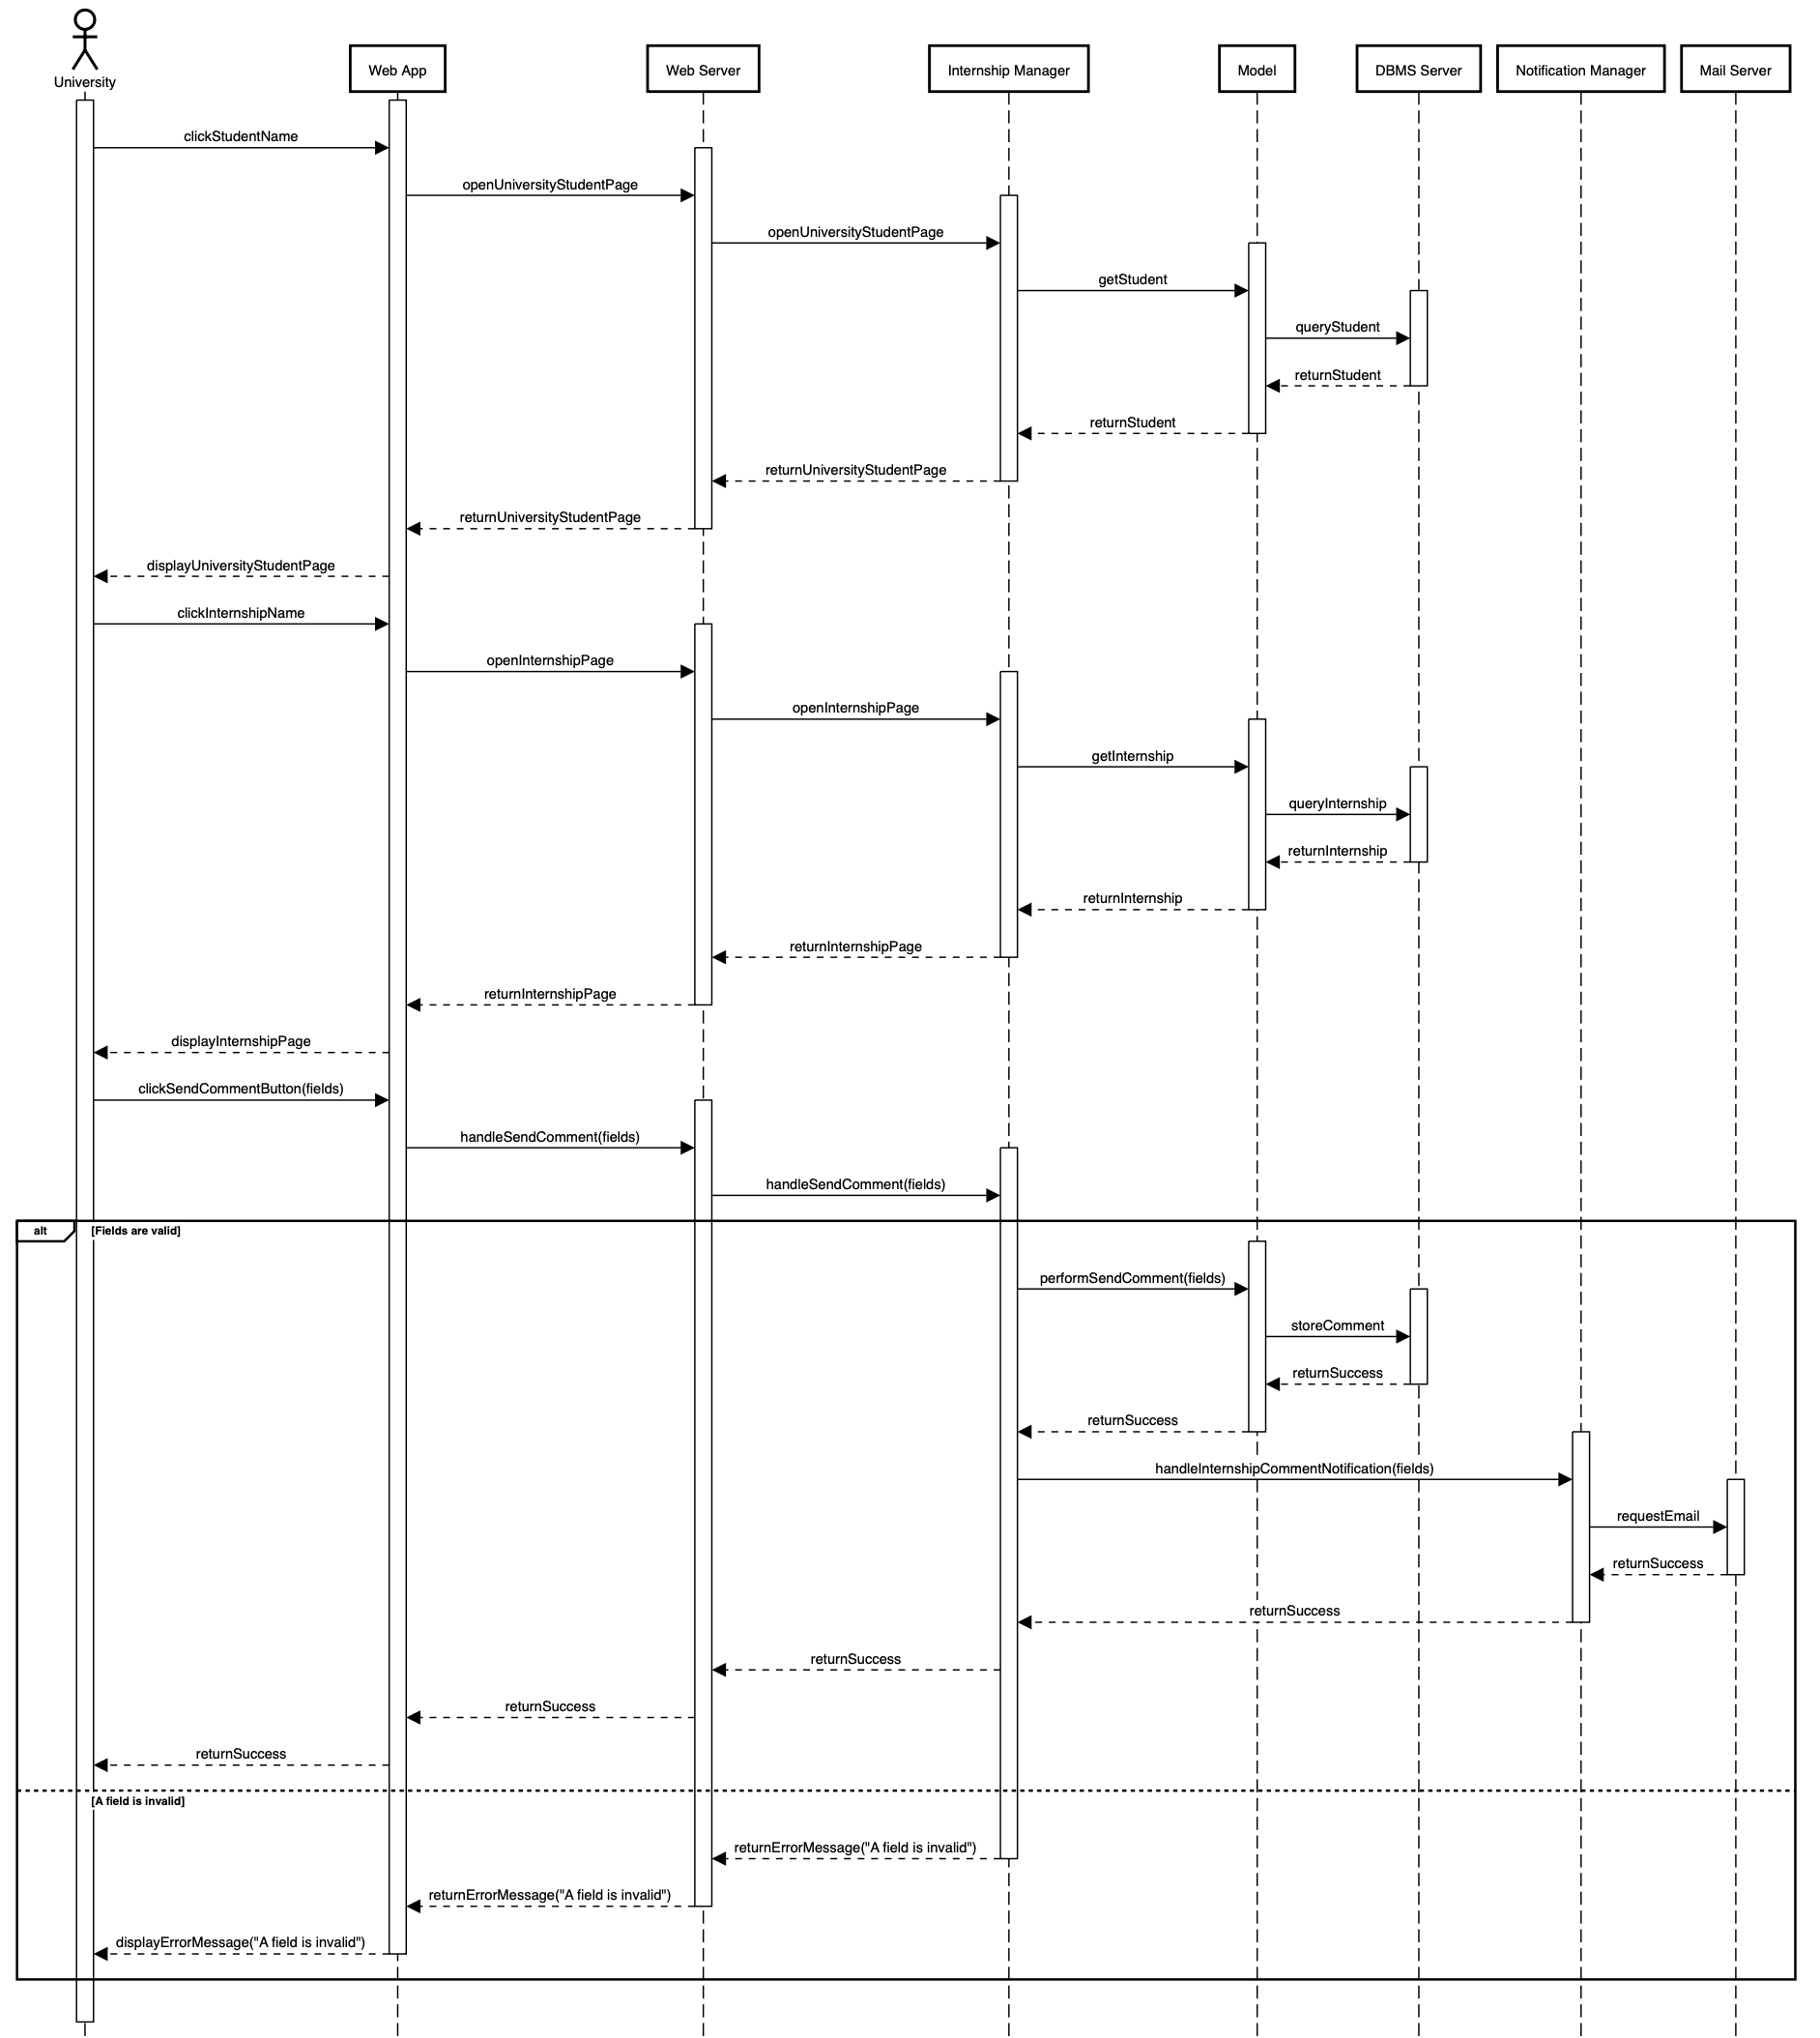
\includegraphics[width=16cm]{images/sequence-diagrams/university-comments-internship.png}
    \caption{University comments internship sequence diagram}
\end{figure}

\clearpage
\section{Component Interfaces}
This section lists the component interfaces that define the methods provided by managers within the system to interact with other components.
Each manager encapsulates a specific set of functionalities and communicates through standardized interfaces to ensure modularity.
For methods requiring database access, there is a corresponding method in the model interface to handle related operations. 
For instance, if the user manager includes the method \texttt{handleUserSignup} to manage user signup, then the model will provide the method \texttt{performUserSignup} to validate and store the data in the database.
This separation ensures a clean architecture by dividing user-facing logic and data-handling responsibilities. 
Note that once a user logs into Students\&Companies, their email is stored in the session.

\renewcommand{\arraystretch}{1.5}
\begin{longtable}{|p{14.5cm}|}
    \hline
    \cellcolor{custompurple}\textbf{User Interface} \\ \hline
    \texttt{handleStudentSignup(String name, String surname, String email, String password, String confirmPassword, boolean keepMeUpdated, String preferences, String cv)} \\ \hline
    \texttt{handleCompanySignup(String name, String email, String field, String password, String confirmPassword, boolean keepMeUpdated)} \\ \hline
    \texttt{handleUniversitySignup(String name, String email, String password, String confirmPassword, boolean keepMeUpdated)} \\ \hline
    \texttt{handleDeleteProfile()} \\ \hline
    \texttt{handleLogin(String email, String password)} \\ \hline
    \texttt{handleLogout()} \\ \hline
    \texttt{handleUpdateStudentProfile(String name, String lastname, String email, String password, String confirmPassword, String preferences, String cv)} \\ \hline
    \texttt{handleUpdateCompanyProfile(String name, String email, String field, String password, String confirmPassword)} \\ \hline
    \texttt{handleUpdateUniversityProfile(String name, String email, String password, String confirmPassword)} \\ \hline
    \texttt{openStudentHomePage()} \\ \hline
    \texttt{openCompanyHomePage()} \\ \hline
    \texttt{openUniversityHomePage()} \\ \hline
    \texttt{openMyProfilePage()} \\ \hline
\caption{User interface}
\end{longtable}

\renewcommand{\arraystretch}{1.5}
\begin{longtable}{|p{14.5cm}|}
    \hline
    \cellcolor{customblue}\textbf{Position Interface} \\ \hline
    \texttt{handlePostPosition(String name, String domain, String project, String tasks, String terms)} \\ \hline
    \texttt{handleDeletePosition(int positionId)} \\ \hline
    \texttt{handleUpdatePosition(int positionId, String domain, String project, String tasks, String terms)} \\ \hline
    \texttt{handleSearchPosition(String keyword)} \\ \hline
    \texttt{openMyPositionsPage()} \\ \hline
    \texttt{openPositionPage(int positionId)} \\ \hline
    \texttt{openStudentPage(String studentEmail)} \\ \hline
    \texttt{openCompanyPage(String companyEmail)} \\ \hline
\caption{Position interface}
\end{longtable}

\renewcommand{\arraystretch}{1.5}
\begin{longtable}{|p{14.5cm}|}
    \hline
    \cellcolor{customgreen}\textbf{Recommendation Interface} \\ \hline
    \texttt{handleAcceptStudentRecommendation(int recommendationId, boolean accepted)} \\ \hline
    \texttt{handleAcceptCompanyRecommendation(int recommendationId, boolean accepted)} \\ \hline
    \texttt{handleFillOutFeedbackForm(List<String> fields)} \\ \hline
\caption{Recommendation interface}
\end{longtable}

\renewcommand{\arraystretch}{1.5}
\begin{longtable}{|p{14.5cm}|}
    \hline
    \cellcolor{customyellow}\textbf{Selection Interface} \\ \hline
    \texttt{handleApplication(int positionId)} \\ \hline
    \texttt{handleWithdrawApplication(int applicationId)} \\ \hline
    \texttt{handleUpdateSelectionStatus(int selectionId, String status)} \\ \hline
    \texttt{handleScheduleInterview(int selectionId, Date date, String mode)} \\ \hline
    \texttt{handleAcceptInterview(int interviewId, boolean accepted)} \\ \hline
    \texttt{handleAddQuestionnaire(int selectionId, List<String> fields)} \\ \hline
    \texttt{handleFillOutQuestionnaire(int questionnaireId, List<String> fields)} \\ \hline
    \texttt{openMyApplicationsPage()} \\ \hline
    \texttt{openApplicationPage(int appplicationId)} \\ \hline
\caption{Selection interface}
\end{longtable}

\renewcommand{\arraystretch}{1.5}
\begin{longtable}{|p{14.5cm}|}
    \hline
    \cellcolor{customorange}\textbf{Internship Interface} \\ \hline
    \texttt{handleUpdateInternshipStatus(int internshipId, String status)} \\ \hline
    \texttt{handleSendComment(int internshipId, String comment)} \\ \hline
    \texttt{openMyInternshipsPage()} \\ \hline
    \texttt{openInternshipPage(int internshipId)} \\ \hline
\caption{Internship interface}
\end{longtable}

\renewcommand{\arraystretch}{1.5}
\begin{longtable}{|p{14.5cm}|}
    \hline
    \cellcolor{customred}\textbf{Notification Interface} \\ \hline
    \texttt{handleConfirmationNotification(String email)} \\ \hline
    \texttt{handleStudentApplicationNotification(String studentEmail, int applicationId)} \\ \hline
    \texttt{handleCompanyApplicationNotification(String companyEmail, int applicationId)} \\ \hline
    \texttt{handleRecommendationNotification(String studentEmail, String companyEmail, int recommendationId)} \\ \hline
    \texttt{handleMatchNotification(String studentEmail, String companyEmail, int recommendationId)} \\ \hline
    \texttt{handleSelectionStatusNotification(String studentEmail, String companyEmail, int selectionId)} \\ \hline
    \texttt{handleScheduledInterviewNotification(String studentEmail, int interviewId)} \\ \hline
    \texttt{handleAcceptedInterviewNotification(String companyEmail, int interviewId, boolean accepted)} \\ \hline
    \texttt{handleAddedQuestionnaireNotification(String studentEmail, int questionnaireId)} \\ \hline
    \texttt{handleFilledOutQuestionnaireNotification(String companyEmail, int questionnaireId)} \\ \hline
    \texttt{handleInternshipStatusNotification(String studentEmail, String companyEmail, String universityEmail, int internshipId, String status)} \\ \hline
    \texttt{handleInternshipCommentNotification(String studentEmail, String companyEmail, String universityEmail, int internshipId, String authorEmail, String comment)} \\ \hline
\caption{Notification interface}
\end{longtable}

\renewcommand{\arraystretch}{1.5}
\begin{longtable}{|p{14.5cm}|}
    \hline
    \cellcolor{customgrey}\textbf{Model Interface} \\ \hline
    \texttt{performStudentSignup(String name, String surname, String email, String password, boolean keepMeUpdated, String preferences, String cv)} \\ \hline
    \texttt{performCompanySignup(String name, String email, String field, String password, boolean keepMeUpdated)} \\ \hline
    \texttt{performUniversitySignup(String name, String email, String password, boolean keepMeUpdated)} \\ \hline
    \texttt{performDeleteProfile(String email)} \\ \hline
    \texttt{performLogin(String email, String password)} \\ \hline
    \texttt{performUpdateStudentProfile(String name, String lastname, String email, String password, String preference, String cv)} \\ \hline
    \texttt{performUpdateCompanyProfile(String name, String email, String field, String password)} \\ \hline
    \texttt{performUpdateUniversityProfile(String name, String email, String password)} \\ \hline
    \texttt{getRecommendedPositions(String studentEmail)} \\ \hline
    \texttt{getRecommendedStudents(String companyEmail)} \\ \hline
    \texttt{getMonitoredStudents(String universityEmail)} \\ \hline
    \texttt{getProfile(String email)} \\ \hline

    \texttt{performPostPosition(String companyEmail, String name, String domain, String project, String tasks, String terms)} \\ \hline
    \texttt{performDeletePosition(int positionId)} \\ \hline
    \texttt{performUpdatePosition(int positionId, String name, String domain, String project, String tasks, String terms)} \\ \hline
    \texttt{performSearchPosition(String keyword)} \\ \hline
    \texttt{getPositions(String companyEmail)} \\ \hline
    \texttt{getPosition(positionId)} \\ \hline

    \texttt{performAcceptStudentRecommendation(int recommendationId, boolean accepted)} \\ \hline
    \texttt{performAcceptCompanyRecommendation(int recommendationId, boolean accepted)} \\ \hline
    \texttt{performFillOutFeedbackForm(String email, List<String> fields)} \\ \hline
    
    \texttt{performApplication(String studentEmail, int positionId)} \\ \hline
    \texttt{performWithdrawApplication(int applicationId)} \\ \hline
    \texttt{performUpdateSelectionStatus(String email, int selectionId, String status)} \\ \hline
    \texttt{performScheduleInterview(int selectionId, String description, Date date, String mode)} \\ \hline
    \texttt{performAcceptInterview(int interviewId, boolean accepted)} \\ \hline
    \texttt{performAddQuestionnaire(int selectionId, List<String> fields)} \\ \hline
    \texttt{performFillOutQuestionnaire(int questionnaireId, List<String> fields)} \\ \hline
    \texttt{getApplications(String studentEmail)} \\ \hline
    \texttt{getApplication(int applicationId)} \\ \hline
    
    \texttt{performUpdateInternshipStatus(String email, int internshipId, String status)} \\ \hline
    \texttt{performSendComment(String email, int internshipId, String comment)} \\ \hline
    \texttt{getInternships(String email)} \\ \hline
    \texttt{getInternship(int internshipId)} \\ \hline
\caption{Model interface}
\end{longtable}

\section{Architectural Styles and Patterns}
This section examines the architectural styles adopted in Students\&Companies, explaining their general principles and how they guide implementation decisions.
Understanding these foundational patterns is crucial for developers working on the system, as they influence everything from component interaction to code organization.

\subsubsection{Client-Server Architecture}
The system's foundation rests on a client-server architecture, which separates components into service requesters, called clients, and service providers, called servers.
This separation enables the user interface to evolve independently from data processing and storage, while centralizing resource management on the server.
Developers can thus focus on their domain, either crafting responsive user experiences or implementing robust business logic.

Modern applications refine this pattern through tiers, which are logical groupings of related functionality.
A three-tier architecture divides the application into three distinct layers: a presentation tier that handles the user interface, an application tier that processes business logic and a data tier that manages storage.
This separation gives developers clear boundaries for their work and lets teams works independently, reducing development bottlenecks and simplifying maintenance.

\subsubsection{REST Architecture}
REST (Representational State Transfer) guides how these tiers communicate over the web.
Originally conceived for document transfer, REST has evolved into a comprehensive style for data exchange.
Its core principle of statelessness means that servers maintain no information about past requests.
Instead, each client request must contain all necessary context.
This architectural choice significantly impacts development: backend developers do not need to manage session states, system administrators benefit from straightforward load balancing since any server can handle any request and cache developers can optimize performance by focusing on request parameters rather than server state.

\subsubsection{MVC Pattern}
The Model-View-Controller (MVC) pattern organizes software into three interconnected components, each with distinct responsibilities.
The model represents the core data structure, encapsulating the database, while the view handles user interaction and presentation.
Controllers act as intermediaries, processing user requests to run business logic and coordinate workflows.
This separation of concerns enhances scalability, modularity and maintainability, allowing developers to focus on specific aspects of the system without impacting others, ultimately fostering efficient collaboration among teams.

\section{Other Design Decisions}
While architectural styles and patterns provide the system's foundation, many other critical design decisions shape its implementation.
This section outlines these choices, focusing on practical aspects that developers must consider when implementing the system.

\subsubsection{Deployment Approach}
The deployment strategy embraces horizontal scaling, running multiple application server instances rather than scaling up individual servers.
This approach requires developers to write stateless code that works across instances, but provides significant benefits: the system continues functioning even if some instances fail, resource allocation becomes more flexible as administrators can add or remove instances based on demand and load balancing becomes straightforward since any instance can handle any request.

\subsubsection{Security Implementation}
Security permeates every aspect of the design through multiple complementary layers: all client-server communication uses HTTPS encryption to protect data in transit, sensitive information receives additional encryption in the database and session management relies on time-limited tokens rather than storing session data on the server.

\subsubsection{Data Management}
Data management emphasizes both integrity and performance: the database implements transaction management to maintain consistency even during concurrent operations, constraint enforcement catches validity issues early and performance optimization through strategic indexing and caching improves response times.
